%----------------------------------------------------------------------------------------
%	PACKAGES AND OTHER DOCUMENT CONFIGURATIONS
%----------------------------------------------------------------------------------------

\documentclass[
11pt, % The default document font size, options: 10pt, 11pt, 12pt
%oneside, % Two side (alternating margins) for binding by default, uncomment to switch to one side
english, % ngerman for German
singlespacing, % Single line spacing, alternatives: onehalfspacing or doublespacing
%draft, % Uncomment to enable draft mode (no pictures, no links, overfull hboxes indicated)
%nolistspacing, % If the document is onehalfspacing or doublespacing, uncomment this to set spacing in lists to single
%liststotoc, % Uncomment to add the list of figures/tables/etc to the table of contents
%toctotoc, % Uncomment to add the main table of contents to the table of contents
%parskip, % Uncomment to add space between paragraphs
%nohyperref, % Uncomment to not load the hyperref package
headsepline, % Uncomment to get a line under the header
%chapterinoneline, % Uncomment to place the chapter title next to the number on one line
%consistentlayout, % Uncomment to change the layout of the declaration, abstract and acknowledgements pages to match the default layout
]{MastersDoctoralThesis} % The class file specifying the document structure

\usepackage[utf8]{inputenc} % Required for inputting international characters
\usepackage[T1]{fontenc} % Output font encoding for international characters
%\usepackage{mathpazo} % Use the Palatino font by default
\usepackage[libertine,cmintegrals,cmbraces,vvarbb]{newtxmath}
\usepackage[scaled=0.95]{inconsolata}
%\usepackage[backend=bibtex,style=authoryear,natbib=true]{biblatex} % Use the bibtex backend with the authoryear citation style (which resembles APA)
\usepackage[backend=bibtex]{biblatex} 
\addbibresource{cryptobib/abbrev3.bib} % The filename of the bibliography
\addbibresource{cryptobib/crypto.bib}
\addbibresource{custombib/journal_ref.bib}

\usepackage[autostyle=true]{csquotes} % Required to generate language-dependent quotes in the bibliography
\usepackage{amsmath}
\usepackage{graphicx, layout, url}
\usepackage{latexsym}
\usepackage{amssymb} 
\usepackage{hhline}
\usepackage{enumerate}
%\usepackage{Amsfonts}
\usepackage{color}
\usepackage[abs]{overpic}
\usepackage{multirow}
\usepackage{eepic}
%\usepackage{algorithm}
%\usepackage{algorithmic}
\usepackage{ascmac,styleFiles/eclbkbox}
\usepackage{amscd}
\usepackage{geometry}
\usepackage[final]{styleFiles/nogamacro}
\usepackage[final]{styleFiles/nogaref}
\usepackage[ruled,vlined]{algorithm2e}
\usepackage[makeroom]{cancel}
\usepackage{romannum}
\usepackage{tabularx, booktabs}
\usepackage{styleFiles/manyeqns}
%\usepackage{MinionPro}
%----------------------------------------------------------------------------------------
%	MARGIN SETTINGS
%----------------------------------------------------------------------------------------

\geometry{
	paper=a4paper, % Change to letterpaper for US letter
	inner=2.5cm, % Inner margin
	outer=3.8cm, % Outer margin
	bindingoffset=.5cm, % Binding offset
	top=1.5cm, % Top margin
	bottom=1.5cm, % Bottom margin
	%showframe, % Uncomment to show how the type block is set on the page
}

%----------------------------------------------------------------------------------------
%	THESIS INFORMATION
%----------------------------------------------------------------------------------------

\thesistitle{Proposals on Efficient Software Implementation of Pairing-Based Cryptographic Primitives} % Your thesis title, this is used in the title and abstract, print it elsewhere with \ttitle
\supervisor{Dr. Yasuyuki \textsc{Nogami}} % Your supervisor's name, this is used in the title page, print it elsewhere with \supname
\examiner{} % Your examiner's name, this is not currently used anywhere in the template, print it elsewhere with \examname
\degree{Doctor of Philosophy} % Your degree name, this is used in the title page and abstract, print it elsewhere with \degreename
\author{Md. Al-Amin \textsc{Khandaker}} % Your name, this is used in the title page and abstract, print it elsewhere with \authorname
\addresses{} % Your address, this is not currently used anywhere in the template, print it elsewhere with \addressname

\subject{Biological Sciences} % Your subject area, this is not currently used anywhere in the template, print it elsewhere with \subjectname
\keywords{} % Keywords for your thesis, this is not currently used anywhere in the template, print it elsewhere with \keywordnames
\university{\href{http://www.okayama-u.ac.jp}{Okayama University}} % Your university's name and URL, this is used in the title page and abstract, print it elsewhere with \univname
\department{\href{https://www.gnst.okayama-u.ac.jp}{Graduate School of Natural Science and Technology}} % Your department's name and URL, this is used in the title page and abstract, print it elsewhere with \deptname
\group{\href{http://isec.ec.okayama-u.ac.jp}{Information Security Lab.}} % Your research group's name and URL, this is used in the title page, print it elsewhere with \groupname
\faculty{\href{http://faculty.university.com}{Faculty of Engineering}} % Your faculty's name and URL, this is used in the title page and abstract, print it elsewhere with \facname

\AtBeginDocument{
\hypersetup{pdftitle=\ttitle} % Set the PDF's title to your title
\hypersetup{pdfauthor=\authorname} % Set the PDF's author to your name
\hypersetup{pdfkeywords=\keywordnames} % Set the PDF's keywords to your keywords
}

\newtheorem{definition}{Definition}
\newtheorem{remark}{Remark}
\newtheorem{property}{Property}
\newtheorem{theorem}{Theorem}
\newtheorem{example}{Example}[chapter]
\newcommand\proof[1]{{\bf \sya{Proof} (#1) : }}
\newcommand{\qed}{\hfill\rule{1.8mm}{1.8mm}}
\newcommand\algref[1]{{\bf Algorithm #1}}

\newcommand{\es}{\ \ \ \ \ }
\newcommand{\esa}{&\es = &\es}
\def\sp{\vspace{3pt}}
\newcommand\Inf{\mathcal{O}}
\newcommand{\FQ}{\mathbb{F}_p}
\newcommand{\EFQ}{E(\mathbb{F}_q)}
\newcommand{\EFP}{E(\mathbb{F}_p)}
\newcommand{\SEFQ}{\#E(\mathbb{F}_q)}
\newcommand{\SEFP}{\#E(\mathbb{F}_p)}
\newcommand{\FQK}{\mathbb{F}_{p^k}}
\newcommand{\FQTH}{\mathbb{F}_{p^3}}
\newcommand{\FQTHTW}{\mathbb{F}_{(p^3)^2}}
\newcommand{\FQTHTWTH}{\mathbb{F}_{((p^3)^2)^3}}
\newcommand{\FQSX}{\mathbb{F}_{p^6}}
\newcommand{\FQTV}{\mathbb{F}_{p^{12}}}
\newcommand{\FQEN}{\mathbb{F}_{p^{18}}}
\newcommand{\GT}{\mathbb{G}_T}
\newcolumntype{Y}{>{\centering\arraybackslash}X}

\newcommand\Fpiii{\ensuremath{\mathbb{F}_{p^{3}}}}
\newcommand\Fpvi{\ensuremath{\mathbb{F}_{p^{6}}}}
\newcommand\Fpxviii{\ensuremath{\mathbb{F}_{p^{18}}}}
\newcommand{\G}[1]{\mathbb{G}_{#1}}
\newcommand{\Fpk}{\mathbb{F}_{p^k}}
%\newcommand{\EFp}[1]{E(\mathbb{F}_{p^{#1}})}
%\newcommand{\FQ}{\mathbb{F}_p}
%\newcommand{\EFQ}{E(\mathbb{F}_p)}
%\newcommand{\EFP}{E(\mathbb{F}_p)}
%\newcommand{\SEFQ}{\#E(\mathbb{F}_p)}
%\newcommand{\SEFP}{\#E(\mathbb{F}_p)}
%\newcommand{\FQK}{\mathbb{F}_{p^k}}
%\newcommand{\FQTH}{\mathbb{F}_{p^3}}
%\newcommand{\FQTHTW}{\mathbb{F}_{(p^3)^2}}
%\newcommand{\FQTHTWTH}{\mathbb{F}_{((p^3)^2)^3}}
%\newcommand{\FQSX}{\mathbb{F}_{p^6}}
%\newcommand{\FQTV}{\mathbb{F}_{p^{12}}}
%\newcommand{\FQEN}{\mathbb{F}_{p^{18}}}
%\newcommand{\GT}{\mathbb{G}_T}

\makeatletter
\newcommand{\extraPartText}[1]{\def\@extraPartText{#1}}
\pretocmd{\@endpart}{\vspace{8ex}\begingroup\centering\@extraPartText\par\endgroup\let\@extraPartText\relax}{}{}
\makeatother

\begin{document}

\frontmatter % Use roman page numbering style (i, ii, iii, iv...) for the pre-content pages

\pagestyle{plain} % Default to the plain heading style until the thesis style is called for the body content

%----------------------------------------------------------------------------------------
%	TITLE PAGE
%----------------------------------------------------------------------------------------

\begin{titlepage}
\begin{center}

\vspace*{.06\textheight}
% {\scshape\LARGE \univname\par}\vspace{1.5cm} % University name
\textsc{\Large Doctoral Thesis}\\[0.5cm] % Thesis type

\HRule \\[0.4cm] % Horizontal line
{\huge \bfseries \ttitle\par}\vspace{0.4cm} % Thesis title
\HRule \\[1.5cm] % Horizontal line
 
\begin{minipage}[t]{0.4\textwidth}
\begin{flushleft} \large
\emph{Author:}\\
{\authorname} % Author name - remove the \href bracket to remove the link
\end{flushleft}
\end{minipage}
\begin{minipage}[t]{0.4\textwidth}
\begin{flushright} \large
\emph{Supervisor:} \\
\href{http://isec.ec.okayama-u.ac.jp/nogami}{\supname} % Supervisor name - remove the \href bracket to remove the link  
\end{flushright}
\end{minipage}\\[3cm]
 
\vfill

\large \textit{A thesis submitted in fulfillment of the requirements\\ for the degree of \degreename}\\[0.3cm] % University requirement text
\textit{in the}\\[0.4cm]
\groupname\\\deptname\\[2cm] % Research group name and department name
{\scshape\LARGE \univname\par}\vspace{1.5cm} % University name

\includegraphics[scale = 0.1]{okadailogo} \\ % \\ University/department logo - uncomment to place it
\vfill
{\large \today}\\[4cm] % Date
\vfill
\end{center}
\end{titlepage}

%----------------------------------------------------------------------------------------
%	DECLARATION PAGE
%----------------------------------------------------------------------------------------

\begin{declaration}
	
\addchaptertocentry{\authorshipname} % Add the declaration to the table of contents
\noindent This dissertation and the work presented here for doctoral studies were conducted under the supervision of Professor Yasuyuki Nogami.
 I, \authorname, declare that this thesis titled, \enquote{\ttitle} and the work presented in it are my own. I confirm that:

\begin{itemize} 
\item 
%This work was done wholly or mainly while in candidature for a research degree at this University.
The work presented in this thesis is the result of original research carried out by myself, in collaboration with others, while enrolled in the Faculty of Engineering of Okayama University as a candidate for the degree of Doctor of Philosophy.

\item This work has not been submitted for a degree or any other qualification at this University or any other institution. 
 
\item  Some of the work presented in this thesis was previously published is listed in ``Research Activity'' \ref{research_activity}.

\item The published work of others cited in this thesis is clearly attributed.
%\item Where I have quoted from the work of others, the source is always given. With the exception of such quotations, this thesis is entirely my own work.
\item I have acknowledged all main sources of help to pursue this work.
%\item Where the thesis is based on work done by myself jointly with others, I have made clear exactly what was done by others and what I have contributed myself.
 \item In all works all my coauthors contributed equally. 
 \item The experiments and results presented in this thesis and in the articles where I am the first author were conducted by myself.\\
\end{itemize}
 
\noindent Signed:\\ 
\rule[0.5em]{25em}{0.5pt}
 % This prints a line for the signature\authorname
 
\noindent Date:\\
\rule[0.5em]{25em}{0.5pt} % This prints a line to write the date
\end{declaration}

\cleardoublepage

%----------------------------------------------------------------------------------------
%	QUOTATION PAGE
%----------------------------------------------------------------------------------------

\vspace*{0.2\textheight}

\noindent\enquote{\itshape If we knew what it was we were doing, it would not be called research, would it?
}\bigbreak

\hfill Albert Einstein

%----------------------------------------------------------------------------------------
%	ABSTRACT PAGE
%----------------------------------------------------------------------------------------

\begin{abstract}
\addchaptertocentry{\abstractname} % Add the abstract to the table of contents
The Thesis Abstract is written here (and usually kept to just this page). The page is kept centered vertically so can expand into the blank space above the title too\ldots
\end{abstract}

%----------------------------------------------------------------------------------------
%	ACKNOWLEDGEMENTS
%----------------------------------------------------------------------------------------

\begin{acknowledgements}
\addchaptertocentry{\acknowledgementname} % Add the acknowledgements to the table of contents
The last 3 and a half year is one of the best time of my life I will cherish forever. 
I'm immensely blessed throughout this period for which I have many people to thank.
I'm grateful to many people who have directly and indirectly helped me finish this work.

\vspace{5pt}
This work would not be possible without the unceasing supervision, innumerable counseling and unrelenting persuasion of my Ph.D. advisor Professor Yasuyuki Nogami.
I am indebted to \textit{Nogami Sensei} for having me in his lab \textit{(Information Security Lab.)} as a doctoral student and mentoring me on this work.
He taught me how to analyze complex problems from different perspectives and express the ideas from pen and papers to a fully publishable article.
I enjoyed his insightful comments on the research topics during our discussions.
Sometimes his in-depth queries bewildered me and influenced my ideas in this thesis.
He guided me in different ways to approach a problem and the need to be persistent to accomplish my goal.
His presence and off-work discussion makes the lab more than a workplace. 

\vspace{5pt}
I’m also very grateful for to my doctoral course co-supervisors Professor Nobuo Funabiki (\textit{Distributed Systems Design Lab.}) and Professor Satoshi Denno (\textit{Multimedia Radio Systems Lab}) for having their time to read my thesis draft.
Their insightful comments and helpful advice helped to shape the thesis into this state.
I must recall my experience of talking the “Theory of Distributed Algorithm” course taught by Professor Nobuo Funabiki.
His strong passion for algorithmic problem solving during the lectures were not only inspiring but also contagious. 

\vspace{5pt}
I reminisce my encounters with Professor Satoshi Denno during my days at \textit{Secure Wireless System lab}.
He provided me the  deep-seated idea of the research works and japan life.
His questions and suggestions for the time of half yearly progress meetings was very intuitive. 

\vspace{5pt}
I am very grateful to Associate Professor \mbox{Nobumoto Yamane} of \textit{Information Transmission Lab.} who provided  important comments at progress meetings.

\vspace{5pt}
I would like to express my gratitude to Senior Assistant Professor Takuya Kusaka of \textit{(Information Security Lab.)} for our in depth discussion of  scientific topics.
His strong work ethics and passion for research helped us to publish some of the remarkable collaborative works. 
His was always there to help  while any difficulty arose for attending a conference to publishing a paper.  

\vspace{5pt}
I express my gratitude to Senior Assistant Professor Hiroto Kagotani of \textit{Information System Design Lab} for employing me as a research assistant for a quarter. 
Since \textit{Information System Design Lab} and \textit{(Information Security Lab.)} share space, we had encountered more often and share off research discussions.
His comments during the progress report was enlightening.

\vspace{5pt}
I am also grateful to Assistant Professor Kengo Iokibe (\textit{Optical and Electromagnetic Waves Laboratory}) for the collaborative work we had on side-channel analysis of raspberry pi.

\vspace{5pt}
I would like to express my deep gratitude of Professor Sylvain Duquesne of  Univ  Rennes, France for having me at IRMAR as a short term researcher and allowing me to present my work in front of some brightest audiences.
Professor Duquesne's in-depth reviews on my works was not only helpful towards to final acceptability but also intriguing.   
My sincere gratitude post-doctoral fellow Dr. Loubna Ghammam at Normandie University, France for her persistent guidance.
Our collaboration with  Professor Duquesne and Dr. Loubna helps me to work on diverse area of mathematical aspects of cryptography.

\vspace{5pt}
I am also thankful to Professor Howon Kim of Pusan National University, South Korea and his Ph.D. student Taehwan Park for  a great research collaboration on IoT security.
My gratitude to one of the great IoT security expert Professor Hwajeong Seo of Hansung University, South Korea for being a co-author in my first major conference paper.

\vspace{5pt}
Thanks to MEXT, Japan  for the scholarship which fulfilled my dream to pursue the  doctoral study in Japan possible.
I sincere acknowledge all the funds that afforded me to join several international conferences and conduct research activities.
 
 \vspace{5pt}
I am also grateful to all  administrative officer of Faculty of Engineering who directly or indirectly made an impact in my doctoral course studies. My especial thanks to Ms. Yumiko Kurooka for kind supports in administrative documents.

\vspace{5pt}
Special thanks also to my seniors, juniors, and friends in the  laboratory for creating a great work atmosphere and  their generous support.  
Thanks to pairing team members of my lab who are one of brightest minds I've worked with.

\vspace{5pt}
I can not thank enough to my wife Mashrufee Alam (Shama) for her sacrifices and generous supports to my bread and butter. 
I would like to take the opportunity to appreciate my parents Ms. Nasima Akter and Mr. Md. Ali-Azzam Khandaker for their understanding, and encouragements.

\vspace{5pt}
So far so general we all are standing on shoulders giants for our works. 
My profound gratitude to all great cryptographer, cryptographic engineers and researchers whose works keep inspiring students like me.
I'm indebted to all my research collaborator, co-authors and reviewers for making my doctoral voyage engaging.


%The acknowledgments and the people to thank go here, don't forget to include your project advisor\ldots
\end{acknowledgements}

%----------------------------------------------------------------------------------------
%	LIST OF CONTENTS/FIGURES/TABLES PAGES
%----------------------------------------------------------------------------------------

\tableofcontents % Prints the main table of contents

\listoffigures % Prints the list of figures

\listoftables % Prints the list of tables

%----------------------------------------------------------------------------------------
%	ABBREVIATIONS
%----------------------------------------------------------------------------------------

\begin{abbreviations}{ll} % Include a list of abbreviations (a table of two columns)

\textbf{LAH} & \textbf{L}ist \textbf{A}bbreviations \textbf{H}ere\\
\textbf{WSF} & \textbf{W}hat (it) \textbf{S}tands \textbf{F}or\\

\end{abbreviations}

%----------------------------------------------------------------------------------------
%	PHYSICAL CONSTANTS/OTHER DEFINITIONS
%----------------------------------------------------------------------------------------

%\begin{constants}{lr@{${}={}$}l} % The list of physical constants is a three column table
% The \SI{}{} command is provided by the siunitx package, see its documentation for instructions on how to use it
%Speed of Light & $c_{0}$ & \SI{2.99792458e8}{\meter\per\second} (exact)\\
%Constant Name & $Symbol$ & $Constant Value$ with units\\
%\end{constants}

%----------------------------------------------------------------------------------------
%	SYMBOLS
%----------------------------------------------------------------------------------------

\begin{symbols}{lll} % Include a list of Symbols (a three column table)
Notation & Description & \\
\addlinespace
$p$ &  $p > 3$  is an odd prime integer in this thesis. &\\
$x \bmod p$ & Modulo operation. the least nonnegative residue of $x$ modulo $p$. &\\
\Fp & Prime field. The field of integers mod $p$. \\
\mFp &  The multiplicative group of the field \Fp. In other words, $\mFp=\{x| \ x\in \Fp\ {\rm and}\ x\neq 0\}$. & \\
%$k\in _{R}[1,\ n-1]$ & $1\ls k\ls n-1$ is a randomly selected integer. & \\
$\lfloor \cdot \rfloor$ &  The floor of $\cdot$ is the greatest integer less than or  equal to $\cdot$. & \\
  & For example, $\lfloor 1 \rfloor=1$ and $\lfloor 6.3 \rfloor=6$. & \\
%%$P$ & power & \si{\watt} (\si{\joule\per\second}) \\
%Symbol & Name & Unit \\

%\addlinespace % Gap to separate the Roman symbols from the Greek

%$\omega$ & angular frequency & \si{\radian} \\

\end{symbols}

%----------------------------------------------------------------------------------------
%	DEDICATION
%----------------------------------------------------------------------------------------

\dedicatory{
	Dedicated to two ladies I owe most. 
My mother who brought me to this world.
And my wife \textit{Shama} who sacrificed most during this Ph.D. journey} 

%----------------------------------------------------------------------------------------
%	THESIS CONTENT - CHAPTERS
%----------------------------------------------------------------------------------------

\mainmatter % Begin numeric (1,2,3...) page numbering

\pagestyle{thesis} % Return the page headers back to the "thesis" style
%\addcontentsline{toc}{chapter}{Research Activities}
\addchaptertocentry{Research Activities}

\newpage
\pagestyle{plain}
\textbf{\huge Research Activities}
\vspace{10mm}\\
\begin{itemize}
\large
\item Journal Papers (Peer-Reviewed)
\normalsize
\begin{enumerate}
	
	\item \textbf{Md. Al-Amin Khandaker} and Yasuyuki Nogami. ``An Improvement of Scalar Multiplication by Skew Frobenius Map with Multi-Scalar Multiplication for KSS Curve." IEICE Transactions on Fundamentals of Electronics, Communications and Computer Sciences, vol. E100.A, no. 9, Sep. 2017, pp. 1838-1845, 2017. \url{https://doi.org/10.1587/transfun.E100.A.1838}
	
	\item \textbf{Md. Al-Amin Khandaker}, Taehwan Park, Yasuyuki Nogami, and Howon Kim. ``A Comparative Study of Twist Property in KSS Curves of Embedding Degree 16 and 18 from the Implementation Perspective." KIICE Journal of Information and Communication Convergence Engineering, vol. 15, no. 2, Jun. 2017, pp. 93-103, 2017. \url{https://doi.org/10.6109/jicce.2017.15.2.97}
	
	\item Yuki Nanjo,  \textbf{Md. Al-Amin Khandaker}, Takuya Kusaka, and Yasuyuki Nogami, ``Efficient Pairing-Based Cryptography on Raspberry Pi." Journal of Communications, vol. 13, no. 2, pp. 88-93, 2018.  \url{https://doi.org/10.12720/jcm.13.2.88-93} 
		
	\item Yuta Hashimoto,  \textbf{Md. Al-Amin Khandaker}, Yuta Kodera, Taehwan Park, Takuya Kusaka, Howon Kim, Yasuyuki Nogami, ``An Implementation of ECC with Twisted Montgomery Curve over 32nd Degree Tower Field on Arduino Uno." International Journal of Networking and Computing (IJNC), vol. 8, no. 2, pp. 341-350, 2018.
	\url{https://doi.org/10.15803/ijnc.8.2_341}
	
	\item Yuta kodera, Takeru miyazaki, \textbf{Md. Al-Amin Khandaker},  Md. Arshad ali, Takuya kusaka, Yasuyuki nogami and Satoshi uehara. ``Distribution of Digit Patterns in Multi-Value Sequence over the Odd Characteristic Field." IEICE Transactions on Fundamentals of Electronics, Communications and Computer Sciences, vol. E101.A, no. 9, Sep. 2018, pp. 1525-1536, 2018. \url{https://doi.org/10.1587/transfun.E101.A.1525}
	
	\item	Shunsuke Ueda, Ken Ikuta, Takuya Kusaka,  \textbf{Md. Al-Amin Khandaker}, Ali Md. Arshad, Yasuyuki Nogami. ``An Extended Generalized Minimum Distance Decoding for Binary Linear Codes on a 4-Level Quantization over an AWGN Channel." IEICE Transactions on Fundamentals of Electronics, Communications and Computer Sciences, vol. E101.A, no. 8, Aug. 2018, pp. 1235-1244, 2018. \url{https://doi.org/10.1587/transfun.E101.A.1235}
	
	\item Shoma Kajitani, Yasuyuki Nogami, Shunsuke Miyoshi, Thomas Austin, \textbf{Md. Al-Amin Khandaker}, Nasima Begum, Sylvain Duquesne, ``Web-based Volunteer Computing for Solving the Elliptic Curve Discrete Logarithm Problem." International Journal of Networking and Computing (IJNC), vol. 6, no. 2, pp. 181-194, 2016.
	\url{https://doi.org/10.15803/ijnc.6.2_181}
	
\end{enumerate}
\newpage
\item International conferences (Peer-Reviewed)
\normalsize
\begin{enumerate}
	
	\item \textbf{Md. Al-Amin Khandaker}, Yuki Nanjo, Loubna Ghammam, Sylvain Duquesne, Yasuyuki Nogami, and Yuta Kodera. "Efficient optimal ate pairing at 128-bit security level." In: Patra A., Smart N. (eds) Progress in Cryptology (INDOCRYPT), 2017. Lecture Notes in Computer Science, vol 10698. Springer, Cham.
	\url{https://doi.org/10.1007/978-3-319-71667-1_10}.
	
	\item \textbf{Md. Al-Amin Khandaker}, Hirotaka Ono, Yasuyuki Nogami, Masaaki Shirase, and Sylvain Duquesne. ``An Improvement of Optimal Ate Pairing on KSS Curve with Pseudo 12-Sparse Multiplication." In: Hong S., Park J. (eds) Information Security and Cryptology (ICISC), 2016. Lecture Notes in Computer Science, vol 10157. Springer, Cham. \url{https://doi.org/10.1007/978-3-319-53177-9_11}.
	
		\item \textbf{Md. Al-Amin Khandaker}, Yasuyuki Nogami, Hwajeong Seo, and Sylvain Duquesne. ``Efficient Scalar Multiplication for Ate Based Pairing over KSS Curve of Embedding Degree 18." In: Choi D., Guilley S. (eds) Information Security Applications (WISA), 2016. Lecture Notes in Computer Science, vol 10144. Springer, Cham. \url{https://doi.org/10.1007/978-3-319-56549-1_19}. 
		%(Acceptance Ratio 32/84 $\approx$ 38\%)

	\item \textbf{Md. Al-Amin Khandaker}, and Yasuyuki Nogami. ``Isomorphic Mapping for Ate-Based Pairing over KSS Curve of Embedding Degree 18." Fourth International Symposium on Computing and Networking (CANDAR), 2016. IEEE. \url{https://doi.org/10.1109/CANDAR.2016.0113}.
	
	\item \textbf{Md. Al-Amin Khandaker} and Yasuyuki Nogami. ``An improvement of scalar multiplication on elliptic curve defined over extension field Fq2." IEEE International Conference on Consumer Electronics-Taiwan (ICCE-TW), 2016. IEEE. \url{https://doi.org/10.1109/ICCE-TW.2016.7520894}.
	
	\item \textbf{Md. Al-Amin Khandaker}, and Yasuyuki Nogami. ``Frobenius Map and Skew Frobenius Map for Ate-based Pairing over KSS Curve of Embedding Degree 16 ." 32nd International Technical Conference on Circuits / Systems, Computers and Communications (ITC-CSCC), 2017. IEIE.
	
	
	\item Yuki Nanjo, \textbf{Md. Al-Amin Khandaker}, Masaaki Shirase, Takuya Kusaka and Yasuyuki Nogami. ``Efficient Ate-Based Pairing over the Attractive Classes of BN Curves." Information Security Applications (WISA), 2018. To appear Lecture Notes in Computer Science. Springer, Cham. (Acceptance Ratio 22/44 = 50\%)
	
	\item	Yuta Hashimoto, \textbf{Md. Al-Amin Khandaker}, Yuta Kodera, Taehwan Park, Takuya Kusaka, Howon Kim and Yasuyuki Nogami. ``An ECC Implementation with a Twisted Montgomery Curve over Fq32 on an 8-Bit Microcontroller." Fifth International Symposium on Computing and Networking (CANDAR), 2017. IEEE. \url{https://doi.org/10.1109/CANDAR.2017.90}.
	
	\item Taehwan Park, Hwajeong Seo, \textbf{Md. Al-Amin Khandaker}, Yasuvuki Nogami, Howon Kim. ``Efficient Parallel Simeck Encryption with GPGPU and OpenCL." IEEE International Conference on Consumer Electronics-Taiwan (ICCE-TW), 2018. IEEE.  \url{https://doi.org/10.1109/ICCE-China.2018.8448768}.
	
	\item Yuta Kodera, Takeru Miyazaki, \textbf{Md. Al-Amin Khandaker}, Ali Md Arshad, Yasuyuki Nogami, and Satoshi Uehara. ``Distribution of bit patterns on multi-value sequence over odd characteristics field." IEEE International Conference on Consumer Electronics-Taiwan (ICCE-TW), 2017. IEEE.  \url{https://doi.org/10.1109/ICCE-China.2017.7991033} 
	
	\item Ken Ikuta, Takuya Kusaka, \textbf{Md. Al-Amin Khandaker}, Yasuyuki Nogami, and Thomas H. Austin. `` Estimation of computational complexity of Pollard's rho method based attack for solving ECDLP over Barreto-Naehrig curves." 32nd International Technical Conference on Circuits / Systems, Computers and Communications (ITC-CSCC), 2017. IEIE. 
	
	\item Ken Ikuta, Sho Joichi, Kazuya Kobayashi, \textbf{Md. Al-Amin Khandaker}, Takuya Kusaka and Yasuyuki Nogami. ``A Study on the Parameter Size of the Montgomery Trick for ECDLP." International Symposium on Information Theory and its Applications (ISITA), 2018. IEICE. (To appear in IEEE Xplore).
	
	\item Ken Ikuta, Sho Joichi, Kazuya Kobayashi, \textbf{Md. Al-Amin Khandaker}, Takuya Kusaka and Yasuyuki Nogami. ``A Study on the Parameter of the Distinguished Point Method in Pollard's Rho Method for ECDLP." International Symposium on Information Theory and its Applications (ISITA), 2018. IEICE. (To appear in IEEE Xplore).
	
	\item Takuya Kusaka, Sho Joichi, Ken Ikuta, \textbf{Md. Al-Amin Khandaker}, Yasuyuki Nogami, Satoshi Uehara, Nariyoshi Yamai and Sylvain Duquesne. ``Solving 114-Bit ECDLP for a Barreto-Naehrig Curve." In: Kim H., Kim DC. (eds) Information Security and Cryptology (ICISC),  2017. Lecture Notes in Computer Science, vol 10779. Springer, Cham. \url{https://doi.org/10.1007/978-3-319-78556-1_13}.
	
	\item Taehwan Park, Hwajeong Seo, Garam Lee, \textbf{Md. Al-Amin Khandaker}, Yasuyuki Nogami, Howon Kim. ``Parallel Implementations of SIMON and SPECK, Revisited." In: Kang B., Kim T. (eds) Information Security Applications (WISA), 2017. Lecture Notes in Computer Science, vol 10763. Springer, Cham. \url{https://doi.org/10.1007/978-3-319-93563-8_24}. (Acceptance Ratio 27/53 $\approx$ 50\%)
	
	\item	Yuta Kodera, Takuya Kusaka, Takeru Miyazaki, \textbf{Md. Al-Amin Khandaker}, Yasuyuki Nogami and  Satoshi Uehara. ``An Efficient Implementation of Trace Calculation over Finite Field for a Pseudorandom Sequence." Fifth International Symposium on Computing and Networking (CANDAR), 2017. IEEE. \url{https://doi.org/10.1109/CANDAR.2017.86}.
	
	\item Akihiro Sanada, Yasuyuki Nogami, Kengo Iokibe, \textbf{Md. Al-Amin Khandaker}. ``Security analysis of Raspberry Pi against Side-channel attack with RSA cryptography." IEEE International Conference on Consumer Electronics-Taiwan (ICCE-TW), 2017. IEEE.  \url{https://doi.org/10.1109/ICCE-China.2017.7991108} 
	
\end{enumerate}
\vspace{10mm}
\large
\item Domestic conferences
\begin{enumerate}
	
	\item \textbf{Md. Al-Amin Khandaker}, Hirotaka Ono, Yuki Nanjo, Takuya Kusaka and Yasuyuki Nogami. ``Efficient Optimal-Ate Pairing on BLS-12 Curve Using Pseudo 8-Sparse Multiplication." Computer Security Symposium  (CSS),  2017, CD-ROM (3E1-4). 
	
	\item \textbf{Md. Al-Amin Khandaker} and Yasuyuki Nogami. ``Efficient Scalar Multiplication by Skew Frobenius Map with Multi-Scalar Multiplication for KSS Curve." Symposium on Cryptography and Information Security (SCIS),  2017, CD-ROM (B1-3). 
	
	\item  Hirotaka Ono, \textbf{Md. Al-Amin Khandaker}, Yuki Nanjo, Toshifumi Matsumoto, Takuya Kusaka and Yasuyuki Nogami. ``An Implementation and Evaluation of ID-based Authentication on Raspberry Pi with Pairing Library." Symposium on Cryptography and Information Security (SCIS),  2018, CD-ROM (4D2-1).  
	
	\item Yuki Nanjo, \textbf{Md. Al-Amin Khandaker}, Yuta Kodera and Yasuyuki Nogami. ``Implementation method of the pairing over BN curve
	using two type of extension fields." Symposium on Cryptography and Information Security (SCIS),  2018, CD-ROM (4D2-3).
	
	\item Yuki Nanjo,  \textbf{Md. Al-Amin Khandaker}, Takuya Kusaka, and  Yasuyuki Nogami. ``The relation between the efficient sextic twist and constant of the modular polynomial for BN curve." Computer Security Symposium  (CSS),  2017, CD-ROM (3E1-3). 
	
	\item  Norito Jitsui, Yuki Nanjo, \textbf{Md. Al-Amin Khandaker}, Takuya Kusaka and Yasuyuki Nogami. ``	Efficient Elliptic Scalar Multiplication for Pairing-Based Cryptography over BLS48." Symposium on Cryptography and Information Security (SCIS),  2018, CD-ROM (3B4-1).  
	
		
%``KSS曲線に対するマルチスカラー乗算を用いたSkew Frobeniusマップによる効率的なスカラー倍計算.", SCIS 2017. 
\end{enumerate}
\normalsize
\end{itemize}

 
%\addchaptertocentry
% Include the chapters of the thesis as separate files from the Chapters folder
% Uncomment the lines as you write the chapters

%\part{ Group Ring Fields}[Hello there...]
%\extraPartText{Always be friendly to ducks, capybaras and wombats.}
%\part{Overall Organization}
%\chapter{Introduction}
\label{chap:Introduction}
This chapter introduces the related literature review, motivation, and goals of the undertaken research.
The chapter begins with a brief preface of cryptology and its importance in the era Internet of Things (IoT) and Big Data.
In \secref{ch1_subsec_pkc} we present how Public-Key Cryptography (PKC) is shaping the security of our everyday life.
We introduce the importance of Pairing-Based Cryptography (PBC) in \secref{ch1_subsec_pbc} for the next generation of security protocols. 
\secref{ch1_sec_motivation} presents the motivation behind the works undertaken to assemble of this thesis.
\secref{ch1_sec_outline} outlines the overall organization of this thesis.

\section{Cryptology}
\label{chap:sec:crypto}
Cryptography is the science of communicating with the authentic receiver through an insecure channel in secret. 
Cryptanalysis is the techniques of breaking the secret communications.
Cryptology is the combination of these two domains.

The history of cryptography dates back to the time of the Greek and Roman empire.
Julius Caesar used a simple shift and substitute system.
Up until the early '70s of the last century, cryptology was evolved mostly for military purposes. 
The cryptography got its first democratic form in 1975 when Diffie and Hellman invented the concept of public-key cryptography \cite{diffie1976new}. 
The concept was first realized by as practical cryptosystem by the works of Rivest, Shamir and Adleman (RSA) in 1977 \cite{rivest1978method}.
At the same time in 1977, National Bureau of Standards published a cryptosystem intended for the governmental agencies or banks with the named Data Encryption Standard (DES).
From then a new era of cryptography known as \textit{Modern cryptography} was initiated.
The well-organized procedures called \textit{protocols} is the basis of Modern cryptography.
One of the most elegant features of modern crypto-protocols is their inner algorithms are not secret yet withstand cryptanalysis from experts/attackers.
More importantly, these protocols are easy to use for people with no understanding of the underlying principles.
For example, paying by credit cards or withdrawing money using debit cards with a personal identification number (PIN) is doable without concerning what’s going on under the hood. 

The little basic functionality of modern cryptosystem is to enable a sender (Alice \footnote{Alice and Bob are fictional characters first used by Rivest, Shamir and Adleman in \cite{rivest1978method} as placeholder name in cryptology.}) to convert a message (plaintext) into a cipher (ciphertext) before sending to a legitimate receiver (Bob) over the public communication media. 
The receiver can convert the cipher back into the original message using secret information named as a key.
An adversary (Eve) eavesdrops in the middle of the conversation to retrieve information from the cipher.
The cipher is safe from to the adversary until the key is not compromised. 

The security of modern cryptosystems depends not on the secrecy of the encryption algorithms but the difficulty of one-way problems. 
Such problems are easy to calculate in one direction but practically impossible to calculate in reverse direction in a reasonable amount of time using reasonable resources.
For example, let us consider a ciphertext $\cal{C}$ and a plaintext $\cal{P}$ and a 128-bit key $\cal{K}$. 
The encryption scheme $\cal{E}$ takes input $\cal{P}$ and $\cal{K}$ and output $\cal{C}=E( \cal{P}, K)$. 
To obtain the  key $\cal{K}$ from the $(\cal{P,C})$ pair, we need to try $2^{128} = 340,282,366,920,938,463,463,374,607,431,768,211,456 \approx 3.4 \times 10^{38}$ (39 decimal digits) combination of $128$-bit keys.
The most potent supercomputer till this date can compute 122.3 PETA ($10^{15}$) floating-point operations per second (PFLOPS).
Let us consider an optimistic assumption that 1000 (FLOPS) is required to check one key combination.
Under this assumption, the supercomputer can compute $122.3. \times 10^{15} / 1000 = 122.3 \times 10^{12}$ key combinations per second.
Then it will take about $3.4 \times 10^{38}/((122.3 \times 10^{12})(365 \times 24 \times 60 \times 60)) \approx  8.8 \times 10^{16}$ earth years.
According to the standard model of physical cosmology \cite{Ade:2015xua} the age of our universe is $13.8 \time 10^9$ or 13.8 billion years. 
It means finding a key using brute force search will require $6.3$ million years more than the age of the universe.
We can imagine how big the number $2^{128}$ is from this comparison.

Cryptography became more important as individuals and business increasingly depend on the Internet as a channel for communication. Therefore, the following four properties are the basis of a cryptosystem.


\begin{itemize}
\item Data confidentiality:
This property ensures that confidential information such as bank transactions or medical data etc. are secret from unauthorized entities. 

\item Data integrity:
When data is stored, this property ensures that it not only kept secret (Data confidentiality) but also not rigged.
Confidentiality and integrity is enforced by encryption.

\item Authentication:
In connection-oriented communication, authentication proves both parties identity before communication begins.
The digital signature is used for this purpose to sign a message electronically.
It shields the legitimate party against masquerader from impersonating as a trusted party.
This property gives the receiver a confidence to believe that the actual signee indeed sends the message sent over the insecure channel.

\item Non repudiation:
Non-repudiation (with proof of origin and with proof of receipt) ensures that the sender and receiver can not deny having taken part in communication.
Non-repudiation is essential for many cases especially e-commerce while communicating over the Internet.
\end{itemize}

The modern crypto-protocols fall into the following two major categories. 

\subsection{Symmetric/Private-Key Cryptography}
Private-Key Cryptography, also known Symmetric Cryptography is the technique where both the sender and the receiver use the same \textit{key} or easily derivable from one another to encrypt and decrypt a message.
This type of cryptography has an ancient history. 

Modern cryptosystems offer efficient symmetric cryptography algorithms, e.g Advanced Encryption Standard (AES) \cite{AES_DaemenR02}.
Such cryptography has two main obstacles i.e. \textit{Key management} and \textit{key establishment}.
Since the keys are same, they need to keep private (\textit{Key management})  in both ends and should be shared securely beforehand (\textit{Key establishment}) without physically meeting.

The Public-key Cryptography offers the solution for \textit{Key establishment} applying Diffie-Hellman key exchange.
This work primarily focuses on a specific type of Public-key Cryptography. 
The subsequent chapters will describe in details.

\subsection{Public-key Cryptography}
\label{ch1_subsec_pkc}
The inception of public-key cryptography solved the problem of key distribution of Symmetric-key cryptography.
It is also known as Asymmetric Cryptography.
The basic idea of public-key cryptography is to use two different keys for each communicating party.
One key is public-key which can be used by anyone to encrypt the message. 
The receiver needs the correlated private key to decrypt the message.
From a given public key and ciphertext it is asymptotically difficult to obtain the private key.

As aforementioned, In 1976, Whitfield Diffie and Martin Hellman published their monumental work as a key exchange  protocol\cite{diffie1976new}.  
\fgref{fig_DHKE} shows the simple overview of the Diffie-Hellman Key Exchange (DHKE).
The problems of key distribution and storage associated with symmetric cryptography were the motivation behind the concept of Asymmetric Cryptography, also referred to as Public- Key Cryptography. 

In brief, the protocol has two public parameters, the prime number $p$ and a generator $g$ known to all the parties involved in the communication.
The main idea is of this protocol is based on the difficulty to solve the one-way function, i.e., discrete logarithm.
Let's say, it is easy to calculate Alice public key $k_A$ using Alice private key $k_{Ad}$ as $k_A = g^{k_{Ad}} (\bmod ~p).$ 
However, it will be difficult to obtain $k_{Ad}$ from $k_A, g$ and $p$.
In other words, it is easy to calculate the public key from the private key, but the reverse process is practically impossible.
Using this key-exchange, we change to establish a shared secret which we can for further encrypted communication.

  \begin{figure}
	\centering
	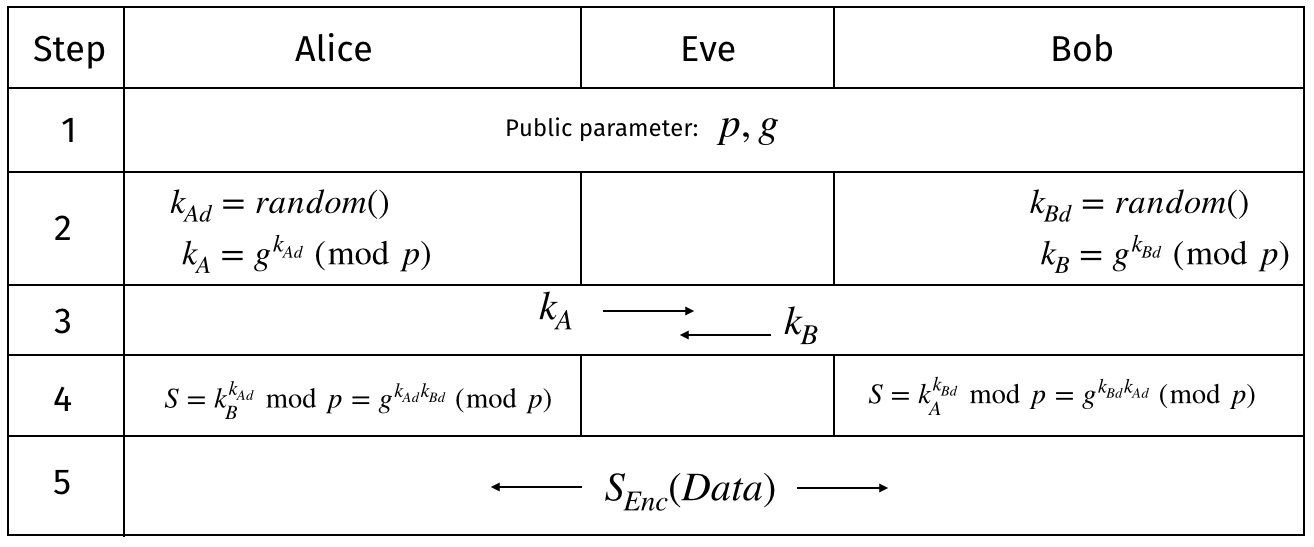
\includegraphics[width=.9\linewidth, height=.67\textheight, keepaspectratio]{Figures/DHKE}
	\caption{Exchanging shared secret key using DH-key exchange.}
	\label{fig_DHKE}
\end{figure}

Rivest, Shamir, and Adleman (RSA) realized this protocol in 1977 and published their magnum opus which is widely known as RSA cryptosystem \cite{rivest1978method}. 
The security of the RSA depends on the difficulty of factorization of a larger integer into its two prime factors and the trapdoor permutation for encryption.
Let us denote two large primes $p$ and $q$ (in practice about 1000-bit).
It is easy to calculate their product to get $n = pq$.
The reverse process that is for a given integer $n$ it will be arduous to retain $p$ and $q$.
Using the state-of-the-art integer factoring algorithm \textit{general number field sieve }(GNFS), it will take approximately $2^{90}$ basic operation to factor a 2048-bit integer.
After more than 40 years of the RSA breakthrough, it is still standing as an epitome of public key cryptography.
Besides encryption, RSA also enables \textit{digital signature }where the sender uses his private key to sign a message, and the receiver verifies the signature by the senders public key. 
Verification of a digitally signed message gives the receiver the confidence that a senders private key is tied to his public key.
It is done to prevent forgery and holds \textit{Non-repudiation} property.

In the mid 80's the independent work of Miller \cite{C:Miller85} and Koblitz \cite{koblitz1987elliptic} began the journey of elliptic curve cryptosystems (ECC). 
The security of elliptic curve cryptography protocols depends on the difficulty to solve elliptic curve discrete logarithm problem.
The mathematical details of this problem appear in Chapter 2. %TODO
ECC provides a shorter key length for the same level of security than RSA which makes ECC  popular among the researchers. 
Compared to RSA, ECC has other advantages. 
While RSA provides encryption and digital signature; ECC has a family of algorithms for encryption, signature, key agreement and some advanced high-level cryptographic protocols such as ID-based encryption \cite{AC:BonLynSha01}, where user's unique ID, e.g. email address, can be used as a public key. 
The high-level cryptographic functionalities are provided by paring over elliptic curves \cite{book_GPCMrabet2016} which brings a new paradigm in cryptography called pairing-based cryptography.

\subsection{Pairing-Based Cryptography}
\label{ch1_subsec_pbc}
Since the inception by Sakai et al. \cite{sakai2000cryptosystems}, pairing-based cryptography has gained much attention to cryptographic researchers as well as  to mathematicians. It gives flexibility to protocol researcher to innovate applications with provable security and at the same time to mathematicians and cryptography engineers to find efficient algorithms to make pairing implementation more efficient and practical.

Generally, a pairing is a bilinear map $e$ typically defined as  $\g1 \times \g2 \to \g3$, where $\g1$ and $\g2$ are additive cyclic sub-groups of  order $r$  on a certain elliptic curve $E$ over a finite extension field $\FPK$ and $\g3$ is a multiplicative cyclic group of order $r$ in $\mF{p}{k}$.
Let $E(\Fp)$ be the set of rational points over the prime field $\Fp$ which forms an additive Abelian group together with the point at infinity $\cal{O}$. The total number of rational points is denoted as $\#E(\Fp)$. Here, the order $r$ is a large prime number such that $r | \#E(\Fp)$ and gcd$(r,p)=1$. The embedding degree $k$ is the smallest positive integer such that $r | (p^k -1)$.
Two fundamental properties of pairing are
\begin{itemize}
	\item bilinearity is such that $\forall P_i \in \g1$ and $\forall Q_i \in \g2$, where $i= 1, 2$, then $e(Q_1+Q_2,P_1) = e(Q_1,P_1). e(Q_2,P_1)$ and $e(Q_1,P_1+P_2) = e(Q_1,P_1). e(Q_1,P_2)$,
	\item and $e$ is non-degenerate means $\forall P \in \g1$ there is a $Q \in \g2$ such that  $e(Q,P) \neq 1$ and $\forall Q \in \g2$ there is a $P \in \g1$ such that $e(P,Q) \neq 1$.
\end{itemize}
Such properties allows researchers to come up with various cryptographic applications including ID-based encryption \cite{C:BonFra01}, group signature authentication \cite{C:BonBoySha04}, and functional encryption \cite{C:OkaTak10}.  However, the security of pairing-based cryptosystems depends  on 
\begin{itemize}
	\item  the difficulty of solving elliptic curve discrete logarithm problem (ECDLP) in the groups of order $r$ over $\Fp$,
	\item  the infeasibility of solving the discrete logarithm problem (DLP) in the multiplicative group $\g3 \in \mF{p}{k}$,
	\item and the difficulty of pairing inversion.
\end{itemize}
To maintain the same security level in both groups, the size of the order $r$ and extension field $p^k$ is chosen accordingly. If the desired security level is $\delta$ then $\log_2 r  \geq 2\delta$ is desirable due to Pollard's rho algorithm \cite{1978-pollard-kangaroo}.  For efficient pairing, the ratio $\rho = \log_2 p^k/ \log_2 r \approx 1$,   is expected (usually  $1\leq  \rho  \leq 2$). In practice, elliptic curves with small embedding degrees $k$ and large $r$ are selected and commonly are knows as ``pairing-friendly" elliptic curves.

Galbraith et al. \cite{galbraith2008pairings} have classified pairings as three major categories based on the underlying group's structure as 
\begin{itemize}
	\item Type 1, where $\g1 = \g2$, also known as symmetric pairing. 
	\item Type 2, where $\g1 \neq \g2$, known as asymmetric pairing. There exists an efficiently computable isomorphism $\psi : \g2 \to \g1$ but none in reverse direction.
	\item Type 3, which is also asymmetric pairing, i.e., $\g1 \neq \g2$. But no efficiently computable isomorphism is known in either direction  between $\g1$ and $\g2$.
\end{itemize}


%This thesis chooses one of the Type 3 variants of pairing named as Optimal-Ate \cite{DBLP:journals/tit/Vercauteren10} with Kachisa-Schaefer-Scott (KSS) \cite{EPRINT:KacSchSco07} pairing-friendly curve of embedding degree $k=16$. 
%Few previous works have been done on this  curve. 
%Zhang et al. \cite{INDOCRYPT:ZhaLin12} have shown the computational estimation of the Miller's loop and proposed efficient final exponentiation for 192-bit security level in the context of Optimal-Ate pairing over KSS-16 curve. 
%A few years later Ghammam et al. \cite{EPRINT:GhaFou16b} have shown that KSS-16 is the best suited for multi-pairing (i.e., the product and/or the quotient) when the number of pairing is more than two. 
%Ghammam et al. \cite{EPRINT:GhaFou16b} also corrected the flaws of proposed final exponentiation algorithm by Zhang et al. \cite{INDOCRYPT:ZhaLin12} and proposed a new one and showed the vulnerability of Zhang's parameter settings against small subgroup attack. 
%The recent development of NFS by Kim and Barbulescu \cite{C:KimBar16} requires updating the parameter selection for all the existing pairings over the well known pairing-friendly curve families such as BN \cite{SAC:BarNae05}, BLS \cite{EPRINT:FreScoTes06} and KSS \cite{EPRINT:KacSchSco07}.
%The most recent study by Barbulescu et al. \cite{EPRINT:BarDuq17} have shown the security estimation of the current parameter settings used in well-studied curves and proposed new parameters, resistant to small subgroup attack.
%
%Barbulescu and Duquesne's study finds that the current parameter settings for 128-bit security level on BN-curve studied in literature can withstand for 100-bit security. 
%Moreover, they proposed that BLS-12 and surprisingly KSS-16 are the most efficient choice for Optimal-Ate pairing at the 128-bit security level. Therefore, the authors focus on the efficient implementation of the less studied KSS-16 curve for Optimal-Ate pairing by applying the most recent parameters.
%Mori et al. \cite{PAIRING:MANS13} and Khandaker et al. \cite{ICISC:KONSD16} have shown a specific type of sparse multiplication for BN and KSS-18 curve respectively where both of the curves supports sextic twist. 
%The authors have extended the previous works for quartic twisted KSS-16 curve and derived pseudo-8 sparse multiplication for line evaluation step in the Miller's algorithm. 
%As a consequence, the authors made the choice to concentrate on Miller's algorithm's execution time and computational complexity to verify the claim of \cite{EPRINT:BarDuq17}.
%The implementation shows that Miller's algorithm time has a tiny difference between KSS-16 and BLS-12 curves. However, they both are more efficient and faster than BN curve. 
\section{Motivation}
\label{ch1_sec_motivation}

This section outlines the overall motivation behind the undertaken works.
In this course, some mathematical notations will appear without detailed definitions.
The subsequent chapters will define them with further elaboration.
Let us consider the following two cases.

\subsection*{Case 1: IoT Security}
Human civilization is moving to a direction where data generated from the devices used in our daily life will define how smart our society will be.
In technical jargon, we define that IoT (Internet of Things) era controlled by Data Science.
Some data can be mundane with no purpose, and some data can be extraordinarily important.
Let us imagine a case where the adversary takes controls heartbeat monitor sensor of our smartwatch or control sensors of a self-driving car.
The outcome of the damage is unimaginable. 
There is no alternative to protect these data from unwanted access.
The challenge is, most of the IoT devices are equipped with small sensors.
Such devices are computationally resource constrained.
In some devices, it is somewhat impractical to generate key pairs for widely practiced security protocols.
There are several innovative solutions such as Identity-based encryption that can use device's unique ID as a key.
The applications mentioned above stand on a compelling branch of cryptography named \textit{pairing-based cryptography over elliptic curve}.


\subsection*{Case 1: Security of Medical Data in Cloud}
Modern medical diagnosis depends on medical examination that produces a vast amount of data ranges from patients personal information to diagnosis reports and images.
Most of the data are stored in large cloud-based databases. 
For the privacy of the patient, they should be encrypted before stored.
By analyzing such medical data, it is possible to predict the probability of a patient's vulnerability to a particular disease. 
However, it is not always the doctor who examined the patient can do that.
Sometimes third-party researchers are interested in such data-set. 
However, the identity of the patient should not be obtained by any third-party using that data. 
One solution for this case is any third party can search data and perform the mathematical operation in the encrypted database without decrypting the data.
This scenario can be realized by using homomorphic encryption which is also powered by pairing-based cryptography.

However, pairing-based cryptography is a complex mathematical process.
To practically apply it, we need to carry out its fundamental algorithms more efficiently.
In this thesis, our objective is to improve and find out more efficient algorithms that can realize high-level of security protocols.

\section{Our Contribution}
\label{ch1_sec_contribution}
As discusses above, pairing is a bilinear map from two groups $\mathbb{G}_1$ and $\mathbb{G}_2$ to a group $\mathbb{G}_3$, where they have respectively same prime order $r$.
In detail, $\mathbb{G}_1$ and $\mathbb{G}_2$ respectively becomes a subgroup in an elliptic curve group $E(\F{q}{})$ and $E(\F{q}{k})$, and $\mathbb{G}_3$ becomes a subgroup in $\F{q}{k}$, where $q$ is a power of $p$ and an extension degree $k$ is especially called the {\it embedding degree}.

In pairing-based cryptography, there exists several predominant operations which are the bottleneck for any pairing-based protocols.
These operations are Miller's algorithm, final exponentiation in $\mathbb{G}_3$, scalar multiplications in $\mathbb{G}_1$ and $\mathbb{G}_2$, and exponentiation in $\mathbb{G}_3$.
The calculation costs of pairing and scalar multiplication in $\g{2}$ are the significant costs among the operations required for pairing-based cryptographies.
Therefore, efficient Miller's algorithm and scalar multiplications in $\mathbb{G}_2$ can reduce the total cost of pairing-based cryptography.
In this work, we focus on these operations especially Miller's algorithm and scalar multiplications in $\mathbb{G}_2$.
	
In this thesis, we focus on Type 3 pairing that is asymmetric pairing such as Ate \cite{EPRINT:MKHO07} and Optimal-Ate \cite{DBLP:journals/tit/Vercauteren10} pairing.
Therefore, we have not efficient homomorphic map from $\g{1}$ to $\g{2}$. 
Generally, in asymmetric pairing the scalar multiplication is carried out over efficiently calculable group $\g{1}$ and then the result is mapped to $\g{2}$.

The {\it embedding degree} is an important parameter that determines the security level of pairing-based cryptographies.
Therefore, to achieve efficient pairing on ordinary curves whose {\it embedding degree} are flexibly selectable are required.
This thesis targets Ate and {\it twisted} Ate pairings because they are efficiently calculated on normal pairing-friendly curve Kachisa-Schaefer-Scott (KSS) \cite{EPRINT:KacSchSco07}.
Ate and Optimal-Ate are use calculated over certain elliptic curve groups $\g{1}$ and $\g{2}$.
In this thesis, we accelerate scalar multiplications in $\g{2}$ group which can be extended in $\g{1}$

In the case of scalar multiplication, we reduce the number of elliptic curve doubling by decomposing a scalar with a key relation for KSS curves.
Besides, we proposed state-of-the-art Miller's algorithm calculation at the 128-bit security level.

Our proposed methods can substantially improve pairing calculation.
Therefore, our research contributes to committing high-level security for sophisticated protocols, e.g. ID-based or Homomorphic encryption.

\section{Thesis Outline}
\label{ch1_sec_outline}
This thesis is organized as follows: 

In Chapter 2, we briefly discuss the mathematical concepts that are related to understanding the concepts of this thesis.
We also define the pairing in general. 
Besides, a target class of pairing-friendly elliptic curves is shown.

Chapter 3 proposes an efficient Optimal-Ate pairing for KSS-18 curve. 
We improved the Miller's algorithm of Optimal-Ate pairing by proposing \textit{pseudo 12-sparse multiplication} multiplication.
In order to evaluate our theoretic proposal, we also include some experimental results with recommended parameter settings.

Chapter 4 proposes a technique that will accelerate scalar multiplications in $\g{2}$ over KSS-18 curve. 
It is crucial to derive efficiently computable endomorphisms for accelerating scalar multiplication.
The target $\g{2}$ group has a property that specific scalar multiplication can utilize  Frobenius endomorphism that is efficiently computable.
Focusing on this property, we derive an essential relation available for scalar multiplication in $\g{2}$ from the structural properties of target elliptic curve.
Then, using the relation, efficient scalar multiplication is proposed together with multi-scalar multiplication.
Besides, from the experimental results, we show that the proposed scalar multiplication is about 60 times faster than the conventional method.  

In chapter 5, we derived twist property for target elliptic curves for 192-bit security level and compared their performances concerning scalar multiplication.
This thesis shows that sextic twist over KSS-18 curve has an advantage over quartic twist in KSS-16 curve.

Chapter 6, shows the state-of-the-art improvement of Optimal-Ate pairing over KSS-16 curve at the 128-bit security level.
We adopted the most recent parameter and theoretically derived most efficient pairing calculation.
Besides, we also showed experimental implementation and compared our result with other pairing-friendly curves.


In Chapter 7, we opt to further accelerate the work of chapter 6 by improving the finite field arithmetic using cyclic vector multiplication algorithm.
We showed comparative results between chapter 6's proposal and this. 
We also showed memory optimization currently exists final exponentiation algorithm.

Chapter 8 shows the   $\g{2}$  scalar multiplication with by applying different dimension of GLV decomposition.
We showed theoretical and experimental result and showed that 4-dimension is optimal for efficient scalar multiplication in  $\g{2}$ in KSS-16 curve.

Finally, Chapter 9 concludes this thesis.

	


%\extraPartText{Always be friendly to ducks, capybaras and wombats.}
%\part{Basic Math}
%
\chapter{Fundamental Mathematics and Notation}
\label{chap:fundamentals} 
It is necessary to recall some fundamental mathematical concept to understand the subsequent chapters and introduce the notations used in the thesis.
This chapter introduces the essential mathematical backgrounds that are directly relevant to the contents of this thesis to help readers to a clear understanding of the subsequent chapters.
The theoretical discussion will often appear with minimal definition and citation of the details works since details discussion is beyond the scope of this thesis.
For more details of the topics discussed in this chapter we refer to \cite{lidl_niederreiter_1996, book_HFFMullen2013}.
As an additional purpose, this chapter specifies most of the notations that will appear in the upcoming chapters.
% For referencing the chapter elsewhere, use \ref{Chapter1} 

Cryptography deals with numbers mostly integers.
To understand modern cryptography  it is essential to have a good understanding of the  underlying mathematical concepts. 
The following concepts is the basic for the discussion of the subsequent chapters.

\section{Modular Arithmetic}
\label{sec:chap:fund:modular_arithm} 
 Modular arithmetic is the fundamental tool for modern cryptography specially public key cryptosystems.
\begin{definition}[Modular Arithmetic\index{modulus}]
	Let  $p$ be a positive integer named as the modulus \index{modulus} and  $a$ and $b$  are two arbitrary integers. 
	If  $p$ divides $b-a$  then we can write
	 $$ a \equiv b ~(\bmod ~p)$$
	 and express as $a$ and $b$ are congruent modulo $p$.
\end{definition}
\begin{example}
	Let, $p =7$, $a=19$ and $b=5$ then 
	$19  \equiv  5 ~(\bmod ~7) $.
\end{example}

\begin{example}
	Let, $p =7$, $a=-17$  and $b=11$. Then $-17  ~(\bmod ~7)  = 4$ and $11 ~(\bmod ~7) = 4$. 
	We can write 
	$$-17  \equiv  11 ~(\bmod ~7) $$ 
	and usually express $-17$ and $11$ are congruent modulo $7$.
\end{example}

\section{Group, Ring, Field}
\label{sec:chap:fund:group}
\subsection{Group}
The concept of group \index{group} is very fundamental for understanding cryptography. It is an algebraic system defined as follows.
\begin{definition}[Group\index{group}]
A group \index{group} is a non empty set $\mathbb{G}$ with a binary operation $\circ$ on its elements denoted as  $\langle\mathbb{G}\index{group},\circ\rangle$,  sometimes denoted by   $\mathbb{G}$ only, which satisfies the following axioms.
\begin{quote}
	\begin{description}
		\item[Closure] The group is closed under the operation $\circ$, i.e.  $\forall a \in\mathbb{G}$, and $\forall b \in\mathbb{G}$ the result of $ (a\circ b) = c \in \mathbb{G}$. \footnote{$\forall$ symbol bears is usual notation \textit{"for all"} }
		
		\item[Identity element] There exist an \textbf{identity element \index{Identity element}} $e$ also know as \textit{neutral element} or \textit{unit element} in $\mathbb{G}$ such that $\forall a \in\mathbb{G} \index{group}$,  $a\circ e = e\circ a = a$.
		
		\item[Inverse element] For ${\forall}a \in\mathbb{G}\index{group}$, there exists an element $b\in\mathbb{G}\index{group}$ such that $a\circ b=e=b\circ a$, where $b$ is called inverse element of $a$.
		
		\item[Associativity] Elements in  group $\mathbb{G}$ should follow associativity. i.e. $(a\circ b)\circ c=a\circ (b\circ c)$ for all $ a,b,c\in\mathbb{G}\index{group}$.
		
\end{description}
\end{quote}
\end{definition}

\begin{definition}[Commutative Group\index{group}] \hspace{0em}
\begin{quote}\begin{description}
A group \index{group} $\mathbb{G}\index{group}$ will be commutative if $a\circ b=b\circ a$ for all $a,b \in\mathbb{G}\index{group}$.
\end{description}\end{quote}
\qed
\end{definition}
A commutative group is also called \textit{abelian} group.

\begin{example} \label{example_group}
 The set of integers $\mathbb{Z}$ forms a group under the group operation of addition $+$ denoted as $(\mathbb{Z},+)$. $0$ is the identity element of the group.
\end{example}
\begin{example}\label{example_notgroup}
	 The set of positive integers $\mathbb{N}$ under addition does not form a group since elements have not inverse.
\end{example}
%For example, the algebraic system $\langle\mathbb{Z},+\rangle$ is an infinite commutative group\index{group}, where $\mathbb Z$ is the integer set and $+$ means the ordinary addition for integers. For a finite group\index{group}, its order\index{group order} is defined as follows.
\begin{definition}[Order of a Group\index{group}]\hspace{0em}
The order of a group $\mathbb{G}$ \index{group order} often denoted as $\#\mathbb{G}\index{group}$ is the number of elements in the group\index{group} $\mathbb{G}\index{group}$.
\qed
\end{definition}

\begin{remark}
	 Groups order can be finite and infinite. In example \ref{example_group}, $(\mathbb{Z},+)$ has infinite order.
\end{remark}

\begin{definition}[Order of group element\index{order of element}]
	For an element $a\in\mathbb{G}\index{group}$, the smallest positive integer $m$ such that $a^{m}=e$ is called the order\index{order} of $a$, where $e$ is the identity element in $\mathbb{G}\index{group}$.
	\qed
\end{definition}

\begin{example}{Finite group:  \index{finite group} } \label{definition_finite_group}
As shown in example \ref{example_notgroup}, the set $\mathbb{N}$ under addition does not form a group 
since it does not satisfy the group\index{group} axioms. 
Let us consider a set $\mathbb{N}_{n}$ under the operation $\mod n$  such that 
$$ \mathbb{N}_{n} = \{0,1,2,3, \cdots, n-1\}$$
where $n \in \mathbb{N}$.
It means $\mathbb{N}_{n}$ is the set of remainders under ``$\bmod\ n$''.
Recall the modular arithmetic that 
$$a+b\equiv c\ \ \bmod n\hspace{3em}a,b\in \mathbb{N}_{n},\label{Sum Definition}$$
 means $c$ is  associated to a remainder on division by $n$ when $a+b=c\notin\mathbb{N}_{n}$. 
It makes $c$ belongs to $\mathbb{N}_{n}$ making $( \mathbb{N}_{n},+)$ forming a group\index{group}.
In also includes element $0$ which acts as an identity element.
\end{example}

\begin{definition}[Group generator\index{group}]
	For a given group\index{group} $\mathbb{G}\index{group}$ if there is an element $g\in\mathbb{G}\index{group}$ such that for any $a\in\mathbb{G}\index{group}$ there exist an unique integer $i$ with $a=g^{i}$ then $g$ will be called a   generator\index{generator} of  $\mathbb{G}\index{group}$
\qed
\end{definition}

\begin{definition}[Cyclic Group\index{group}]
A group\index{group} $\mathbb{G}\index{group}$ will be {\em cyclic} if there exist at least one generator $g \in \mathbb{G}$. Cyclic group usually expressed as $\mathbb{G} = \langle g \rangle$
 \qed 
\end{definition}

\begin{remark}
	The number of generator in a group $\mathbb{G}\index{group}$ of order $n$ is defined by Euler's totient function $\phi(n)$\footnote{When $n$ is a positive integer, Euler's totient function $\phi(n)=$ number of positive integers less than or equal to $n$ that are co-prime to $n$}.
	If $n$ is a prime $p$ then the  group $\mathbb{G}$ will be called prime order group and it will have $\phi(p) = p-1$ generators.
\end{remark}

\begin{definition}[Cyclic Group\index{group}]
	A group\index{group} $\mathbb{G}\index{group}$ will be {\em cyclic} if there exist at least one generator $g \in \mathbb{G}$. Cyclic group usually expressed as $\mathbb{G} = \langle g \rangle$ 
	\qed 
\end{definition}

In this case we use the notation $\langle\mathbb{G}\index{group},\circ\rangle$,  there exists some ambiguity which operation we consider.
Therefore, the following two types of group nations are very common in literature.

\begin{definition}[Additive group\index{additive group}]
A cyclic group is called \textit{additive} if we tend to write its group operation in the same way we do additions, that is 
$$f = g + x$$ 
can also appear as $[x]g$ meaning applying $x -1$ times addition operator $+$ on $g$.
It is also common to write as $x \cdot g$.
For example, $1$ is one of generators in group $(\mathbb{Z}_5, + )$ under addition modular $5$, then $1 \cdot 4$ can be written as $$ 4 = 1+ 1+ 1+1.$$
\qed
 \end{definition}

\begin{definition}[Multiplicative group\index{multiplicative group}]
	A cyclic group is called \textit{multiplicative} if we tend to write its group operation in the same way we do multiplication, that is 
	$$f =  g \cdot x ~\text{or}~ f = g^x$$ 
	\qed
\end{definition}

\begin{remark}
	In both notation the $x$  is an integer called the \textit{discrete logarithm} of $h$ to the base $g$.
\end{remark}
\begin{remark}
	Unless otherwise stated, through out this thesis we will use the $xg$ notation for ordinary addition e.g. $a+a=2a$ and $a+a+a=3a$ and for multiplicative notation, these will denoted by $a^2$, $a^3$.
\end{remark}

From the definition cyclic group, it can be see visualized that any elements in cyclic a group\index{cyclic group} are generated with iterative operations of generator\index{generator} $g$. 
\fgref{Cyclic group} shows this schematically.
\begin{figure}[ht]
\begin{center}
	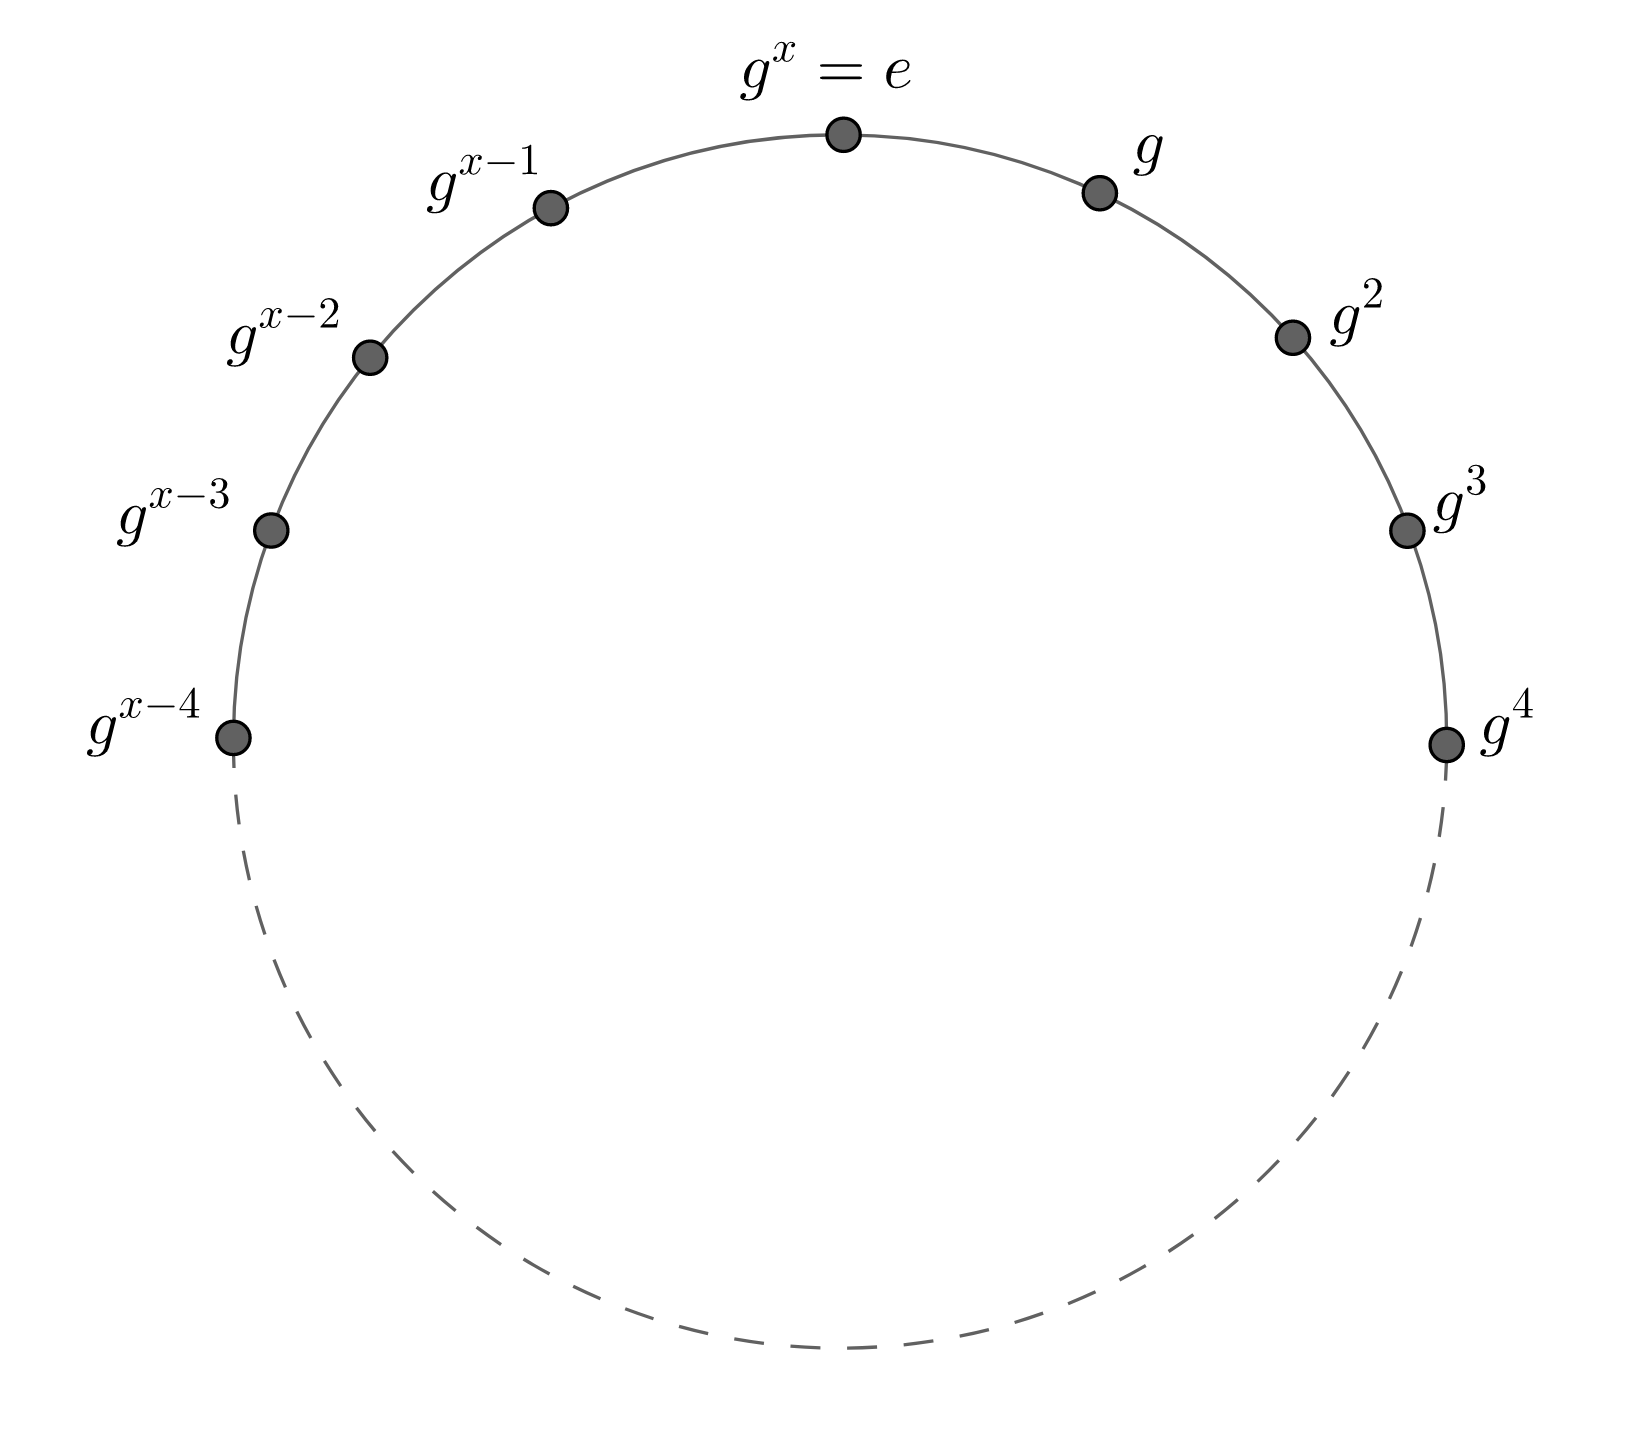
\includegraphics[width=.6\linewidth, height=.67\textheight, keepaspectratio]{Figures/cyclicgroup}
\caption{Cyclic group\index{cyclic group}\index{group}}
\label{Cyclic group}
\end{center}
\end{figure}

A a well known practice of presenting a finite group's\index{group} operation is {\em Cayley table\index{Cayley table}} as shown in example \ref{example_Cayleytable}.
Cayley table\index{Cayley table} shows all possible group operation that can be performed in a finite group.

\begin{example} \label{example_Cayleytable}
	The Cayley table\index{Cayley!Cayley table} for the group\index{group} $\mathbb{Z}_4$ is:
	\begin{center}
		\begin{tabular}{c|cccc}
			$\oplus_4$&\em 0&\em 1&\em 2&\em 3       \\
			\hline
			\em 0&\em 0&\em 1&\em 2&\em 3       \\
			\em 1&\em 1&\em 2&\em 3&\em 0       \\
			\em 2&\em 2&\em 3&\em 0&\em 1       \\
			\em 3&\em 3&\em 0&\em 1&\em 2       \\
		\end{tabular}
	\end{center}
\end{example}
In the above example of group $(\mathbb{Z}_4,+)$, there are $\phi(4)=2$ generators, $3$ and $1$.

\begin{definition}[Subgroup\index{subgroup}]
	Let $\mathbb{H}$ be  a non-empty subset  fo group $\mathbb{G}$, $\mathbb{H}$  will be called subgroup of $\mathbb{G}$ if  $\mathbb{H}$  itself follows group axioms and $\mathbb{H}$ has the same identity element of group $\mathbb{G}$. 
	\qed
\end{definition}

\begin{theorem}[Lagrange's Theorem:]
	Let $\mathbb{G}$ be a finite abelian group and $\mathbb{H}$ is a subgroup of $\mathbb{G}$.  The order of $\mathbb{G}$, $\#\mathbb{G}$ is divisible by the order of subgroup $\mathbb{H}$, $\#\mathbb{H}$ i.e.   $\#\mathbb{H} | \#\mathbb{G}$.
\qed
\end{theorem}

\begin{theorem}[Fermat’s Little Theorem:]
	Let $p$ is a prime and $a \in \mathbb{Z}$, then $$a^p = a ~(\bmod ~p)$$
	\qed
\end{theorem}
Fermat’s \textit{little theorem} is a special case of Lagrange’s theorem.


\subsection{Homomorphism in groups \index{homomorphism}}
Morphisms in groups is often used the research of cryptography and inseparable to for pairing-based cryptography research.
\begin{definition}[Homomorphism\index{rings}]
	Let $(\mathbb{G},\circ)$ and $(\mathbb{G}^{'},\star)$ be two groups with identity elements $e$ and $e'$ respectively.
	A homomorphism  is a map $f$ which preserves the group structure while the elements are mapped from $(\mathbb{G},\circ)$ to $(\mathbb{G}^{'},\star)$.
	\qed
\end{definition}
	A homomorphic map obeys the following conditions:
	\begin{itemize}
		\item $\forall a,b \in \mathbb{G}$, $f(a \circ b) = f(a) \star f(b)$.
		\item  For every $a \in \mathbb{G}$, the inverse map is $f(a^{-1}) = f(a)^{-1}$.
		\item  Identity element mapping also preserves the structure i.e. $f(e) =e'$.
	\end{itemize}

\subsubsection{Types of Homomorphism}
\begin{quote}
	\begin{description}
				\item[Isomorphism \index{Isomorphism}] If element from $\mathbb{G}$  and $\mathbb{G}^{'}$ have bijective relation then $\mathbb{G}$ and $\mathbb{G}^{'}$ are isomorphic to each other.
					
			\item[Endomorphism  \index{Endomorphism}]  If elements from group $(\mathbb{G},\circ)$ is mapped to itself then it is called endomorphism. 
			A frequently used endomorphism in cryptographic algorithms is Frobenius endomorphism. 
			
			\item[Authomorphism  \index{Authomorphism}] If element of a group has both endomorphism and isomorphism then it is called automorphism.
	\end{description}
\end{quote}

\begin{definition}[Kernel\index{kernel}]
	Let $(\mathbb{G},\circ)$ and $(\mathbb{G}^{'},\star)$ be two groups with identity elements $e$ and $e'$ respectively and $f$ is homomorphism from $(\mathbb{G},\circ)$ to $(\mathbb{G}^{'},\star)$.
	The kernel of $f$ is denoted as $\text{Ker}\{f\}$, defined by 
	$$\text{Ker}(f) = \{ a \in \mathbb{G}: f(a) = e'\}$$.
	\qed
\end{definition}

%--------------------------------------
%--------------------------------------
\subsection{Ring}
The concept of \textit{Ring} will not come as frequently as group and field in the subsequent chapters. 
However, it is relevant to define ring to understand the related concept.
\begin{definition}[Ring \index{ring}]
	A \textbf{ring} $\mathbb{R}$ is an algebraic structure with two operations, i.e. addition  $+$ and  multiplication $\cdot$  usually denote as $\mathbb{R},+,\cdot$.
	\begin{itemize}
		\item $\mathbb{R}$ is abelian group under addition operation.
		\item Under multiplication, $\mathbb{R}$ is closed and associative with identity element is $1$.
		\item  Multiplication is distributive over addition: $ \forall a, b, c \in \mathbb{R}: a\cdot (b+c) = a\cdot b + a\cdot c$.
	\end{itemize}
\qed
\end{definition}
If multiplication operation is commutative, $\mathbb{R}$  forms a commutative ring.
%\begin{example}
%	TODO
%\end{example}
\begin{definition}[Multiplicative Inverse Modulo $n$ \index{multiplicative inverse}]
	Let $\mathbb{Z}_n$ be a set under modulo $n$ and $a \in \mathbb{Z}_n$. 
	The multiplicative inverse modulo $n$ of $a$ can be written as  follows:
	$$a\cdot x \equiv  1 \bmod n.$$
The value $x$ is the multiplicative inverse modulo $n$ of $a$, often written as $a^{-1}$.
\qed
\end{definition}
Such value of $x$ only exists if $\text{gcd}(x,n)=1$.
If $n=p$ is a prime then every non-zero element in the set $\mathbb{Z}_p$ will have multiplicative inverse.
Such $(\mathbb{Z}_p,+,\cdot)$ will be a ring and having the above property it will form a field.

\subsection{Field}
\begin{definition}[Field]
	A field $(\f{},+,\cdot)$ is a set that obeys two binary operations denoted by $+$ and $\cdot$, such that:
	\begin{itemize}
%		\begin{itemize}
			\item $\f{}$ is a commutative group with respect to $+$ having identity element $0$.
			
			\item Let ${\f{\,}}^{\ast}\!\!$ is a subset of $\f{}$ having only not-zero element of $\f{}$ i.e. ${\f{}}^{\ast}  = {\f{} ~\backslash \{0\}}$. 
			Then ${\f{\,}}^{\ast}\!\!$ will be called a commutative group respect to multiplication$\cdot$  where every element should have multiplicative inverse in  ${\f{\,}}^{\ast}\!\!$.
			\item For all $a,b,c \in\f{}$  the distributive law will be followed, e.g. $a\cdot(b+c)=a\cdot b+a\cdot c$ and $(b+c)\cdot a=b\cdot a +c\cdot a$.
	\end{itemize}
%\end{itemize}
	\qed
\end{definition}
%In general, the elements $0$ and $1$ denote the unit elements regarding to addition $+$ and multiplication $\cdot$, respectively.
\begin{definition}[Subfield \index{subfield}]\hspace{0em} \label{definition_subfielf}
	Let $\f{1}$ is a subset of field $\f{}$. $\f{1}$ will be called a subfeld if $\f{1}$ itself obeys the laws of field with respect to the field operation inherited from  $\f{}$.
	\qed
\end{definition}
\begin{remark}
	 In Definition \ref{definition_subfielf}, $\f{}$ is called an {\em extension field} of $\f{1}$.
	  If $\f{1}\neq \f{}$, then $\f{1}$ is a {\em proper subfield} of $\f{}$.
 \end{remark}

\begin{definition}[Order of Finite Field \index{order of field}]\hspace{0em}
	The order is the number of elements in $\f{}$. If the order of $\f{}$ is finite, $\f{}$ is called finite field. 
	\qed
\end{definition}
\begin{definition}[Characteristic of Finite Field \index{field characteristics}]\hspace{0em}
	Let $\f{}$ be a field and smallest positive number $n$ such that $n \cdot a= 0$ for every $a\in \f{}$. Such $n$ is called characteristic. If there is no such $n$ in  $\f{}$ then $\f{}$ has characteristics $0$.
	\qed
\end{definition}

Most of the works presented in this dissertation deals with  finite fields only. 
A common property of finite fields often used in cryptographic is fllows:
\begin{theorem}\label{Cyclic Group in Finite Field}
	For every finite field $\f{}$, the multiplicative group $({\f{\,}}^{\ast}\!\!, \cdot)$ is cyclic. 
	\qed
\end{theorem}
%For example, ElGamal encryption \cite{C:ElGamal84} can be defined over multiplicative group of $\f{}$. Its security depends on the difficulty of a problem in $\f{}$ related to computing {\em discrete logarithms}.
%A subset $\mathbb K$ of a field $\f{}$ that is itself a field under the operations of $\f{}$ will be called a {\em subfield} of $\f{}$. In this case, $\f{}$ is called an {\em extension (field)} of $\mathbb K$. If $\mathbb K\neq \f{}$, we say that $\mathbb K$ is a {\em proper subfield} of $\f{}$. Then, {\em prime field} is defined as follows.
\begin{definition}[Prime Field \index{prime field}]
	Let $p$ be a prime. The ring of integers modulo $p$ is  a finite field of characteristics $p$ having field order $p$ denoted as $\f{p}$ is called a prime field.
	 \qed
\end{definition}
\begin{remark}
		A prime field contains no proper subfield.
\end{remark}

\begin{theorem}
	Every finite field has a prime field as a subfield. \qed
\end{theorem}

In this work we classified finite fields into two types, i.e.  prime field $\f{p}$ and its extension field. 
Defined \ref{sec:chap:fund:extenion_field} explains more of extension field.
The prime field $\Fp$ has  the order and characteristic as $p$.
Using the modular arithmetic in the same way as Definition \ref{sec:chap:fund:extenion_field}, we can define fundamental operations of prime field $\Fp=\{0,1,2\cdots,p-1\}$.
The Cayley table will de
\begin{example}The Cayley table for the two operations $+$ and $\cdot$ for elements in $\f{5}$ are as follows:
	\begin{center}
		\begin{tabular}{c|ccccc}
			$+$&\em 0&\em 1&\em 2&\em 3&\em 4       \\
			\hline
			\em 0&\em 0&\em 1&\em 2&\em 3&\em 4       \\
			\em 1&\em 1&\em 2&\em 3&\em 4&\em 0      \\
			\em 2&\em 2&\em 3&\em 4&\em 0&\em 1      \\
			\em 3&\em 3&\em 4&\em 0&\em 1&\em 2      \\
			\em 4&\em 4&\em 0&\em 1&\em 2&\em 3      \\
		\end{tabular}\ \ 
		\begin{tabular}{c|ccccc}
			$\cdot$&\em 0&\em 1&\em 2&\em 3&\em 4       \\
			\hline
			\em 0&\em 0&\em 0&\em 0&\em 0&\em 0       \\
			\em 1&\em 0&\em 1&\em 2&\em 3&\em 4      \\
			\em 2&\em 0&\em 2&\em 4&\em 1&\em 3      \\
			\em 3&\em 0&\em 3&\em 1&\em 4&\em 2      \\
			\em 4&\em 0&\em 4&\em 3&\em 2&\em 1      \\
		\end{tabular}
	\end{center}
\end{example}
As described above, we can define arithmetic operations in $\Fp$ by modular operations ($\bmod\ p$) for integers. However, it does not work in an extension field $\F{p}{m}$. In the next section, arithmetic operations in extension field $\F{p}{m}$ is described in detail.


\section{Extension Field} 
%\label{sec:chap:fund:extenion_field}
\label{sec:chap:fund:extenion_field}
%--------------------------------------
A subset $\F{0}{}$ of a field $\F{}{}$ that is itself a field under the operations of $\F{}{}$ will be called a {\it subfield} of $\F{}{}$.
In this case, $\F{}{}$ is called an {\it extension field} of $\F{0}{}$.
An extension field of a prime field $\F{p}{}$ can be represented as $m$-dimensional vector space that has $m$ elements in $\F{p}{}$.
Let the vector space be the $m$-th extension field, it is denoted by $\F{p}{m}$.
The order of extension fields $\F{p}{m}$ is given as $p^m$. 
In what follows, let $q$ be the power of $p$, the extension field of a prime field $\F{p}{}$ is denoted by $\F{q}{}$.



There are several methods to represent an element in extension fields, such as polynomial basis and normal basis.
In this thesis, we use normal basis.
Let $\omega$ be a root of $m$-th irreducible polynomial over $\F{q}{}$, we consider the following $m$ elements.

\begin{equation}
\omega,\;\omega^q,\;\omega^{q^2},\;\cdots,\;\omega^{q^{m-1}} \nonumber
\end{equation}
All elements in this set are conjugate to each other.
When the set of the conjugates become linearly independent, this is called {\it normal basis}.
Using normal basis, an element $\alpha \in \F{q}{}$ is expressed as a polynomial by  
\begin{equation}
\alpha = a_1 \omega + a_2 \omega^q + a_3 \omega^{q^2} + \cdots + a_m \omega^{q^{m-1}}, 
\end{equation}
where $a_1,\;a_2,\;a_3,\cdots,\;a_m \in \F{q}{}$.

Arithmetic operations in $\F{q}{m}$ are carried out with ordinary addition and multiplication for polynomial and modular reduction by irreducible polynomial.

\section{Frobenius Map}
\label{sec:chap:fund:frobeniusmap}
%--------------------------------------

For any element $\alpha \in \F{q}{m}$, let us consider the following map $\pi_q:\alpha \rightarrow \alpha^q$. 
%$\F{q}{m}$‚Ì”CˆÓ‚ÌŒ³$\alpha$‚ɑ΂µ‚Ä$\pi_q:\alpha \rightarrow \alpha^q$‚Æ‚¢‚¤ŽÊ‘œ‚ðl‚¦‚éD
\begin{eqnarray}
\pi_q(\alpha) &=& \left( a_1 \omega + a_2 \omega^q + a_3 \omega^{q^2} + \cdots + a_m \omega^{q^{m-1}} \right)^q \nonumber \\ 
&=& a_1 \omega^q + a_2 \omega^{q^2} + a_3 \omega^{q^3} + \cdots + a_m \omega^{q^m} \nonumber \\
&=& a_m \omega + a_1 \omega^q + a_2 \omega^{q^2} + \cdots + a_{m-1} \omega^{q^{m-1}}
\end{eqnarray}
Note that the order of $\F{q}{m}^*$ is given by $q^m - 1$, that is,  $\omega^{q^m} = \omega$ is satisfied.
Furthermore, $a^q$ is equal to $a$ for each coefficients $a$.

Therefore, the map $\pi_q(\alpha)$ is efficiently calculated by cyclic shift operations among its basis coefficients, 
which is free from arithmetic operations.
From the computational efficiency, the map $\pi_q$ is especially called Frobenius map.

In ElGamal Encryption, many exponentiations are executed in encryption and decryption processes.
When the exponent is equal to $p$, its calculation cost can be reduced by using Frobenius map.
Therefore, Frobenius map is widely used in the cryptographic application.     

\section{Quadratic Residue/Quadratic Non-residue, \\and Cubic Residue/Cubic Non-residue}
\label{sec:chap:fund:qrqnr}
%--------------------------------------

For any non-zero element $d\in\F{q}{}$, $d$ is called a Quadratic Residue (QR) when $x$ such that $x^2=d$ exists in $\F{q}{}$.
On the other hand, when such an $x$ does not exist in $\F{q}{}$, $d$ is called a Quadratic Non-Residue (QNR).
We can identify whether or not $d$ is a QR by following test.
%$\f{q}$‚Ì”CˆÓ‚Ì”ñ—댳$d$‚ɑ΂µC$x^2=d$‚Æ‚È‚é$x$‚ª$\f{q}$‚É‘¶Ý‚·‚é‚Æ‚«C$d$‚𕽕ûè—]iQuadratic Residue; QRj‚Æ‚¢‚¢C
%‘¶Ý‚µ‚È‚¢‚Æ‚«•½•û”ñè—]iQuadratic Non-Residue; QNRj‚Æ‚¢‚¤D‚»‚Ì”»•Ê‚ÍŽŸŽ®‚É‚æ‚ès‚¦‚éD
\begin{eqnarray}
d^{(q-1)/2} = \left\{
\begin{array}{ll}
1 & \mbox{: QR} \\
-1 & \mbox{: QNR} 
\end{array}
\right.
\end{eqnarray}

All elements in finite fields $\F{q}{}$ of odd characteristics become QR in extension fields $\F{q}{2j}$.
On the other hand, quadratic non-residues also become QNR in $\F{q}{i}$, where $i$ is not divisible by 2.

%%%%%%%%%%%%%%%%%%%%%%%%%%%%%%%%%%%%%%%
\section{Elliptic Curve}
\label{sec:chap:fund:ecc}
In this section, we review elliptic curves and pairings. 

%--------------------------------------
\subsection{Additive Group over Elliptic Curves}
%--------------------------------------

In general, let $p>3$, an elliptic curve $E/\F{p}{}$ over a finite field $\F{p}{}$ is defined as 

\begin{equation}
E/\F{p}{}: y^2=x^3+ax+b,\ 42a^3+27b^2 \neq 0,\ a,b\in \F{p}{}. \label{EC}
\end{equation}

The field that $x$ and $y$ belong to is called the definition field. 
The solutions $(x,y)$ of \eqref{EC} is called rational points.
$E(\F{q}{})$ that is the set of rational points on the curve, including the {\it point at infinity} $\mathcal{O}$, forms an additive abelian group. 
The {\it point at infinity} works as an unity element in $E(\F{q}{})$.
When the definition field is $\F{q}{m}$, we denote the additive group by $E(\F{q}{m})$.

For rational points $P_1(x_1,y_1)$, $P_2(x_2,y_2)$ $\in E(\F{q}{})$, the elliptic curve addition $P_3(x_3,y_3)=P_1+P_2$ is defined as follows.
\begin{eqnarray*}
	\lambda &=& \left\{ \begin{array}{ll}
		{\displaystyle \frac{y_2-y_1}{x_2-x_1}} & P_1\neq P_2,\ x_1\neq x_2 \\
		& \\
		{\displaystyle \frac{3x_1^2+a}{2y_1}} & P_1=P_2 \\
		
	\end{array} \right.\\
	x_3 &=& \lambda^3-x_1-x_2\\
	y_3 &=& (x_1-x_3)\lambda-y_1
\end{eqnarray*} 
%In the case of $P_1=P_2$, the addition is especially called elliptic curve doubling. 
$\lambda$ is the tangent at the point on the curve and $\cal O$ is the additive unity in $E(\f{p})$.
In what follows, If $P_1 \neq P_2$ then $P_1+P_2$ is called elliptic curve addition (ECA). 
If $P_1=P_2$ then $P_1+P_2=2P_1$, which is known as elliptic curve doubling (ECD). 
%Let $\#E(\F{p}{})$ be its order, consider a large prime $r$ that divides $\#E(\F{p}{})$. %The smallest positive integer $k$ such that $r$ divides $p^k-1$ is called {\it embedding degree}. One can consider pairings such as Tate and Ate pairings by using $E(\F{p}{k})$. 

Let a rational point $P(x,y)$, an inverse point $-P$ is given by $-P(x, -y)$. 
Elliptic curve cryptographies is constructed on elliptic curve groups $E(\F{q}{})$.



Let $\#E(\F{p}{})$ be the order of $E(\F{p}{})$, it is given as
\begin{equation}
\#E(\F{p}{})=p+1-t, %abel{order}
\end{equation}
where $t$ is the Frobenius trace of $E(\F{p}{})$. 

From Hasse's theorem, $t$ satisfies
\begin{equation}
|t| \leq 2\sqrt{p}.
\end{equation}

\subsection{Scalar Multiplication in Elliptic Curve}
\label{sec:chap:fund:scm}
Let $[s]P$ denote the $(s-1)$-times addition of a rational point $P$ as, 
\begin{equation}
[s]P = \sum_{i = 0}^{s-1}{P}.
\end{equation}
This operation is called a scalar multiplication.
As a general approach for accelerating a scalar multiplication, the binary method is the most widely used.

\paragraph{Binary method}
\label{sec:chap:fund:binscm}
The binary method is an extensively applied method for calculating the elliptic curve scalar multiplication. 
 The pseudo code of left-to-right binary scalar multiplication algorithm is shown in \algref{alg:binary_scm_chap_fundamental}. 
 This algorithm scans the bits of scalar $s$ from the  most significant bit to the least significant bit. When $s[i] = 1$, it  performs ECA and ECD otherwise only ECD is calculated. 
 The binary method iterates elliptic curve doublings and elliptic curve additions using binary representation of scalar.
 A scalar multiplication needs $\lfloor \log_2 s\rfloor$ elliptic curve doublings and $\lfloor \log_2 s\rfloor/2$ elliptic curve additions on average.
  This method is easy to implement but the important drawback of this method is not resistant to \textit{side channel attack} \cite{C:Kocher96}.  

\begin{algorithm}[ht]
	\caption{Left-to-right binary algorithm for elliptic curve scalar multiplication}
	\label{alg:binary_scm_chap_fundamental}
	\DontPrintSemicolon
%	\hspace{-3ex}
	\KwIn{ $P$, $s$}
%	\hspace{-3ex}
	\KwOut{$[s]P$} %output
	 $T$ $ \leftarrow$ $0$ \;
	 \For{$i = \lfloor \log_2 s \rfloor$ {\bf to} $0$} {\;
				$T \leftarrow T  + T$\;
		    \If{ $s[i] = 1$}{
			      $ T \leftarrow T + P$\;
	} }
	 \text{return} $T$\;
\end{algorithm}

\paragraph{Montgomery ladder method}
\label{sec:chap:fund:montscm}
Montgomery ladder algorithm is said to be resistant to \textit{side channel attack}. Such resistance comes by paying tolls as calculation overhead which slows down this method than binary method.  \algref{alg:mont_scm_chap_fundamental} shows the Montgomery ladder algorithm for scalar multiplication. Montgomery ladder has some similarity with binary method except in each iteration it performs ECA and ECD. 

\begin{algorithm}[ht]
	\caption{Montgomery ladder algorithm for elliptic curve scalar multiplication}
	\label{alg:mont_scm_chap_fundamental}
	\DontPrintSemicolon
%	\hspace{-3ex}
	\KwIn{ A point $P$,  an integer $s $}
%	\hspace{-3ex}
	\KwOut{$[s]P$} %output
	 $T_0$ $ \leftarrow$ $0$, $T_1$ $\leftarrow$ $P$ \;
	 \For{$i = \lfloor \log_2 s \rfloor$ {\bf to} $0$} {\;
		  \If{ $s[i] =1$}{
			         $ T_0 \leftarrow T_0 + T_1$\;
			     $T_1 \leftarrow T_1 + T_1$\;
		}
		        {\ElseIf{$s[i] = 0$}{ 
				      $T_1 \leftarrow T_0 + T_1$\;
				  		 $T_0 \leftarrow T_0 + T_0$\;}
		}
	}
	 \text{return} $T_0$\;
\end{algorithm}

\paragraph{Sliding-window Method}
\label{sec:chap:fund:swscm}
Sliding-window \cite{DBLP:reference/crc/2005ehcc} algorithm is also resistant to \textit{side channel attack} and at the same  time it is faster than Montgomery ladder. In this method the scalar $s$ is processed in blocks of length $w$, known as window size. \algref{alg:sw_scm_chap_fundamental} shows the sliding-window algorithm for scalar multiplication.

\begin{algorithm}[ht]
	\caption{Sliding window algorithm for elliptic curve scalar multiplication}
	\label{alg:sw_scm_chap_fundamental}
	\DontPrintSemicolon
%	\hspace{-3ex}
	\KwIn{ A point $P$,  an integer $s = \sum_{j=0}^{l-1} s_j2^{j} $, $s_j \in \left\lbrace 0,1 \right\rbrace$, window size $w \geq 1$} 
%	\hspace{-3ex}
	\KwOut{Q = $[s]P$} 
	\textit{Pre-computation.} \; 
	 $P_1\leftarrow P$, $P_2 \leftarrow [2]P$ \;
	 \For{$i = 1$ {\bf to} $2^{w-1}-1$} { $P_{2i+1} \leftarrow P_{2i-1} + P_2$}\;
	 $j \leftarrow l-1$, $Q \leftarrow \cal{O}.$\;
	\textit{Main loop.}\;
	 \While{$j \geq 0$} {\;
		 \If{ $s_j =0$}{
			$Q \leftarrow [2]Q$, $j \leftarrow j-1$\;
		}
		            \Else{\;
			 Let $t$ be the least ineger such that \;
			$j - t+1 \leq w$ and $s_t =1$\;
			 $h_j \leftarrow (s_js_{j-1} \cdots s_t)_2$\;
			 $Q \leftarrow [2^{j-t+1}]Q +P_{h_j}$      \;      
			 $j \leftarrow t-1$ \;
		}
	}
	 return $Q$
\end{algorithm}



%In this paper, the set of rational points $P\in E(\F{q}{})$ satisfying $[r]P=\mathcal{O}$ is denoted by $E(\F{q}{})[r]$.
%For two points $P$ and $R$ such that $[s]P=R$, the problem of solving $s$ is called elliptic curve discrete logarithm problem (ECDLP) and the security of ECC relies on the difficulty of ECDLP.

%\begin{figure}[ht]
%	\begin{center}
%		\special{pn 10}%
%		\special{ar 3150 950 700 700 0.1200000 0.14959965}
%		\special{ar 3150 950 700 700 0.2991993 0.44879895}
%		\special{ar 3150 950 700 700 0.5983986 0.74799825}
%		\special{ar 3150 950 700 700 0.8975979 1.04719755}
%		\special{ar 3150 950 700 700 1.1967972 1.34639685}
%		\special{ar 3150 950 700 700 1.4959965 1.64559615}
%		\special{ar 3150 950 700 700 1.7951958 1.94479545}
%		\special{ar 3150 950 700 700 2.0943951 2.24399475}
%		\special{ar 3150 950 700 700 2.3935944 2.54319405}
%		\special{ar 3150 950 700 700 2.6927937 2.84239335}
%		\special{ar 3150 950 700 700 2.9919930 3.02159265}
%		\special{ar 3850 950 80 80 0.000000000 6.283185304}
%		\special{ar 2450 950 80 80 0.000000000 6.283185304}
%		\special{ar 3150 250 80 80 0.000000000 6.283185304}
%		\special{ar 3500 355 80 80 0.000000000 6.283185304}
%		\special{ar 3745 600 80 80 0.000000000 6.283185304}
%		\special{ar 2555 600 80 80 0.000000000 6.283185304}
%		\special{ar 2800 355 80 80 0.000000000 6.283185304}
%		\special{ar 3150 950 700 700 3.261 3.555}
%		\special{ar 3150 950 700 700 3.79 4.065}
%		\special{ar 3150 950 700 700 4.3 4.591}
%		\special{ar 3150 950 700 700 4.83 5.122}
%		\special{ar 3150 950 700 700 5.365 5.63}
%		\special{ar 3150 950 700 700 5.87 6.165}
%		\begin{picture}(150,120)%
%		\put(50,115){$[\#E]P=\Inf$}
%		\put(110,100){$P$}
%		\put(128,80){$[2]P$}
%		\put(136,54){$[3]P$}
%		\put(-40,54){$[\#E-3]P$}
%		\put(-30,80){$[\#E-2]P$}
%		\put(-10,98){$[\#E-1]P$}
%		\end{picture}%
%	\end{center}
%	\caption{An image of elliptic curve group\index{cyclic group}\index{group}}
%	\label{fig:ECG}
%\end{figure}

%--------------------------------------
\subsection{Frobenius Map on Elliptic Curve Groups}
%--------------------------------------
In this section, we introduce Frobenius map for a rational point in $E(\F{q}{})$.
For any rational point $P=(x, y)$, Frobenius map $\phi$ is given by $\phi:P(x, y) \rightarrow ({x}^q, {y}^q)$.
Then, the following relation holds for any rational points in $E(\F{q}{})$ with regard to Frobenius map.
\begin{equation*}
\left(\phi^{2}-[t]\phi+[q]\right)P=\mathcal{O}.
\end{equation*}
Thus, we have
\begin{equation}
[q]P=\left([t]\phi-\phi^2\right)P. \label{frobscm}
\end{equation}
From Hasse's theorem, note the bit-size of Frobenius trace $t$ is about a half of the characteristic $p$. 
Using \eqref{frobscm}, we can efficiently calculate scalar multiplication \cite{C:Koblitz91}.
 
%\part{Works}
\chapter{ICCE-TW 2016} 
\chapter{ICCE-TW 2016} 

In elliptic curve cryptography (ECC), a scalar multiplication for rational point is the most time consuming operation. This paper proposes an efficient calculation for a scalar multiplication by applying Frobenious Mapping. Particularly, this paper deals with  Barreto-Naehrig curve defined over extension field $\F{q}{2}$, where $q=p^6$ and $p$ is a large prime.

%Scalar multiplication of rational points on elliptic curve (EC) is the most time costly operation carried out in elliptic curve cryptography (ECC). In this paper an efficient way to calculate the scalar multiplication is proposed by applying Frobenious Mapping (FM) on the rational points on Barreto - Naehrig (BN) curve. This paper considers the BN curve to be defined over extension field $\F{q}{2}$ for a very large value of $p$.

\section{Introduction}
%Since the inception of elliptic curve cryptography (ECC) it has gained wide acceptance mostly due to its smaller key size and greater security. 
%The equation of elliptic curve is defined as
% \begin{equation}\label{eq:eccdef}
%E:y^2 = x^3 + ax + b,
% \end{equation}
% where $4a^3 + 27b^2 \neq 0$. 
In cryptography research, elliptic curve cryptography (ECC) has gained a wide acceptance due to its smaller key size and greater security. 
In ECC, scalar multiplication (SM) is carried out at the encryption and decryption phases. SM is the major operation in ECC. Let us denote a scalar and rational point by  $s$ and $P$, respectively. Then, the SM is denoted by $[s]P$. In real cases $s$ is significantly large number less than the order of rational point group. Since SM needs a complicated calculation over the definition field such as prime field, an efficient algorithm for SM is needed. Recently, ECC defined over extension field $\F{q}{2}$ with a large prime number $p$ such as more than $2000$ bits is used in some ECC based protocols. On the other hand, pairing based cryptography realizes some innovative application protocol. Pairing based cryptography requires pairing friendly curve which is difficult to generate. Barreto-Naehrig (BN) \cite{BN} curve is one of the well known pairing friendly curve\cite{BN_def} whose parameters are able to be systematically given. BN curve is mostly used due to its efficiency to realize pairing based cryptography. Thus, this paper proposes an efficient approach for calculating SM on BN curve particularly defined over extension field $\F{q}{2}$, where $q=p^6$ and $p$ is a prime number by using Frobenious Mapping (FM) for the rational points.
 
\section{Preliminaries}
This section briefly discusses the fundamental arithmetic operations required for elliptic curve cryptography defined over prime field $\Fp$ and its extension field $\F{q}{2}$. In addition, this paper focuses on BN curve defined over $\F{q}{2}$, $q=p^6$.

\subsection{BN curve over prime field $\Fp$}
BN curve is a non\- super-singular (\textit{ordinary}) pairing friendly 
elliptic curve of embedding degree 12\cite{BN_def}. The equation of BN curve defined over $\Fp$ is given by 
\begin{equation}\label{eq:(BN_curve)}
E:y^2=x^3+b, \quad \mbox{($b \in \Fp$)}.
\end{equation}
where $b \neq 0$. Its characteristic $p$, Frobenius trace $t$ and order $r$ are given by using an integer variable $\chi$ as follows:
\begin{eqnarray}
p(\chi) & = & 36\chi^4-36\chi^3+24\chi^2-6\chi+1, \\
r(\chi) & = & 36\chi^4-36\chi^3+18\chi^2-6\chi+1,\label{eq:bn_degree}  \\
t(\chi) & = & 6\chi^2+1.\label{eq:bn_trace} 
\end{eqnarray} 
From \eqref{eq:bn_degree} and \eqref{eq:bn_trace} we find that the bit size of $r$ is two times larger than $t$. Thus, these parameters generally satisfy $t \ll p \approx r$ and the following relation.
\begin{equation}\label{eq:rpt_relation}
r = p+1-t.
\end{equation}

\subsubsection{Point addition}Let $E(\f{p})$ be the set of all rational points on the curve defined over $\f{p}$ and it includes the point at infinity denoted by $\mathcal{O}$.
Let us consider two rational points $P = (x_P, y_P)$, $Q = (x_Q, y_Q)$, and their addition $R = P + Q$, where $\textit{R} = (x_R, y_R)$ and $P, Q, R\in E(\Fp)$. Then, the $x$ and $y$ coordinates of $R$ is calculated as follows.
\begin{subequations}
\begin{equation}\label{eq:point_solpe}
\lambda = 
\begin{cases}
 \frac{y_Q-y_P}{x_Q-x_P} \quad \mbox{($P \neq Q$ and $x_Q \neq x_P$)},\\
  \frac{3x_P^2}{2y_P} \quad  \mbox{($P = Q$ and $y_P\neq 0$)} ,\\
  \phi \quad \mbox{otherwise.}
\end{cases}
\end{equation}

\begin{eqnarray}\label{eq:point_add}
(x_R ,y_R) & = & ((\lambda^2-x_P-x_Q ),\nonumber \\ 
&  &     (x_P-x_R)\lambda-y_P), \mbox{ if $\lambda \neq 0$}.  \\	
(x_R ,y_R) & = & \cal O \quad \mbox{if $\lambda = 0$}.
\end{eqnarray}
\end{subequations}
$\lambda$ is the tangent at the point on EC and $\cal O$ it the additive unity in $E(\f{p})$. When $P=-Q$ then $P+Q=\cal O$ is called elliptic curve addition (ECA). If $P=Q$ then $P+Q=2R$, which is known as elliptic curve doubling (ECD). 


\subsection{Elliptic curve over extension field $\F{q}{2}$}
At first, let us consider arithmetic operations in $\F{q}{2}$, which is the degree $2$ extension field over $\Fq$. In other words extension field $\F{q}{2}$ is the two dimensional vector space over $\Fq$. Let $\left\lbrace v_0, v_1 \right\rbrace $ be a basis of $\F{q}{2}$, an arbitrary element $\textbf{x} \in \F{q}{2}$ is represented as
\begin{equation}\label{eq:vector_withbasis}
\textbf{x} = x_0v_0 +x_1v_1, \ \mbox{ where $x_i \in \Fq$}.
\end{equation} 
When we implicitly know the basis vectors $v_0$ and $v_1$, \eqref{eq:vector_withbasis} is simply expressed as

\begin{equation}\label{eq:vector_reprentation}
\textbf{x} = (x_0,x_1).
\end{equation}

\subsubsection{Addition and subtraction in $\F{q}{2}$}
For vectors, addition, subtraction, and multiplication by a scalar in $\f{q}$ are carried out by coefficient wise operations over $\f{q}$. Let us consider two vectors $\textbf{x}=(x_0,x_1)$ and $\textbf{y}=(y_0,y_1)$. Then,
\begin{eqnarray}
\textbf{x} \pm \textbf{y} & = &  (x_0 \pm y_0, x_1 \pm y_1), \\
k\textbf{x} & = &  (kx_0,  kx_1),  \mbox{ $k \in \Fq$}.
\end{eqnarray}
 
\subsubsection{Vector multiplication in $\F{q}{2}$}
For a vector multiplication, we simply consider a polynomial basis representation. Let  $f(x)$ be an irreducible polynomial of degree 2 over $\Fq$. Particularly, an irreducible binomial is efficient for calculations. In order to obtain an irreducible binomial, Legendre Symbol $\Leg{c}{q}$ is useful. Consider a non-zero element $c \in \Fq$. If $c$ does not have square roots, $f(x) =x^2 - c$ becomes an irreducible binomial over $\Fq$. In order to judge it, Legendre symbol is generally applied. Then, let its zero be $\omega$, $\omega \in \F{q}{2}$, the set $\left\lbrace 1,\omega \right\rbrace $ forms a polynomial basis in $\F{q}{2}$. Using this polynomial basis, the multiplication of two arbitrary vectors is performed as follows:
\begin{eqnarray}
\textbf{xy} & = & (x_0+x_1\omega)(y_0+y_1\omega)\nonumber\\
& = & x_0 y_0 + (x_0 y_1+x_1 y_0)\omega +x_1y_1\omega^2 \nonumber \\ 
& = &(x_0 y_0 + c x_1 y_1)+ (x_0 y_1+x_1 y_0)\omega.
\end{eqnarray}
In this calculation, we have substituted $\omega^2 - c = 0$, since $\omega$ is a zero of the irreducible binomial $f(x)=x^2-c$.

\subsubsection{Vector inversion in $\F{q}{2}$}
For calculating the multiplicative inverse vector of a non-zero vector $\textbf{x}\in \F{q}{2}$, first we calculate the conjugate of $\textbf{x}$ that is given by  Frobenius mapping (FM)
$\pi_q(\textbf{x}) = \textbf{x}^q$. In detail, $\pi_q(\textbf{x})=\textbf{x}^q$ is the conjugate of $\textbf{x}$ to each other. Then the inverse $\textbf{x}^{-1}$ of \textbf{x} is calculated as follows.
\begin{equation}
\textbf{x}^{-1} = n(\textbf{x})^{-1}(\textbf{x}^q), \label{InvCal}
\end{equation}
where  $\textbf{x}$, $\textbf{x}^q$ are the conjugates and $n(\textbf{x}) \in \mFq$ is their
product. FM of $\textbf{x}$, $\pi_q(\textbf{x}) =  (x_0+x_1\omega)^q$ can be easily calculated using an irreducible binomial as follows:
\begin{eqnarray}\label{eq:FM}
(x_0+x_1\omega)^q & = & \sum_{i=0}^{q} {q\choose i} x_0^{(q-i)}(x_1\omega)^i \nonumber\\
%& = & x_0^p + (x_1\omega)^p \nonumber\\
& = & x_0 + x_1\omega^q  \nonumber \\
%\end{eqnarray}
%We can easily calculate $\omega^p$ as follows:
%\begin{eqnarray}\label{eq:omega}
%\omega^p & = & \omega^{p-1} \omega\nonumber\\
& = & x_0+x_1(\omega^2)^{\frac{q-1}{2}}\omega \nonumber \\ 
& = & x_0+x_1(c)^{\frac{q-1}{2}}\omega \nonumber \\
& = & x_0-x_1\omega,
\end{eqnarray}
where we substituted the modular relation $\omega^q = - \omega $. In other words, the conjugate of $\textbf{x}$ is given as $x_0 - x_1\omega$. Therefore, the calculation procedure for $n(\textbf{x}) = \textbf{x}\pi_q(\textbf{x})$ is as follows:
\begin{eqnarray}\label{eq:Inversion}
n(\textbf{x}) & = & (x_0+x_1\omega)(x_0 -x_1\omega)\nonumber\\
& = & x_0^2 - x_1^2\omega^2 \nonumber \\ 
& = & x_0^2 - cx_1^2.
\end{eqnarray}
Since $n(\textbf{x})$ is given without $\omega$, it is found that $n(\textbf{x})$ is a scalar. Finally, the inversion \eqref{InvCal} is efficiently calculated.


\section{Efficient scalar multiplication}
In the context of pairing-based cryptography especially on BN curve, three groups $\g1, \g2$, and $\mathbb{G}_T$ are considered. Among them, $\g1, \g2$ are rational point groups and $\mathbb{G}_T$ is the multiplicative group in the extension field. They have the same order $r$. Let us consider a rational point $Q\in \g2 \subset E(\F{q}{2})$ as $Q(\textbf{x},\textbf{y}) =(x_0+x_1\omega, y_0+y_1\omega)$. In the case of BN curve, it is known that $Q$ satisfies the following relations:
\begin{eqnarray}\label{eq:Q_rel1}
\big[p+1-t\big]Q & = & \cal O \nonumber \\
\big[t-1\big]Q  & = & \big[p\big]Q.
\end{eqnarray}
\begin{eqnarray}\label{eq:Q_rel2}
[\pi_p -p]Q & = &\cal O \nonumber \\
\pi_p(Q) & = & [p]Q.
\end{eqnarray}
Thus, these relations can accelerate a scalar multiplication in $\g2$. From \eqref{eq:Q_rel2} $\pi_p(Q)= [p]Q$. Substituting $[p]Q$ in \eqref{eq:Q_rel1} we find $[t-1]Q = \pi_p(Q)$. 
%The FM of $Q$, $\pi(Q)$ can be easily computed according to \eqref{eq:FM} as 
%\begin{equation}
%\pi(Q)= (x_0 -x_1\omega, y_0-y_1\omega). 
%\end{equation}
Next, let us consider SM $[s]Q$, where $0 \leq s \leq r$. From \eqref{eq:bn_degree} we know $r$ is the order of BN curve  where $[r]Q=\cal O$. Here, the bit size of $s$ is nearly equal to $r$. As previously said, in BN curve $r$ is two times larger than the bit size of $t$. It means that $s$ is two times larger than the bit size of $t-1$. Therefore, let us consider $[t-1]$-adic representation of $s$ as $s = s_0+s_1(t-1)$, where $s$ will be separated into two coefficients $s_0$ and $s_1$ whose size will be nearly equal to or less than the size of $[t-1]$. Then SM  $[s]Q$ is calculated as follows:
\begin{eqnarray}\label{eq:scalar_mul_Q}
[s]Q & =  & [s_0]Q+[s_1(t-1)]Q \nonumber \\
& =  & [s_0]Q+s_1\pi_p(Q).
\end{eqnarray}
Then, applying a multi-scalar multiplication technique, the above calculation will be efficiently carried out.

\section{Conclusion and future work}
%\lipsum[6]
In this paper, we have introduced an acceleration of scalar multiplication on Barreto-Naehrig (BN) curve defined over 2 degree extension field $\F{q}{2}$, $q=p^6$. We have showed that $[t-1]$-adic representation of large scalar number along with Frobenius mapping (FM) on rational points accelerates SM operation significantly, where $t$ is the Frobenius trace of BN curve. As a future work, we would like to evaluate its computational time with a large prime characteristic as a practical situation.


\begin{thebibliography}{1}

\bibitem{BN}
Paulo S. L. M. Barreto and M. Naehrig, ``Pairing-friendly elliptic curves of prime order," Selected Areas in Cryptography, 12th International Workshop, SAC 2005, Kingston, ON, Canada, August 11-12, 2005, Revised Selected Papers, pages 319-331, 2005. Springer LNCS 3897 (2006).
\bibitem{BN_def}
D. Freeman, M. Scott, and E. Teske, ``A taxonomy of pairing-friendly elliptic curves," Cryptography ePrint Archive, Report 2006/372 (2006), http://eprint.iacr.org/2006/372
\bibitem{chibasedBN}
Y. Nogami, M. Akane, Y. Sakemi, H. Katou, and Y. Morikawa, ``Integer Variable chi-Based Ate Pairing," Pairing- Based Cryptography - Pairing 2008, Second International Conference, Egham, UK, September 1-3, 2008. Proceedings, pages 178-191, 2008. Springer LNCS 5209 (2008).


\end{thebibliography}



\chapter{WISA 2016} 
% \documentclass[runningheads,a4paper]{llncs}
% \usepackage[final]{nogamacro}
% \usepackage[driverfallback=dvipdfm]{hyperref}
% \usepackage[final]{nogaref}
% \usepackage{amsmath}
% \usepackage{cite}
% \usepackage{amssymb}
% \setcounter{tocdepth}{3}
% \usepackage{graphicx}
% \usepackage{url}
% \usepackage{bibnames}
% \usepackage{multirow}
% \usepackage{booktabs,caption,fixltx2e}
% \usepackage[flushleft]{threeparttable}
% \usepackage[misc,geometry]{ifsym}
% \usepackage{bbding_mod}

%To show no page number and stop runnig heads
% \pagestyle{empty}

% \newcommand{\keywords}[1]{\par\addvspace\baselineskip
% \noindent\keywordname\enspace\ignorespaces#1}



% \begin{document}

% \mainmatter  % start of an individual contribution

% % first the title is needed
% \title{Efficient Scalar Multiplication for Ate Based Pairing over KSS Curve of Embedding Degree 18}

% % suggested  running head
% \titlerunning{Efficient SCM for Ate-based Pairing over KSS Curve}
% % the name(s) of the author(s) follow(s) next

% \author{Md. Al-Amin Khandaker\inst{1 (}\Envelope\inst{)}, Yasuyuki Nogami\inst{1},  Hwajeong Seo\inst{2},   
% \\ and  Sylvain Duquesne\inst{3}}
% \institute{Graduate School of Natural Science and Technology, Okayama University\\
% \email{{khandaker}@s.okayama-u.ac.jp}, \email{{yasuyuki.nogami}@okayama-u.ac.jp}
% \and
% Pusan National University\\
% \email{{hwajeong}@pusan.ac.kr}
% \and 
% Universit\'{e} Rennes I\\
% \email{{sylvain.duquesne}@univ-rennes1.fr}
% }
% % suggested  authorrunning
% \authorrunning{Khandaker et al.}

% \maketitle

\title{Efficient Scalar Multiplication for Ate Based Pairing over KSS Curve of Embedding Degree 18}

%\begin{abstract}
Efficiency of the next generation pairing based security protocols rely not only on the faster pairing calculation but also on efficient scalar multiplication on higher degree rational points. 
In this paper we proposed a scalar multiplication technique in the context of Ate based pairing with  Kachisa-Schaefer-Scott (KSS) pairing friendly curves with embedding degree $k = 18$ at the 192-bit security level.
From the systematically obtained characteristics $p$, order $r$ and Frobenious trace $t$ of KSS curve, which is given by certain integer $z$ also known as mother parameter, we exploit the relation $\#E(\Fp) = p+1-t$ mod $r$  by applying Frobenius mapping with rational point to enhance the scalar multiplication.
In addition we proposed $z$-adic representation of scalar $s$.
In combination of Frobenious mapping with multi-scalar multiplication technique we efficiently calculate scalar multiplication by $s$.
Our proposed method can achieve 3 times or more than 3 times faster scalar multiplication compared to binary scalar multiplication, sliding-window and non-adjacent form method.
%\keywords{KSS curve, Frobenius mapping, scalar multiplication}
%\end{abstract}



\section{Preliminaries}
In this section we will go through the fundamental background of elliptic curves and its operations. We will briefly review elliptic curve scalar multiplication. After that pairing friendly curve of embedding degree $k=18$, i.e., KSS curve and its properties will be introduced briefly.
\subsection{Elliptic curve \cite{washington2003elliptic}}
Let $\Fp$ be a prime field. Elliptic curve over $\Fp$ is defined as,
\begin{equation}\label{ec_curve}
E/\Fp : y^2=x^3+ax+b,
\end{equation}
where $ 4a^3+27b^2 \neq 0$ and $a,b \in \Fp$. Points satisfying \eqref{ec_curve} are known as rational points on the curve.

\subsubsection{Point addition.}
Let $E(\f{p})$ be the set of all rational points on the curve defined over $\Fp$ and it includes the point at infinity denoted by $\mathcal{O}$.
The order of $\EFP$ is denoted by $\SEFP$ where $\EFP$ forms an additive group for the elliptic addition.
Let us consider two rational points $L = (x_l, y_l)$, $M = (x_m, y_m)$, and their addition $N = L + M$, where $\textit{N} = (x_n, y_n)$ and $L, M, N\in E(\Fp)$. Then, the $x$ and $y$ coordinates of $N$ is calculated as follows:
\begin{subequations}
\begin{eqnarray}\label{eq:point_add}
(x_n ,y_n) & = & ((\lambda^2-x_l-x_m ),  (x_l-x_n)\lambda - y_l), 
\end{eqnarray}
where \mbox{$\lambda$} is given as follows:
\begin{equation}\label{eq:point_solpe}
\textstyle \lambda = 
\begin{cases}
 \textstyle (y_m - y_l)(x_m -x_l)^{-1} \quad \mbox{($L \neq M$ and $x_m \neq x_l$)},\\\\
 \textstyle  (3x_l^2+a)(2y_l)^{-1} \quad  \mbox{($N = M$ and $y_l\neq 0$)} ,
\end{cases}
\end{equation}
\end{subequations}
$\lambda$ is the tangent at the point on the curve and $\cal O$ it the additive unity in $E(\f{p})$. When $L \neq M$ then $L+M$ is called elliptic curve addition (ECA). If $L=M$ then $L+M=2L$, which is known as elliptic curve doubling (ECD). 
\subsubsection{Scalar multiplication.}
Let $s$ is a scalar where $0 \leq s < r$, where $r$ is the order of the target rational point group. Scalar multiplication of rational points $M$, denoted as $[s]M$ can be done by $(s-1)$-times additions of $M$ as,
\begin{equation}
[s]M = \underbrace{M+M+ \cdots +M}_{s-1 \quad \mbox{times additions}}.
\end{equation}
If $s = r$, where $r$ is the order of the curve then $[r]M = \mathcal{O}$. When $[s]M = N$, if $s$ is unknown, then the solving $s$ from $M$ and $N$ is known as elliptic curve discrete logarithm problem (ECDLP). The security of elliptic curve cryptography lies on the difficulty of solving ECDLP.


\subsection{KSS curve}
KSS curve is a non super-singular pairing friendly elliptic curve of embedding degree 18 \cite{EPRINT:KacSchSco07}. The equation of KSS curve defined over $\FQEN$ is given by 
\begin{equation}\label{eq:KSS_curve}
E:Y^2=X^3+b, \quad \mbox{($b \in \Fp$)},
\end{equation}
where $b \neq 0$ and $X,Y \in \FQEN$. Its characteristic $p$, Frobenius trace $t$ and order $r$ are given systematically by using an integer variable $z$ as follows:
\begin{subequations}
\begin{eqnarray}
p(z) &= & (z^8 +5z^7 +7z^6 +37z^5 +188z^4 +259z^3 +343z^2  \nonumber \\ 								
& & +1763z+2401)/21,\\\label{eq:kss_char}
r(z) &= &(z^6 + 37z^3 + 343)/343,\label{eq:kss_degree}  \\
t(z) &=& (z^4 + 16z + 7)/7, \label{eq:kss_trace} 
\end{eqnarray}
\end{subequations} 
where $z$ is such that $z \equiv 14$ (mod $42$) and the co-factor is $\rho = (\log_2 p/\log_2 r)$ is about $4/3$.
The order of rational points $\#E(\FQEN)$ on KSS curve can be obtained by the following relation.
\begin{equation}\label{eq:order_relation}
\#E(\FQEN) = p^{18}+1-t_{18},
\end{equation}
where $t_{18} = \alpha^{18}+\beta^{18}$ and $\alpha$, $\beta$ are complex numbers such that $\alpha+\beta = t$ and $\alpha\beta=p$.
Since Aranha et al. \cite{PAIRING:AFKMR12} and Scott et al. \cite{IMA:Scott11} has proposed the size of the characteristics $p$ to be 508 to 511-bit with order $r$ of 384-bit  for 192-bit security level, therefore this paper considered $p=511$-bit.

\subsubsection{Frobenius mapping of rational point in  $E(\FQEN)$.}
Let $(x,y)$ be the rational point in $E(\FQEN)$. 
Frobenious map $\pi_p : (x,y) \mapsto  (x^p,y^p)$ is the $p$-th power of the rational point defined over $\FQEN$. Some previous work \cite{fm_previous} has been done on constructing Frobenius mapping and utilizing it to calculate scalar multiplication. Nogami et al. \cite{DBLP:journals/ieicet/NogamiSONAM09} showed efficient scalar multiplication in the context of Ate-based pairing in BN curve of embedding degree $k=12$.  This paper has exploited Frobenius mapping for efficient scalar multiplication for the case of KSS curve.

\subsection{$\FQEN$ extension field arithmetic}
In context of pairing, it is required to perform arithmetic in higher extension fields, such as $\FQK$  for moderate value of $k$ \cite{Silverman}. Therefore it is important to construct the field as a tower of extension fields \cite{EPRINT:BenSco09} to perform arithmetic operation efficiently. Higher level computations can be calculated as a function of lower level computations. Because of that an efficient implementation of lower level arithmetic results in the good performance of arithmetic in higher degree fields.

In this paper extension field  $\FQEN$ is represented as a tower of sub field to improve arithmetic operations. In some previous works, shuch as Bailey et al. \cite{JC:BaiPaa01}  explained tower of extension by using irreducible binomials. In what follows, let $(p-1)$ is divisible by 3 and $\theta$ is a quadratic and cubic non residue in $\Fp$. Then for case of KSS-curve \cite{EPRINT:KacSchSco07}, where $k=18$, $\FQEN$ is constructed as tower field with irreducible binomial as follows:
\begin{equation}\label{eq:KSS_towering}
\begin{cases}
\F{p}{3} = \F{p}{}[i]/(i^3-\theta),  \text{where $\theta = 2$ is the best choice,}\nonumber \\ 
\F{p}{6} = \F{p}{3}[v]/(v^2-i), \nonumber \\ 
\F{p}{18} = \F{p}{6}[w]/(w^3-v). \nonumber \\ 
\end{cases}
\end{equation}
%Here $p$ needs to be prime and $p-1$ needs to be divisible by 4 and $c$ should be quadratic and cubic non residue over $\FQ$.
According to previous work such as Aranha et al. \cite{PAIRING:AFKMR12}, the base extension field is $\FQTH$ for the \textit{sextic twist} of KSS curve.

\section{Efficient scalar multiplication}
In this section we will introduce our proposal for efficient scalar multiplication in $\g2$ rational point for Ate-based pairing on KSS curve. 
Before going to detailed procedure, an overview about how the proposed method will calculate scalar multiplication efficiently of $\g2$ rational point is given.
\subsubsection{Overview.} At first $\g1$, $\g2$ and $\g3$ groups will be defined. Then a rational point $Q \in \g2$ will be considered. In context of KSS curve, properties of $Q$ will be obtained to define the \eqref{eq:Q_rel2} relation. Next, a scalar $s$ will be considered for scalar multiplication of $[s]Q$. After that, as Figure \ref{fig:t_adic}, $(t-1)$-adic representation of $s$ will be considered, where $s$ will be divided into two smaller parts $S_H$, $S_L$. The lower bits of $s$, represented as $S_L$, will be nearly equal to the size of $(t-1)$ while the higher order bits $S_H$ will be the half of the size of $(t-1)$. Next, $z$-adic representation of $S_H$ and $S_L$ will be considered. Figure \ref{fig:z_adicl}, shows the $z$-adic representation from where we find that scalar $s$ is divided into 6 coefficients of $z$, where the size of $z$ is about $1/4$ of that of $(t-1)$ as \eqref{eq:kss_trace}. Next we will pre-compute the Frobenius maps of some rational points defined by detailed procedure. As shown in \eqref{eq:sclar_final_rep}, considering 3 pairs   from the coefficients we will apply the mult-scalar multiplication in addition with Frobenious mapping, as shown in Figure \ref{fig:z_sml} to calculate scalar multiplication efficiently. Later part of this section will provide the detailed procedure of the proposal.

Figure \ref{fig:t_adic} shows $(t-1)$-adic representation of scalar $s$. 
\begin{figure}[!ht]
\centering
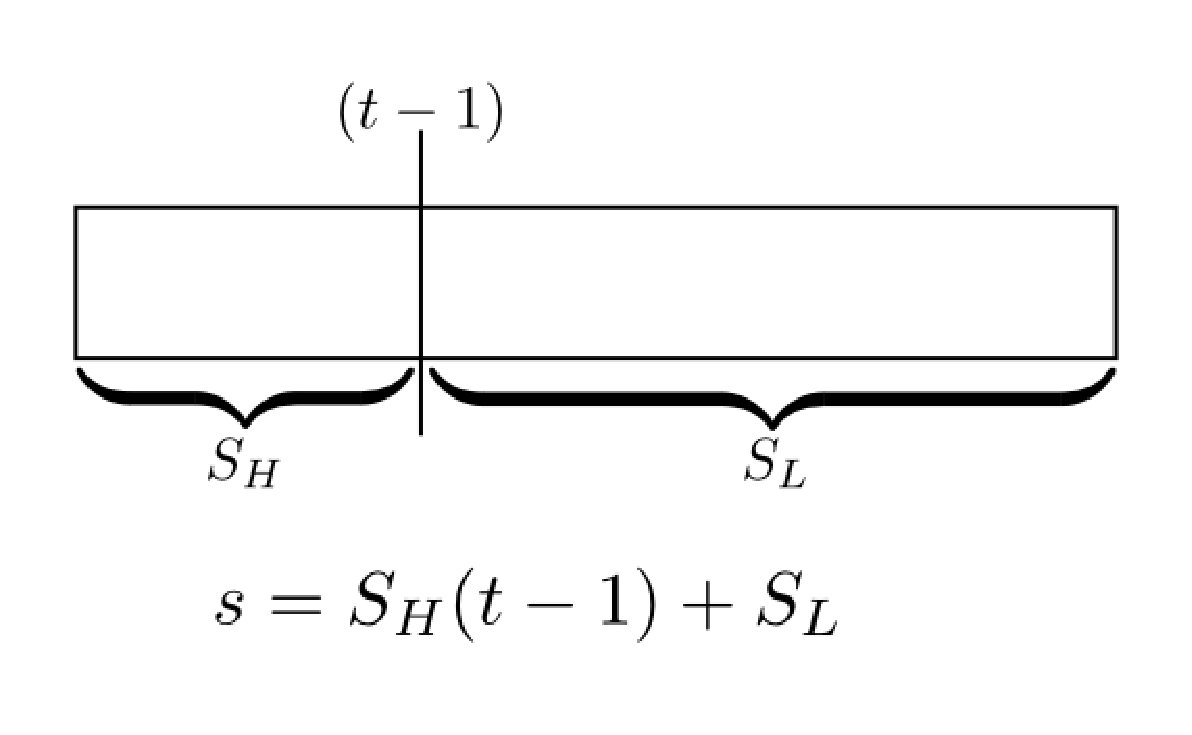
\includegraphics[width=2.5in]{t_adic.eps}
\caption{$(t-1)$ -adic representation of scalar $s$.}
\label{fig:t_adic}
\end{figure}

Figure \ref{fig:z_adicl} shows the final $z$-adic representation of scalar $s$. 
\begin{figure}[!ht]
\centering
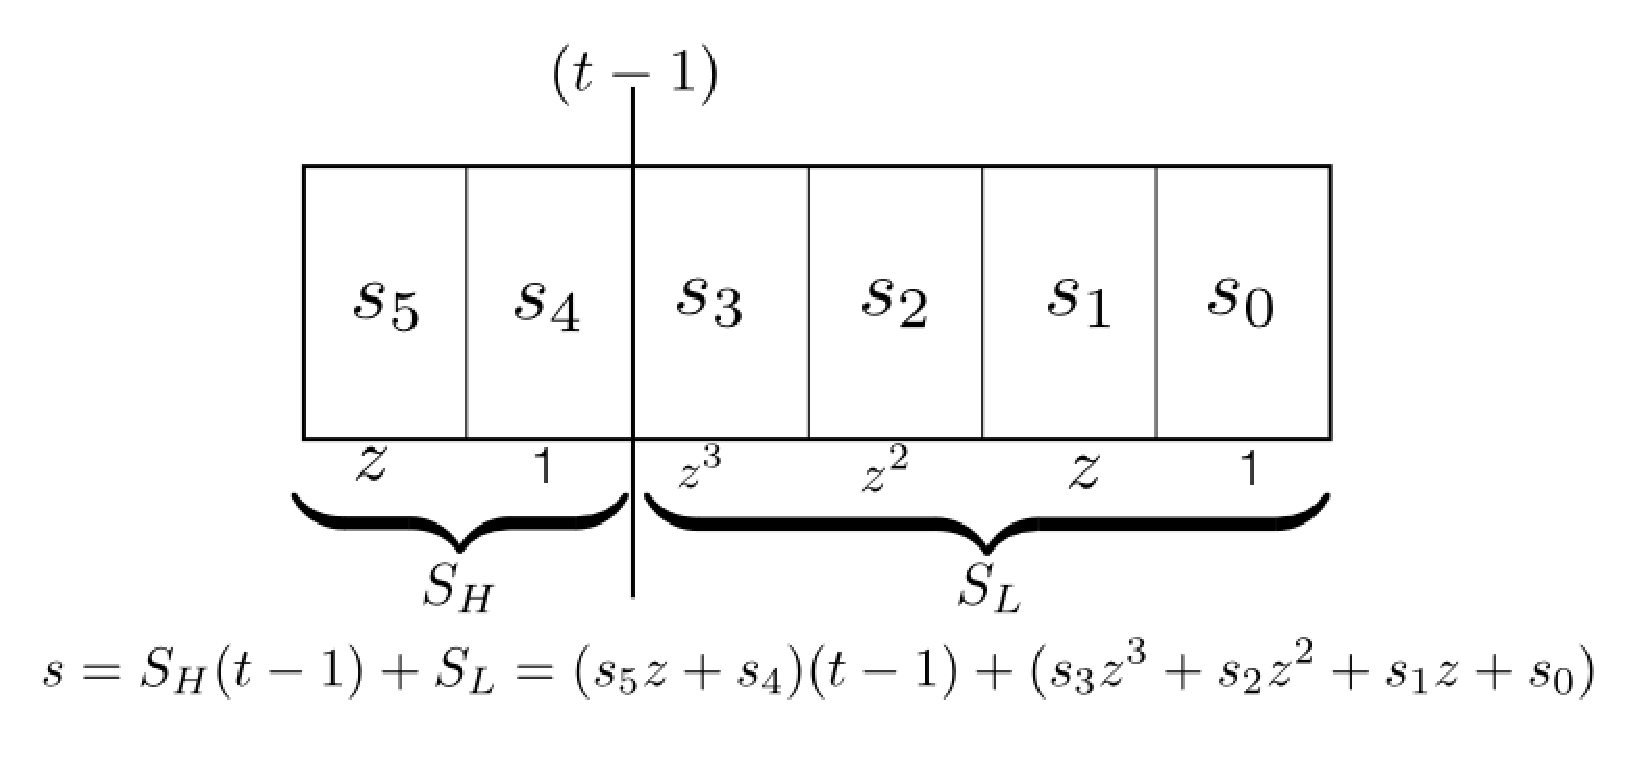
\includegraphics[width=2.5in]{z_adic.eps}
\caption{$z$-adic and $(t-1)$-adic representation of scalar $s$.}
\label{fig:z_adicl}
\end{figure}

Figure \ref{fig:z_sml} shows, an example of multi-scalar multiplication process, implemented in the experiment.
\begin{figure}[!ht]
\centering
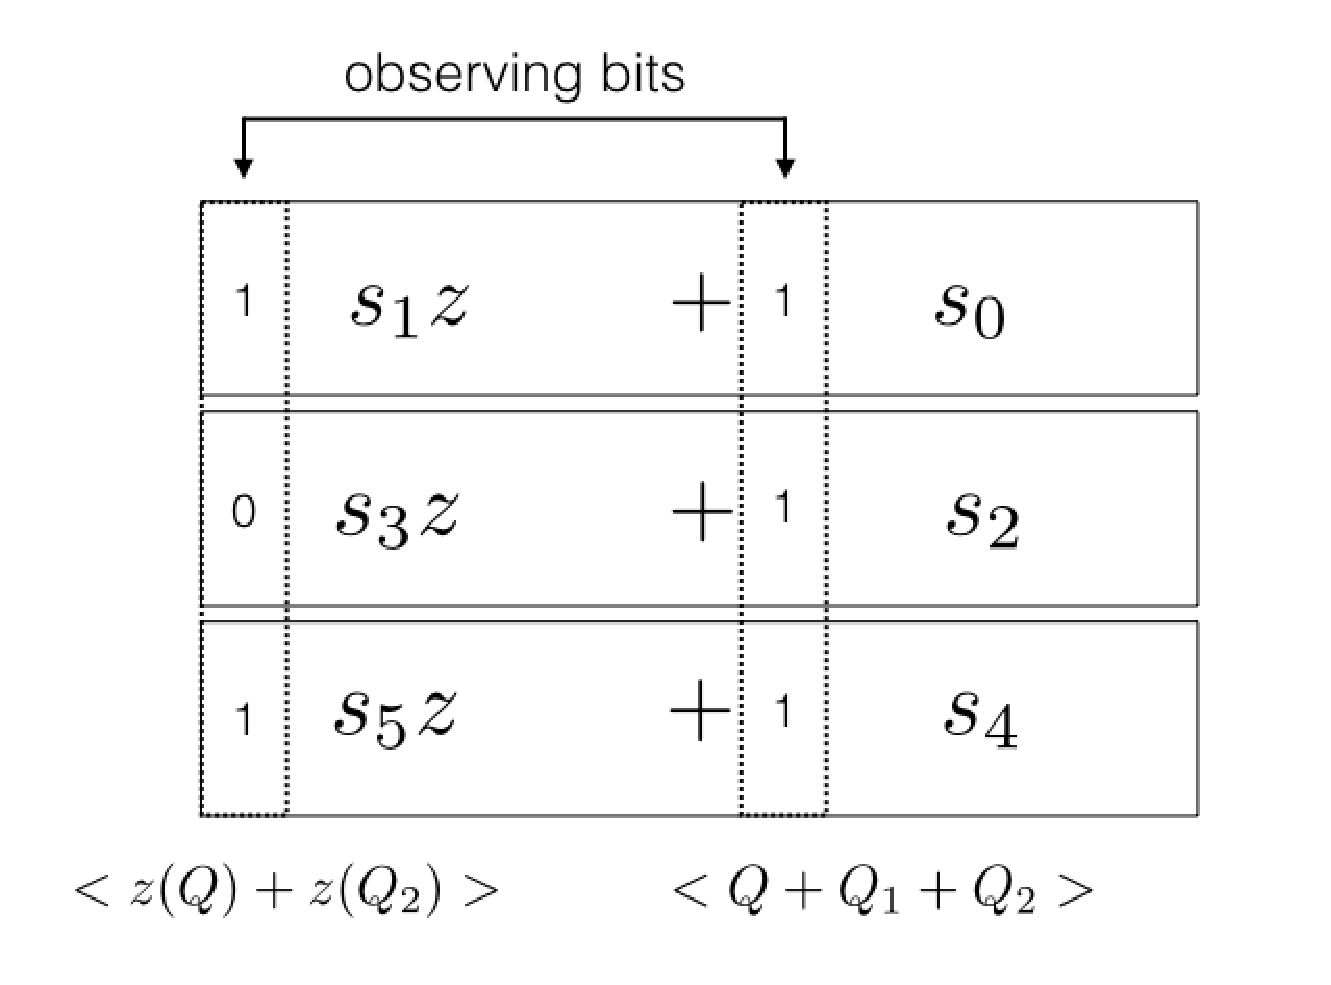
\includegraphics[width=2.5in]{z_sm.eps}
\caption{Multi-scalar multiplication of $s$ with Frobenius mapping.}
\label{fig:z_sml}
\end{figure}

\subsubsection{\g1, \g2 and \g3 groups.} In the context of pairing-based cryptography, especially on KSS curve, three groups $\g1, \g2$, and $\mathbb{G}_3$ are considered. From \cite{PAIRING:MANS13}, we define $\g1$, $\g2$ and $\g3$ as follows:
\begin{eqnarray}\label{eq:g1}
\g1 & = &  E(\F{p}{k}) [r] \cap \text{Ker}(\pi_p - [1]), \nonumber \\
\g2 & = &  E(\F{p}{k}) [r] \cap \text{Ker}(\pi_p - [p]), \nonumber \\
\g3 & = & \mF{p}{k}/(\mF{p}{k})^r, \nonumber
\end{eqnarray}
\begin{equation}
\alpha : \g1 \times \g2 \rightarrow \g3,
\end{equation}
where $\alpha$ denotes Ate pairing. In the case of KSS curve, $\g1, \g2$ are rational point groups and $\mathbb{G}_3$ is the multiplicative group in $\FQEN$. They have the same order $r$. 

Let us consider a rational point $Q\in \g2 \subset E(\F{p}{18})$.
In the case of KSS curve, it is known that $Q$ satisfies the following relations,
\begin{eqnarray}\label{eq:Q_rel1}
\big[p+1-t\big]Q & = & \cal O, \nonumber \\
\big[t-1\big]Q  & = & \big[p\big]Q.
\end{eqnarray}
\begin{eqnarray}\label{eq:Q_rel2}
[\pi_p -p]Q & = &\cal O, \nonumber \\
\pi_p(Q) & = & [p]Q.
\end{eqnarray}
Thus, these relations can accelerate a scalar multiplication in $\g2$.
Substituting $[p]Q$ in \eqref{eq:Q_rel1} we find $[t-1]Q = \pi_p(Q)$.

\subsubsection{$z$-adic representation of scalar $s$.}
From the previous work on optimal-ate pairing, Aranha et al. \cite{PAIRING:AFKMR12} derived the following relation from parameters \eqref{eq:kss_char}, \eqref{eq:kss_degree}, \eqref{eq:kss_trace} of KSS curve.
\begin{equation}\label{eq:aranha_relation}
z+3p-p^4 \equiv 0 \bmod {r}.
\end{equation}
Here $z$ is the mother parameter of KSS curve and $z$ is about six times smaller than the size of order $r$. 

Let us consider scalar multiplication $[s]Q$, where $0 \leq s < r$. From \eqref{eq:kss_degree} we know $r$ is the order of KSS curve  where $[r]Q=\cal O$. Here, the bit size of $s$ is nearly equal to $r$. In KSS curve $t$ is  $4/6$ times of  $r$. Therefore, let us first consider $(t-1)$-adic representation of $s$ as follows:
\begin{equation}\label{eq:t-1_adic}
s =  S_H(t-1)+S_L,
\end{equation}
where $s$ will be separated into two coefficients $S_H$ and $S_L$.  Size of $S_L$ will be nearly equal to the size of $(t-1)$ and $S_H$ will be about half of $(t-1)$. 
Now we consider $z$-adic representation of $S_H$ and $S_L$ as follows:
%Then SM  $[s]Q$ is calculated as follows:
\begin{eqnarray}\label{eq:scalar_mul_Q}
S_H & =  & s_5+ s_4,\nonumber \\
S_L & = & s_3 z^3+s_2 z^2+s_1 z+s_0.\nonumber 
\end{eqnarray}
Finally $s$ can be represented as 6 coefficients as follows:
\begin{eqnarray}\label{eq:sclar_final_rep}
s & =  & \sum_{i=0}^{3} s_iz^i + (s_4+s_5z)(t-1),\nonumber \\
s & = & (s_0+s_1z) + (s_2 +s_3z)z^2 +(s_4+s_5z)(t-1).
\end{eqnarray}

\subsubsection{Reducing the number of ECA and ECD for calculating $[s]Q$.}
Let us consider a scalar multiplication of $Q \in \g2$ in \eqref{eq:sclar_final_rep} as follows:
\begin{equation}\label{eq:proposed_scm_1}
[s]Q =  (s_0+s_1z)Q + (s_2 +s_3z)z^2Q +(s_4+s_5z)(t-1)Q.
\end{equation}
Let us denote $z^2Q$, $(t-1)Q$ of \eqref{eq:proposed_scm_1} as $Q_1$ and $Q_2$ respectively. From \eqref{eq:aranha_relation} and \eqref{eq:Q_rel2} we can derive the $Q_1$ as follows:
\begin{eqnarray}\label{eq:Q1}
Q_1& = & z^2 Q, \nonumber \\
& = & (9p^2-6p^5+p^8)Q,\nonumber \\
& = & 9\pi^2(Q)-6\pi^5(Q)+\pi^8(Q).
\end{eqnarray}
Using the properties of cyclotomic polynomial \eqref{eq:Q1} is simplified as,
\begin{eqnarray}\label{eq:Q1.1}
Q_1 & = & 8\pi^2(Q)-5\pi^5(Q),  \nonumber\\
& = & \pi^2(8Q)-\pi^5(5Q). 
\end{eqnarray}
And from the \eqref{eq:Q_rel1} and \eqref{eq:Q_rel2}, $Q_2$ is derived as,
\begin{equation}\label{eq:proposed_scm_2}
Q_2 = \pi (Q).
\end{equation}

Substituting \eqref{eq:Q1.1} and \eqref{eq:proposed_scm_2} in \eqref{eq:proposed_scm_1}, the following relation is obtained. 
\begin{equation}\label{eq:proposed_scm_0}
s[Q] =  (s_0+s_1z)Q + (s_2 +s_3z)Q_1 +(s_4+s_5z)Q_2.
\end{equation}
Using $z \equiv -3p + p^4$ (mod $r$) from \eqref{eq:aranha_relation}, $z(Q)$ can be pre-computed as follows:
\begin{equation}
z(Q) = \pi(-3Q) +\pi^4(Q).
\end{equation}
Table \ref{pre-compute} shows all the pre-computed values of rational points for the proposed method. In this paper pre-computed rational points are denoted such as $<Q+Q_2>$. Finally applying the the multi-scalar multiplication technique in \eqref{eq:proposed_scm_0} we can efficiently calculate the scalar multiplication. Figure \ref{fig:z_sml} shows an example of this multiplication. Suppose in an arbitrary index, from left to right, bit pattern of $s_1$, $s_3$, $s_5$ is 101 and at the same index $s_0$, $s_2$, $s_4$ is 111. Therefore we apply the pre-computed points $< z(Q)+z(Q_2) >$ and $<Q+Q_1+Q_2>$ as ECA in parallel. Then we perform ECD and move to the right next bit index to repeat the process until maximum length $z$-adic coefficient becomes zero.

\renewcommand{\baselinestretch}{1.5}
\begin{table}[!ht]
\centering
\caption{ Pre-computed values of rational point for efficient scalar multiplication}
\label{pre-compute}
\begin{tabular}{|c|c|}
\hline 
• & $z(Q)$ \\ 
\hline 
$Q_1$ & $z(Q_1)$  \\ 
\hline 
$Q_2$ & $z(Q_2)$ \\ 
\hline 
$Q_1+Q_2$ & \quad  $ z(Q_1)+ z(Q_2) $ \quad \\ 
\hline 
$Q+Q_2$ & $ z(Q)+ z(Q_2) $ \\ 
\hline 
$Q+Q_1$ & $  z(Q)+ z(Q_1) $ \\ 
\hline 
 \quad $Q+Q_1+Q_2$ \quad  \quad &   \quad  $ z(Q)+ z(Q_1)+ z(Q_2)$  \quad \\ 
\hline 
\end{tabular} 
\end{table}
\renewcommand{\baselinestretch}{1.0}
As shown in Figure \ref{fig:z_sml}, during scalar multiplication in parallel, we are considering \eqref{eq:sclar_final_rep} like 3 pair of coefficients of $z$-adic representation. If we consider 6-coefficients for parallelization, we will need to calculate $2^6 \times 2$ pre-computed points. The chance of appearing each pre-computed point in parallel calculation will be only once which will make the pre-calculated points redundant.  

\section{Experimental result evaluation}
In order to demonstrate the efficiency of the proposal, this section shows some experimental result with the calculation cost. In the experiment we have compared the proposed method with three well studied method of scalar multiplication named binary method, sliding-window method and non-adjacent form (NAF) method.

In the experiment the following parameters are considered for the KSS curve $y^2 = x^3 + 11$. 
\begin{eqnarray}
z & = & 65   \mbox{-bit},  \nonumber \\ 
p  & = & 511 \mbox{-bit},  \nonumber \\ 
r  & = & 378 \mbox{-bit} ,\nonumber \\ 
t  & = & 255  \mbox{-bit}. \nonumber
\end{eqnarray}
The mother parameter $z$ is also selected accordingly to find out $\g2$ rational point $Q$. 

500 scalar numbers of size (about 377-bit) less than order $r$ is generated randomly in the experiment. Then average number of ECA and ECD for the proposed method and the three other methods is calculated for a scalar multiplication. 13  pre-computed ECA is taken into account while the average is calculated for the proposed method. In case of sliding-window method window size 4-bit is considered. Therefore 14 pre-computed ECA is required. In addition, average execution time of the proposed method and the three other methods is also compared.

Table \ref{tab1} shows the environment, used to experiment and evaluate the proposed method.  
\renewcommand{\baselinestretch}{1.5}
\begin{table}[!ht]
\renewcommand{\arraystretch}{1.3}
\centering
\caption{ Computational Environment}
\label{tab1}
\begin{tabular}{|c|c|c|}
\hline 
• & PC & iPhone6s \\ 
\hline \hline 
CPU {\textsuperscript{*}} & \quad 2.7 GHz Intel Core i5 \quad & \quad Apple A9 Dual-core 1.84 GHz \quad \\ 
\hline 
Memory & 16 GB & 2 GB \\ 
\hline 
OS & Mac OS X 10.11.4 &  iOS 9.3.1 \\ 
\hline 
Compiler & gcc 4.2.1 & gcc 4.2.1 \\ 
\hline 
\quad Programming Language \quad  & C & Objective-C, C \\ 
\hline 
Library & GNU MP 6.1.0 & GNU MP 6.1.0 \\ 
\hline 
\midrule[.5pt]
\multicolumn{3}{l}{\textsuperscript{*}\footnotesize{Only single core is used from two cores.}}\\
\end{tabular} 
\end{table}
\renewcommand{\baselinestretch}{1.0}

\renewcommand{\baselinestretch}{1.5}
\begin{table}[!ht]
%\renewcommand{\arraystretch}{1.3}
\centering
\caption{ Comparative result of average number of ECA and ECD and execution time in [ms] for scalar multiplication}
\label{tab_opeation}
\begin{tabular}{|c|c|c|c|c|c|c|}
\hline
 & \multicolumn{6}{|c|}{\quad Average ECA, ECD and  execution time [ms] comparison \quad} \\ \hline
& \multicolumn{2}{|c|}{PC} & PC & \multicolumn{3}{|c|}{iPhone 6s}  \\ 
 \hline \hline
Methods & \quad \#ECA \quad & \quad \#ECD \quad & \quad Execution time \quad & \multicolumn{3}{|c|}{\quad Execution time}\\ 
 \hline
Binary  & 187 & 376 &  $1.15 \times 10^3$  &  \multicolumn{3}{|c|} { $1.3 \times 10^3$}\\ \hline
\quad Sliding-window \quad & 103 & 376 &  $1.14 \times 10^3$  &  \multicolumn{3}{|c|} { $1.10 \times 10^3$}\\ \hline
 NAF  & 126 & 377 &  $1.03 \times 10^3$  &  \multicolumn{3}{|c|} { $1.13 \times 10^3$}\\ \hline
 \quad Proposed  \quad \quad & 124 & 64 & $3.36 \times 10^2$  &   \multicolumn{3}{|c|}{$3.76 \times 10^2$}\\ \hline
\end{tabular} 
\end{table}
\renewcommand{\baselinestretch}{1.0}
Analyzing  Table \ref{tab_opeation} we can find that our proposed method requires more than 5 times less ECD than binary method, sliding-window method and NAF method. The number of ECA is also reduced in the proposed method by about 30\% than binary method.  

In this experiment, execution time may seems slower than other efficient algorithm such as Montgomery reduction. 
But the main purpose of this execution time comparison is to compare the ratio of the execution time of the proposed method with other well studied methods. The result shows that proposed method is at least 3 times faster than the other methods. Other acceleration techniques such as Montgomery reduction, Montgomery trick and efficient coordinates can be applied to this proposed method to enhance its execution time.

\section{Conclusion and future work}
In this paper we have proposed an efficient method to calculate elliptic curve scalar multiplication using Frobenious mapping  over KSS curve in context of pairing based cryptography. We have also applied $(t-1)$-adic and $z$-adic representation on the scalar and have applied multi-scalar multiplication technique to  calculate scalar multiplication in parallel. We have evaluated and analyzed the improvement by implementing a simulation for large size of scalar in 192-bit security level. The experimented result shows that our proposed method is at least 3 times efficient in context of execution time and takes 5 times less number of elliptic curve doubling than binary method, sliding-window method and non-adjacent form method. As a future work we would like to enhance its computation time by applying not only Montgomery reduction but also skew Frobenius  map in  sub-field isomorphic rational point group technique and test the effect of the improvement in some pairing application for practical case. 

\section*{Acknowledgment}
This work was partially supported by the Strategic Information and Communications R\&D Promotion Programme (SCOPE) of Ministry of Internal Affairs and Communications, Japan. 

%\medskip
%\bibliographystyle{1}
%\bibliography{wisa_ref.bib}

% \end{document} 
\chapter{IEICE 2016} 
\chapter{Improved \texorpdfstring{$\g{2}$}{G2} Scalar Multiplication over KSS-18 Curve} 
\label{Chapter_IEICE}
\section{Introduction}
\subsection{Background and Motivation}
Recall that, pairing-based cryptography has attracted many researchers since Sakai et al. \cite{EPRINT:SakKas03} and Joux et al. \cite{JC:Joux04} independently proposed a cryptosystem based on elliptic curve pairing. This has encouraged to invent several innovative pairing-based cryptographic applications such as broadcast encryption \cite{C:BonGenWat05} and group signature authentication \cite{C:BonBoySha04}, that has increased the popularity of pairing-based cryptographic research.

However, using pairing-based cryptosystems in the industrial state is still restricted by its expensive operational cost concerning time and computational resources in a practical case. 
In order to make it practical, several pairing techniques such as Ate \cite{DBLP:reference/crc/2005ehcc}, Optimal-Ate \cite{DBLP:journals/tit/Vercauteren10}, twisted Ate \cite{EPRINT:MKHO07}, $\chi$-Ate \cite{PAIRING:NASKM08} and \textit{subfield twisted} Ate \cite{PAIRING:DevScoDah07} pairings have gained much attention since they have achieved quite efficient pairing calculation in certain pairing friendly curve. 
Researchers continue to find an efficient way to implement pairing to make it practical enough for industrial standardization. 

In such consequences, this chapter focuses on a peripheral technique of Ate-based pairings that is scalar multiplication defined over Kachisa-Schaefer-Scott (KSS) curve \cite{EPRINT:KacSchSco07} of embedding degree 18. 
Scalar multiplication over higher degree rational point groups is often regarded as the bottleneck for faster pairing-based cryptography.

As aforementioned, pairing is a bilinear map of two rational point groups $\g1$ and $\g2$ to a multiplicative group $\g3$ \cite{Silverman}.
The typical notation of pairing is $\g1 \times \g2 \rightarrow \g3$.
In  Ate-based pairing, $\g1$, $\g2$ and $\g3$ are defined as:
\begin{eqnarray}\label{eqn_g1g2g3_group_kss18}
\g1 & = &  E(\F{p}{k}) [r] \cap \text{Ker}(\pi_p - [1]), \nonumber \\
\g2 & = &  E(\F{p}{k}) [r] \cap \text{Ker}(\pi_p - [p]), \nonumber \\
\g3 & = & \mF{p}{k}/(\mF{p}{k})^r, \nonumber
\end{eqnarray}
\begin{equation}
\alpha : \g1 \times \g2 \rightarrow \g3,  \nonumber
\end{equation}
where $\alpha$ denotes Ate pairing.
Pairings are often defined over specific extension field $\FQK$, where $p$ is the prime number, also known as characteristics, and $k$  is the minimum extension degree for pairing also called \textit{embedding} degree. 
The set of rational points $E(\FQK)$ are defined over a specific pairing-friendly curve of an embedded extension field of degree $k$.
This chapter has considered Kachisa-Schaefer-Scott (KSS) \cite{EPRINT:KacSchSco07} pairing friendly curves of emebdding degree $k=18$ described in \cite{EPRINT:FreScoTes06}.


\subsection{Contribution}
Scalar multiplication is often considered to be one of the most time-consuming operations in the cryptographic scene. 
Efficient scalar multiplication is one of the critical factors for making the pairing practical over KSS-18 curve.

This chapter focuses on efficiently performing scalar multiplication on rational points defined over rational point group $\g2$ by scalar $s$ since scalar multiplication is required repeatedly in the cryptographic calculation.
However, in asymmetric pairing such as Ate-based pairing, scalar multiplication of $\g2$ rational points is essential as no mapping function is explicitly given between $\g1$ to $\g2$.
By the way, as shown in the definition, $\g1$ is a set of rational points defined over the prime field, and there are several pieces of research \cite{CANS:SNOKM08} for efficient scalar multiplication in $\g1$.

The typical approach to accelerate scalar multiplication are log-step algorithm such as binary and non-adjacent form (NAF) methods, but the more efficient approach is to use Frobenius mapping in the case of $\g2$ that is defined over $\F{p}{k}$.
Moreover when a sextic twist of the pairing-friendly curve exists, then we apply skew Frobenius map on the isomorphic sextic-twisted subfield rational points. Such a technique will reduce the computational cost to a great extent.

In this chapter, we have exploited the sextic twisted property of KSS-18 curve and utilized skew Frobenius map to reduce the computational time of scalar multiplication on $\g2$ rational point. 
Utilizing the relation $z \equiv -3p + p^4 \bmod {r}$,\footnote{$z$ is the mother parameter of KSS-18 curve, and $z$ is about six times smaller than the size of order $r$.} derived by Aranha et al.,\cite{PAIRING:AFKMR12} and the properties of $\g2$ rational point, the scalar can be expressed as $z$-adic representation.
Together with skew Frobenius mapping and $z$-adic representation the scalar multiplication can be further accelerated.  
We have utilized this relation to construct $z$-adic representation of scalar $s$ which is introduced in \secref{section_zadic_chapter_g2scm_kss18}. 
Besides with Frobenius mapping and $z$-adic representation of $s$, we applied the multi-scalar multiplication technique to compute elliptic curve addition in parallel in the proposed scalar multiplication.
We have compared our proposed method with three other well-studied methods named binary method, sliding-window method, and non-adjacent form method. 
The comparison shows that our proposed method is about 60 times faster than the plain implementations of methods as mentioned above in execution time. The comparison also reveals that the proposed method requires more than five times less elliptic curve doubling than any of the compared methods.

\subsection{Related Works} 
There are several works \cite{DBLP:journals/ieicet/NogamiSONAM09}\cite{CANS:SNOKM08} on efficiently computing scalar multiplication defined over Barreto-Naehrig\cite{SAC:BarNae05} curve along with efficient extension field arithmetic \cite{C:BaiPaa98}. 
This chapter focuses on scalar multiplication on KSS-18 curve.


\section{Preliminaries}
In this section, we recall some already introduced preliminaries for a comprehensible understanding of the proposal. 
We will briefly review the elliptic curve scalar multiplication. 
Throughout this chapter, $p$ and $k$ denote characteristic and embedding extension degree, respectively. $\FQK$ denotes $k$-the extension field over prime field $\Fp$ and $\mF{p}{k}$ denotes the multiplicative group in $\FQK$.

\subsection{Elliptic Curve}
An elliptic curve \cite{washington2003elliptic} defined over $\Fp$ is generally represented by \textit{affine coordinates} \cite{Silverman} as follows;
%Let $\Fp$ be a prime field. Elliptic curve over $\Fp$ is defined as,
\begin{equation}\label{eqn_ellipticcurve_chapter_g2scm_kss18}
E/\Fp : y^2=x^3+ax+b,
\end{equation}
where $ 4a^3+27b^2 \neq 0$ and $a,b \in \Fp$. A pair of coordinates $x$ and $y$ that satisfy \eqref{eqn_ellipticcurve_chapter_g2scm_kss18} are known as \textit{rational points} on the curve. 
We refer to \secref{sec:chap:fund:ecc} of \chref{chap:fundamentals} for the elliptic curve point operation (ECA, ECD) and the scalar multiplication algorithms.


\subsection{KSS Curve of Embedding Degree \texorpdfstring{$k=18$}{\textit{k=18}}}
We recall \secref{sec:ch:icisc:kss18curve} from \chref{ch:optate_kss18_icisc2016} for the definition of KSS-18 curve for comprehensive understanding of the chapter.
Here we change the mother parameter notation as $z$.
%In  \cite{EPRINT:KacSchSco07}, Kachisa, Schaefer, and Scott proposed a family of non super-singular Brezing-Weng pairing-friendly elliptic curves using elements in the cyclotomic field. 
In what follows this chapter considers the KSS curve of embedding degree $k=18$ since it holds \textit{sextic twist}. 
The equation of KSS curve defined over $\FQEN$ is given as follows:
\begin{equation}\label{eqn_kss18curve_chapter_g2scm_kss18}
E:Y^2=X^3+b, \quad \mbox{($b \in \Fp$)},
\end{equation}
where $b \neq 0$ and $X,Y \in \FQEN$. Its characteristic $p$, Frobenius trace $t$ and order $r$ are given systematically by using an integer variable $z$ as follows:
\begin{subequations}
	\begin{eqnarray}
	p(z) &= & (z^8 +5z^7 +7z^6 +37z^5 +188z^4 +259z^3  \nonumber \\
	& & + 343z^2 +1763z+2401)/21,\\\label{eq:kss_char_chapter_g2scm_kss18}
	r(z) &= &(z^6 + 37z^3 + 343)/343,\label{eq:kss_degree_chapter_g2scm_kss18}  \\
	t(z) &=& (z^4 + 16z + 7)/7, \label{eq:kss_trace_chapter_g2scm_kss18} 
	\end{eqnarray}
\end{subequations} 
where $z$ is such that $z \equiv 14$ (mod $42$) and the $\rho$ value is $\rho = (\log_2 p/\log_2 r) \approx 1.33$.

In some previous work of  Aranha et al. \cite{PAIRING:AFKMR12} and Scott et al. \cite{IMA:Scott11} has mentioned that the size of the characteristics $p$ to be 508 to 511-bit with order $r$ of 384-bit  for 192-bit security level.  
Therefore this chapter used parameter settings according to the suggestion of \cite{PAIRING:AFKMR12} for 192-bit security on KSS-18 curve in the simulation implementation. In recent work, Kim et al. \cite{C:KimBar16} has suggested updating the key sizes in pairing-based cryptography due to the development of a new discrete logarithm problem over the finite field. The parameter settings used in this chapter does not completely end up at the 192-bit security level according to \cite{C:KimBar16}. However, the parameter settings used in this chapter shows the resemblance of the proposal with the experimental result.

\subsection{\texorpdfstring{$\FQEN$}{Fp18} Extension Field Arithmetic}
Pairing-based cryptography requires to perform an arithmetic operation in extension fields of degree $k \geq 6$\cite{Silverman}. 
We recall \secref{sec:ch:icisc:towering_optate_KSS18} of \chref{ch:optate_kss18_icisc2016} for $\FQEN$ construction.

Let $(p-1)$ is divisible by 3 and $c$ is a quadratic and cubic non residue in $\Fp$. In KSS curve \cite{EPRINT:KacSchSco07}, where $k=18$, $\FQEN$ is constructed  with irreducible binomials by the following towering scheme.
\begin{equation}
\begin{cases}
\F{p}{3} = \F{p}{}[i]/(i^3-c),  \text{where $c = 2$ is the best choice,}\nonumber \\ 
\F{p}{6} = \F{p}{3}[v]/(v^2-i), \nonumber \\ 
\F{p}{18} = \F{p}{6}[\theta]/(\theta^3-v). \nonumber \\ 
\end{cases}
\end{equation}\label{eq:KSS18_towering_chapter_g2scm_kss18}
where the base extension field is $\FQTH$ for the \textit{sextic twist} of KSS-18 curve.

\subsection{Frobenius Mapping of Rational Points in  \texorpdfstring{ $E(\FQEN)$}{E(Fp18)}} \index{KSS-18: Frobenius map}
Let $(x,y)$ be certain rational point in $E(\FQEN)$. 
Frobenius map $\pi_p : (x,y) \mapsto  (x^p,y^p)$ is the $p$-th power of the rational point defined over $\FQEN$. 
Sakemi et al. \cite{CANS:SNOKM08} showed an efficient scalar multiplication by applying skew Frobenius mapping in the context of Ate-based pairing in BN curve of embedding degree $k=12$.  In this chapter, we have utilized the skew Frobenius mapping technique for efficient scalar multiplication for the KSS-18 curve.

\subsection{Sextic Twist of KSS-18 Curve}  \index{KSS-18: Sextic twist}
We recall \secref{sec:ch:icisc:sextictwist_KSS18} from \chref{ch:optate_kss18_icisc2016} for the definition of sextic twist of KSS-18 curve.
Let the embedding degree $k = 6e$, where $e$ is positive integer, \textit{sextic} twist is given as follows:
\begin{eqnarray}
E:  \quad y^2 & = & x^3+b, \quad b \in \Fp, \\
E'_6: \quad y^2 & =  & x^3+bu^{-1},
\end{eqnarray}  
where $u$ is a quadratic and cubic non residue in $E(\F{p}{e})$ and $3|(p^e-1)$.  Isomorphism between $E'_6(\F{p}{e})$ and $E(\F{p}{6e})$, is given as follows:
\begin{eqnarray}
\psi_6 : \begin{cases}
E'_6(\F{p}{e}) \rightarrow E(\F{p}{6e}),\\
(x,y) \quad \mapsto (xu^{1/2},yu^{1/2}).
\end{cases}
\end{eqnarray}
In context of Ate-based pairing for KSS curve of embedding degree 18, sextic twist is considered to be the most efficient.

\section{Improved Scalar Multiplication for \texorpdfstring{$\g2$}{G2}}
This section will introduce the proposal for efficient scalar multiplication of $\g2$ rational points defined over KSS curve of embedding degree $k=18$ in context of Ate-based pairing. 
An overview the proposed method is given next before diving into the detailed procedure.
\subsection{Overview of the Proposal} 
Figure \ref{fig:_overallprocess_towering_chapter_g2scm_kss18} shows an overview of overall process of proposed scalar multiplication.
\begin{figure*}[ht]
	\centering
	%\resizebox{0.7\columnwidth}{!}{
	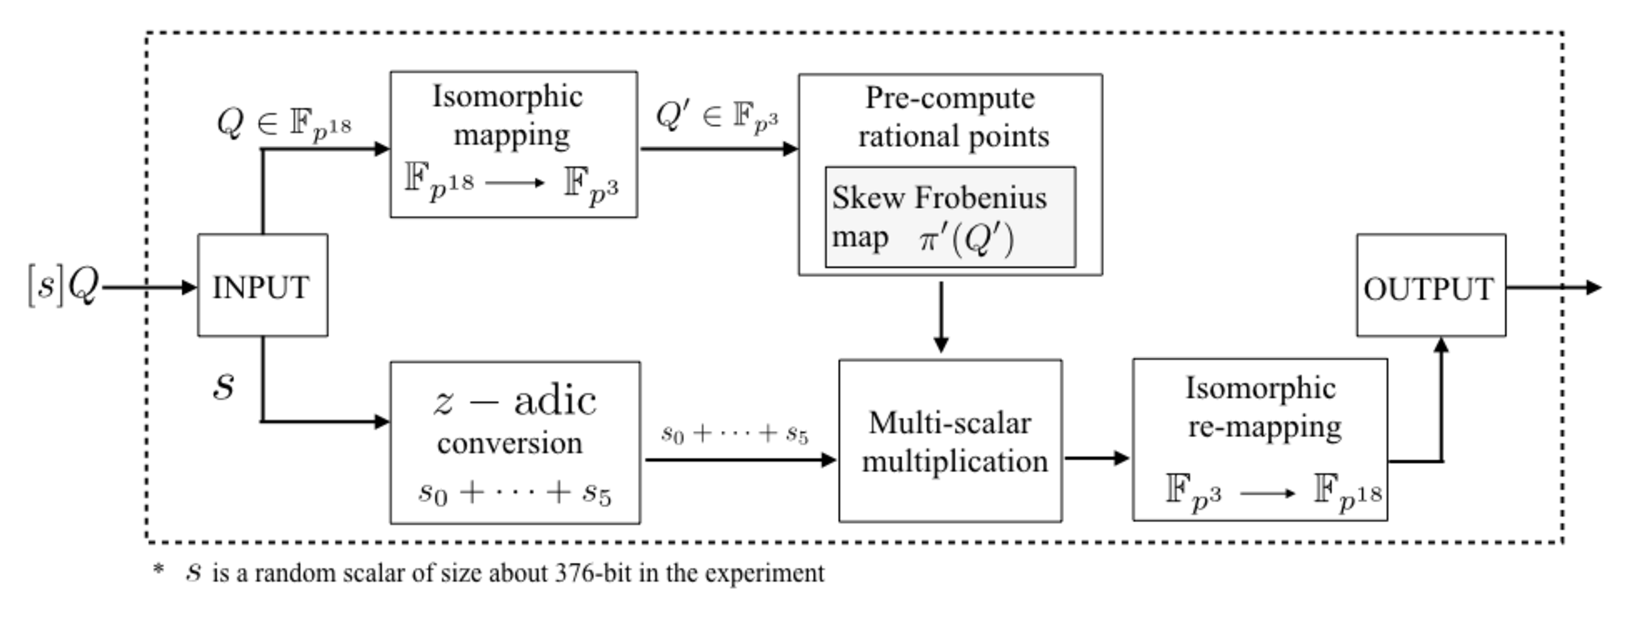
\includegraphics[width=\linewidth, keepaspectratio]{process.eps}
	%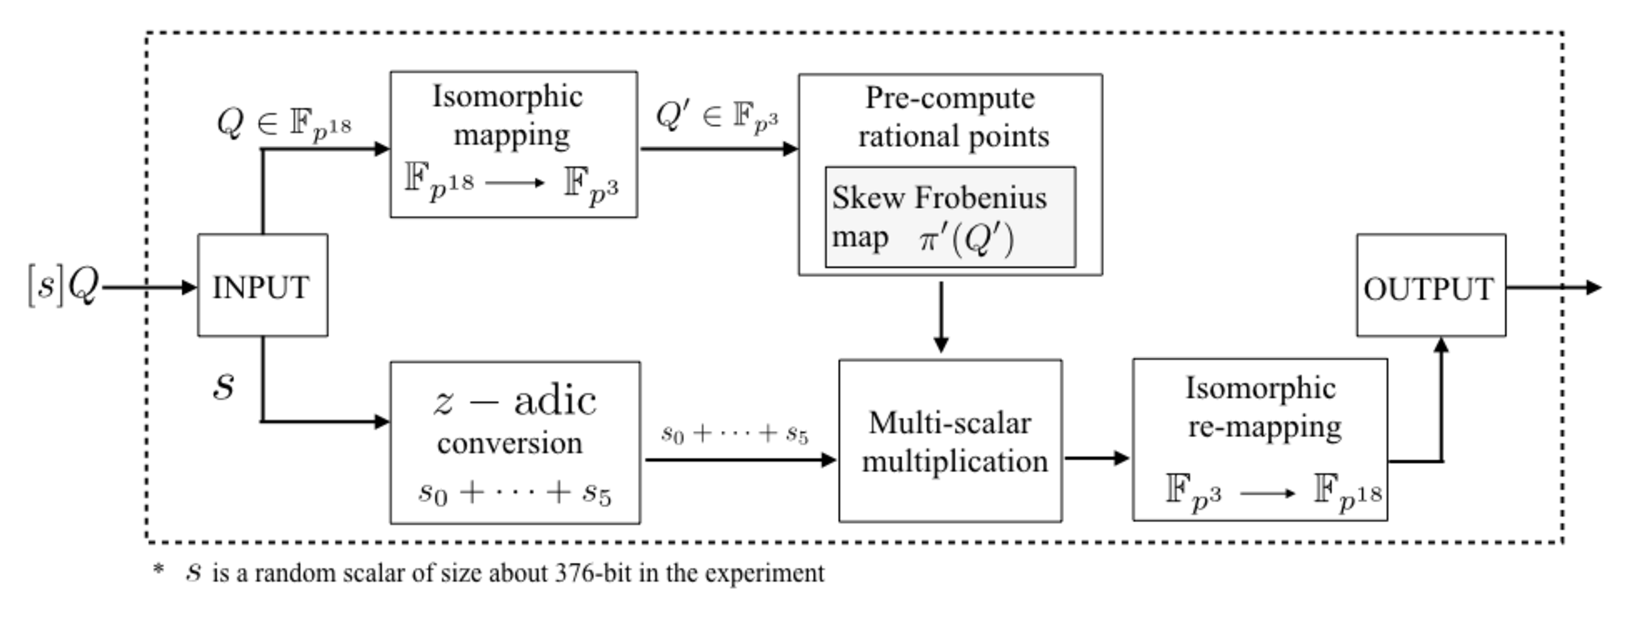
\includegraphics[width=6.5in]{process.eps}
	\caption{Overview of the proposed scalar multiplication for KSS-18 curve.}
	\label{fig:_overallprocess_towering_chapter_g2scm_kss18}
\end{figure*}
Rational point groups $\g1$, $\g2$ and multiplicative group $\g3$ groups will be defined at the beginning. Then a rational point $Q\in \g2 \subset E(\F{p}{18})$ will be calculated.
$Q$ has a  special vector representation with 18 $\Fp$ elements for each coordinates. 
A random scalar $s$ will be considered for scalar multiplication of $[s]Q$ which is denoted as input in  Figure \ref{fig:_overallprocess_towering_chapter_g2scm_kss18}. After that we will consider an isomorphic map of rational point $Q\in \g2 \subset E(\F{p}{18})$ to its sextic twisted rational point $Q' \in \g2' \subset E'(\F{p}{3})$. At the same time, we will obtain the $z$-adic representation of the scalar $s$. Next, some rational points defined over $E'(\FQTH)$ will be pre-computed by applying the skew Frobenius mapping. After that, a multi-scalar multiplication technique will be applied to calculate the scalar multiplication in parallel. The result of this scalar multiplication will be defined over $\FQTH$. Finally, the result of the multi-scalar multiplication will be re-mapped to a rational point in $E(\FQEN)$ to get the final result.

\subsection{\g1, \g2 and \g3 Groups} 
In the context of pairing-based cryptography, especially on KSS-18 curve, three groups $\g1, \g2$, and $\mathbb{G}_3$ are considered. From \cite{PAIRING:MANS13}, we define $\g1$, $\g2$ and $\g3$ as follows:
\begin{eqnarray}\label{eq:g1_chapter_g2scm_kss18}
\g1 & = &  E(\F{p}{18}) [r] \cap \text{Ker}(\pi_p - [1]), \nonumber \\
\g2 & = &  E(\F{p}{18}) [r] \cap \text{Ker}(\pi_p - [p]), \nonumber \\
\g3 & = & \mF{p}{18}/(\mF{p}{18})^r, \nonumber
\end{eqnarray}
\begin{equation}
\alpha : \g1 \times \g2 \rightarrow \g3,
\end{equation}
where $\alpha$ denotes Ate pairing. In the case of KSS-18 curve, $\g1, \g2$ are rational point groups and $\mathbb{G}_3$ is the multiplicative group in $\FQEN$. They have the same order $r$. 

In context of KSS-18 curve, let us consider a rational point $Q\in \g2 \subset E(\F{p}{18})$ where $Q$ satisfies the following relations,
\begin{eqnarray}\label{eq:Q_rel1_chapter_g2scm_kss18}
\big[p+1-t\big]Q & = & \cal O, \nonumber \\
\big[t-1\big]Q  & = & \big[p\big]Q.
\end{eqnarray}
\begin{eqnarray}\label{eq:Q_rel2_chapter_g2scm_kss18}
[\pi_p -p]Q & = &\cal O, \nonumber \\
\pi_p(Q) & = & [p]Q.
\end{eqnarray}
where  $[t-1]Q = \pi_p(Q)$, by substituting $[p]Q$ in \eqref{eq:Q_rel1_chapter_g2scm_kss18}.


\subsection{Isomorphic Mapping between \texorpdfstring{$Q$}{Q} and  \texorpdfstring{$Q'$}{Q'}}
\label{sec:ch:ieice2016:mappingQtoQprime}
Let us consider $E$ is the KSS-18 curve in base field $\FQTH$  and $E'$ is sextic twist of $E$ given as follows: 
\begin{eqnarray}
E:y^2 & = &x^3+b,\\
E':y^2 & = & x^3+bi, \label{eq:KSS18_Twist_chapter_g2scm_kss18}
\end{eqnarray}
where $b \in \Fp$; $x, y, i \in \FQTH$ and basis element $i$ is the quadratic and cubic non residue in $\FQTH$.

Rational point $Q\in \g2 \subset E(\F{p}{18})$ has a  special vector representation with 18 $\Fp$ elements for each $x_Q$ and $y_Q$ coordinates.
Figure \ref{fig:Q_structure_chapter_g2scm_kss18} shows the structure of the coefficients of $Q \in \FQEN$ and its sextic twisted isomorphic rational point $Q' \in \FQTH$ in KSS-18 curve.
\begin{figure}[ht]
	\centering
	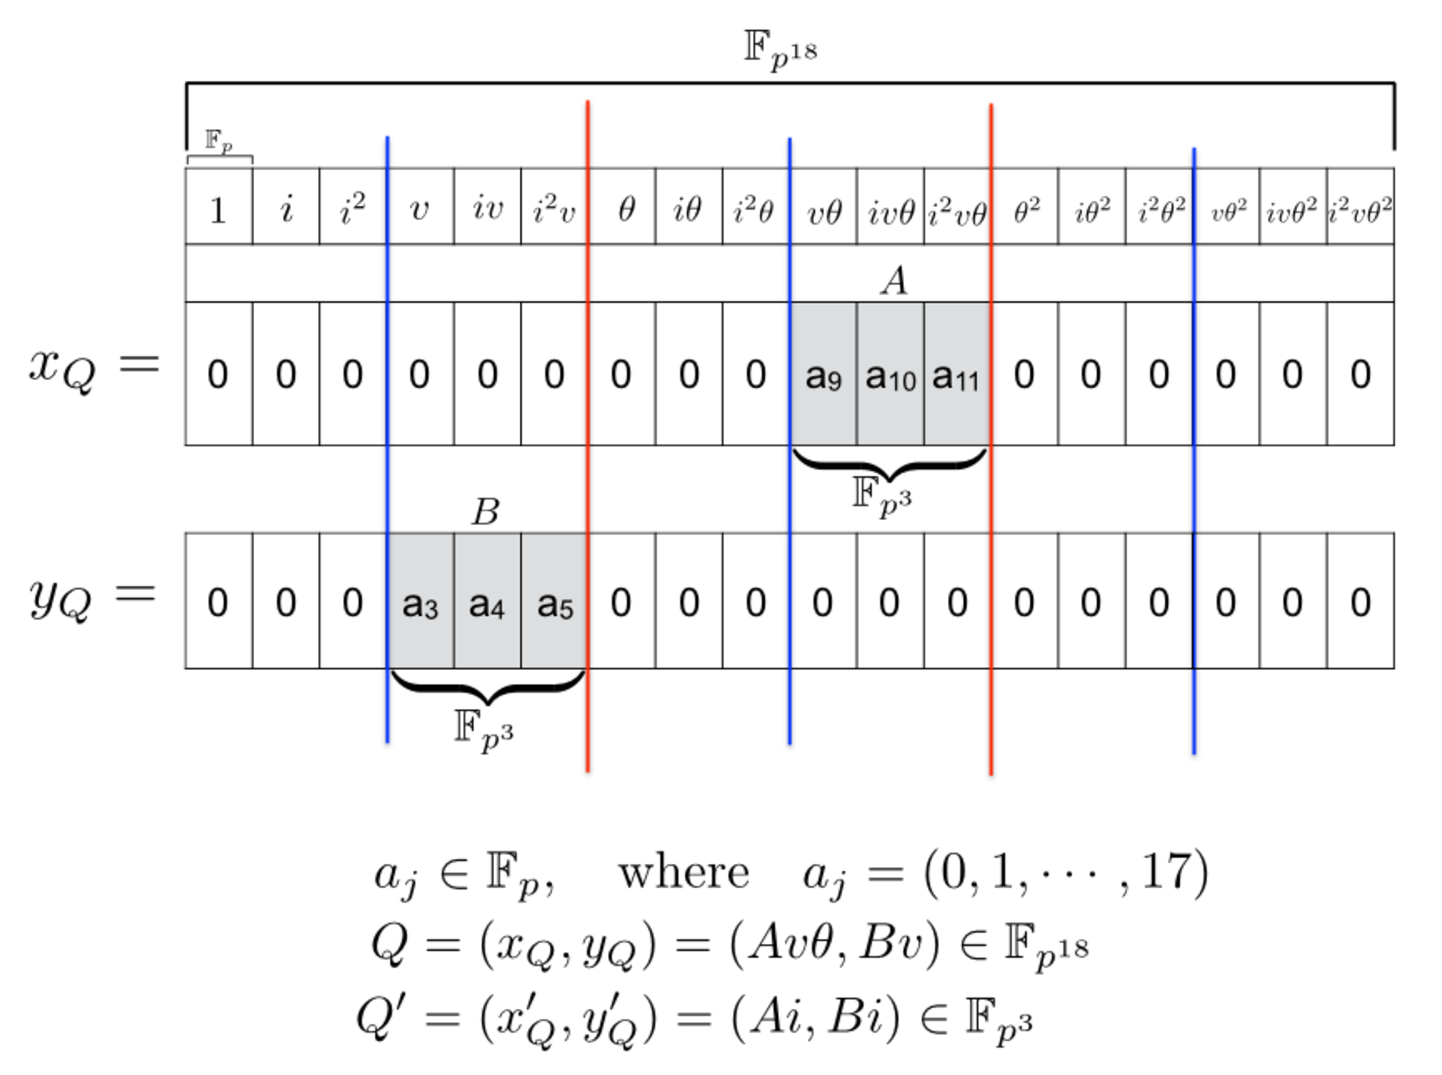
\includegraphics[width=\linewidth, keepaspectratio]{structure.eps}
	\caption{ $Q \in \FQEN$ and its sextic twisted isomorphic rational point $Q' \in \FQTH$ structure in KSS-18 curve.}
	\label{fig:Q_structure_chapter_g2scm_kss18}
\end{figure}
Among 18 elements, there are 3 continuous nonzero $\Fp$ elements which belongs to a $\FQTH$ element. The other coefficients are zero.
In this chapter, considering parameter settings given in Table \ref{table:parameters_chapter_g2scm_kss18} of section 4; $Q$ is given as $Q = (Av\theta, Bv)$,  showed in Figure \ref{fig:Q_structure_chapter_g2scm_kss18}, where $A, B \in \FQTH$ and $v$ and $\theta$ are the basis elements of $\F{p}{6}$ and $\FQEN$ respectively. 

Let us consider the sextic twisted isomorphic subfield rational point of $Q$ as $Q' \in \g2' \subset E'(\F{p}{3})$ and $x'$ and $y'$ as the coordinates of $Q'$.

\subsubsection{Mapping \texorpdfstring{$Q = (Av\theta, Bv)$}{}  to the Rational Point  \texorpdfstring{$Q' = (x',y')$}{}}

Let's multiply  $\theta^{-6}$ with both side of \eqref{eq:KSS18_Twist_chapter_g2scm_kss18}, where $i=\theta^6$ and $v = \theta^3$.
\begin{equation}\label{eq:sextic_div_theta_chapter_g2scm_kss18}
E':  \Big(\frac{y}{\theta^3}\Big)^2  = \Big(\frac{x}{\theta^2}\Big)^3+ b.
\end{equation}
Now $\theta^{-2}$ and $\theta^{-3}$ of  \eqref{eq:sextic_div_theta_chapter_g2scm_kss18} can be represented as follows:
\begin{subequations}
	\begin{eqnarray}
	\theta^{-2} &  = & i^{-1}\theta^{4}, \label{eq:thta2_4_chapter_g2scm_kss18} \\
	\theta^{-3} &  = & i^{-1}\theta^{3}.\label{eq:thta_3_chapter_g2scm_kss18} 
	\end{eqnarray}
\end{subequations}
Let us represent $Q = (Av\theta, Bv)$  as follows:
\begin{equation}\label{eq:mapefp18_toefp3_chapter_g2scm_kss18}
Q  =  (A\theta^4, B\theta^3), \quad \text{where $v=\theta^3$}.
\end{equation}
From \eqref{eq:thta2_4_chapter_g2scm_kss18} and \eqref{eq:thta_3_chapter_g2scm_kss18} $ \theta^4 = i\theta^{-2}$ and $\theta^3 = i\theta^{-3}$  is substituted in \eqref{eq:mapefp18_toefp3_chapter_g2scm_kss18}  as 
follows:
\begin{equation}\label{eq:mapefp18_toefp3_chapter_g2scm_kss18.1}
Q  =  (Ai\theta^{-2}, Bi\theta^{-3}),
\end{equation}
where $Ai = x'$ and $Bi = y'$ are the coordinates of $Q' =(x',y') \in \FQTH$. 
From the structure of $\FQEN$, given in \ref{eq:KSS18_towering_chapter_g2scm_kss18}, this mapping has required no expensive arithmetic operation. Multiplication by the basis element $i$ in $\FQTH$ can be done by 1 bit wise left shifting since $c=2$ is considered for towering in \ref{eq:KSS18_towering_chapter_g2scm_kss18}.


\subsection{\texorpdfstring{$z$}{}-adic Representation of Scalar \texorpdfstring{$s$}{}}\index{$z$-adic decomposition}
\label{section_zadic_chapter_g2scm_kss18}
In context of KSS-18 curve, properties of $Q$ will be obtained to define the \eqref{eq:Q_rel2_chapter_g2scm_kss18} relation.
Next, a random scalar $s$ will be considered for scalar multiplication of $[s]Q$. Then $(t-1)$-adic representation of $s$ will be considered as Figure \ref{fig:t_adic_chapter_g2scm_kss18}. Here $s$ will be divided into two smaller coefficients $S_H$, $S_L$ where  $S_L$ denotes lower bits of $s$,  will be nearly equal to the size of $(t-1)$. On the other hand the higher order bits $S_H$ will be the half of the size of $(t-1)$. Next, $z$-adic representation of $S_H$ and $S_L$ will be considered. Figure \ref{fig:z_adicl_chapter_g2scm_kss18}, shows the $z$-adic representation from where we find that scalar $s$ is divided into 6 coefficients of $z$, where the size of $z$ is about $1/4$ of that of $(t-1)$ according to \eqref{eq:kss_trace_chapter_g2scm_kss18}. 

Figure \ref{fig:t_adic_chapter_g2scm_kss18} shows $(t-1)$-adic representation of scalar $s$. 
\begin{figure}[ht]
	\centering
	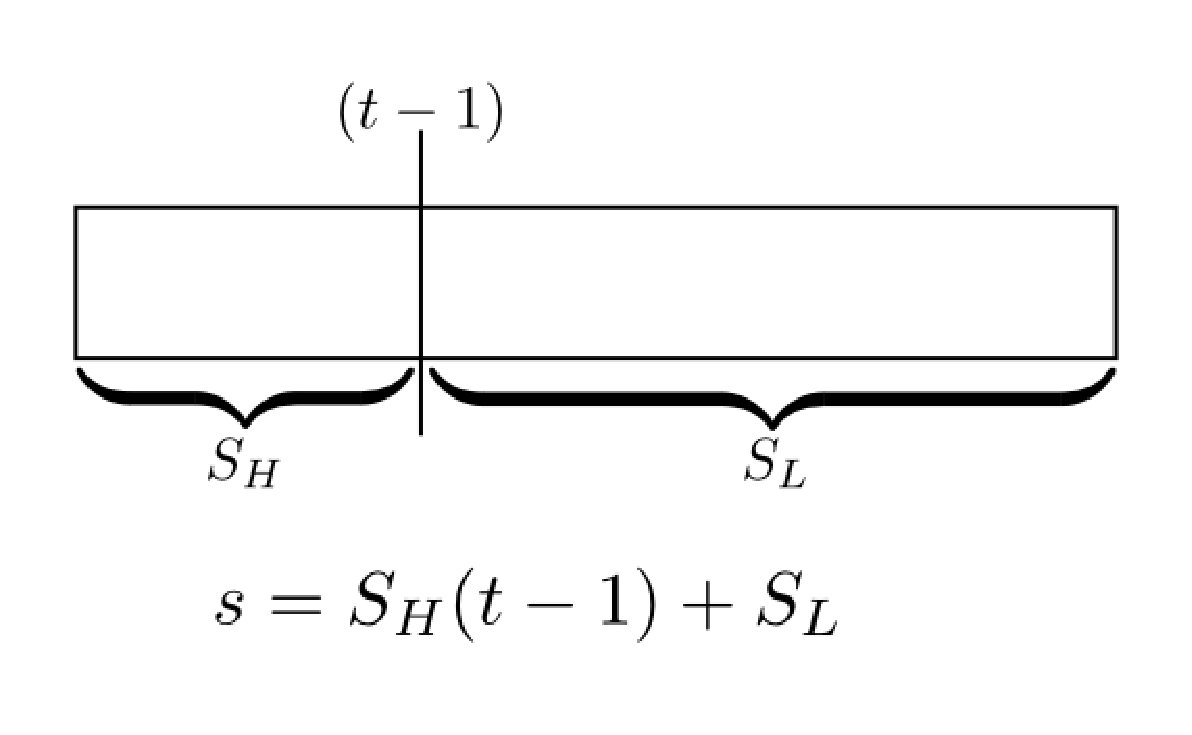
\includegraphics[width=0.7\linewidth, height=\textheight, keepaspectratio]{t_adic.eps}
	%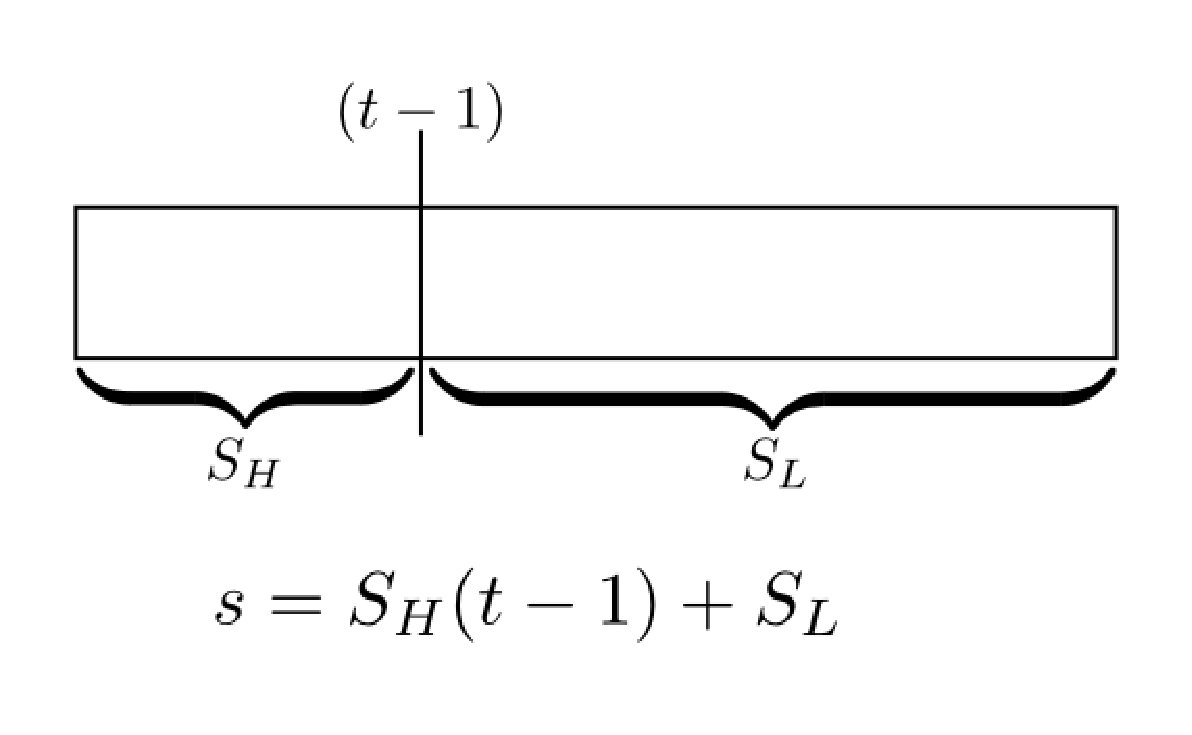
\includegraphics[width=0.7\columnwidth]{t_adic.eps}
	\caption{$(t-1)$ -adic representation of scalar $s$.}
	\label{fig:t_adic_chapter_g2scm_kss18}
\end{figure}

\begin{figure}[ht]
	\centering
	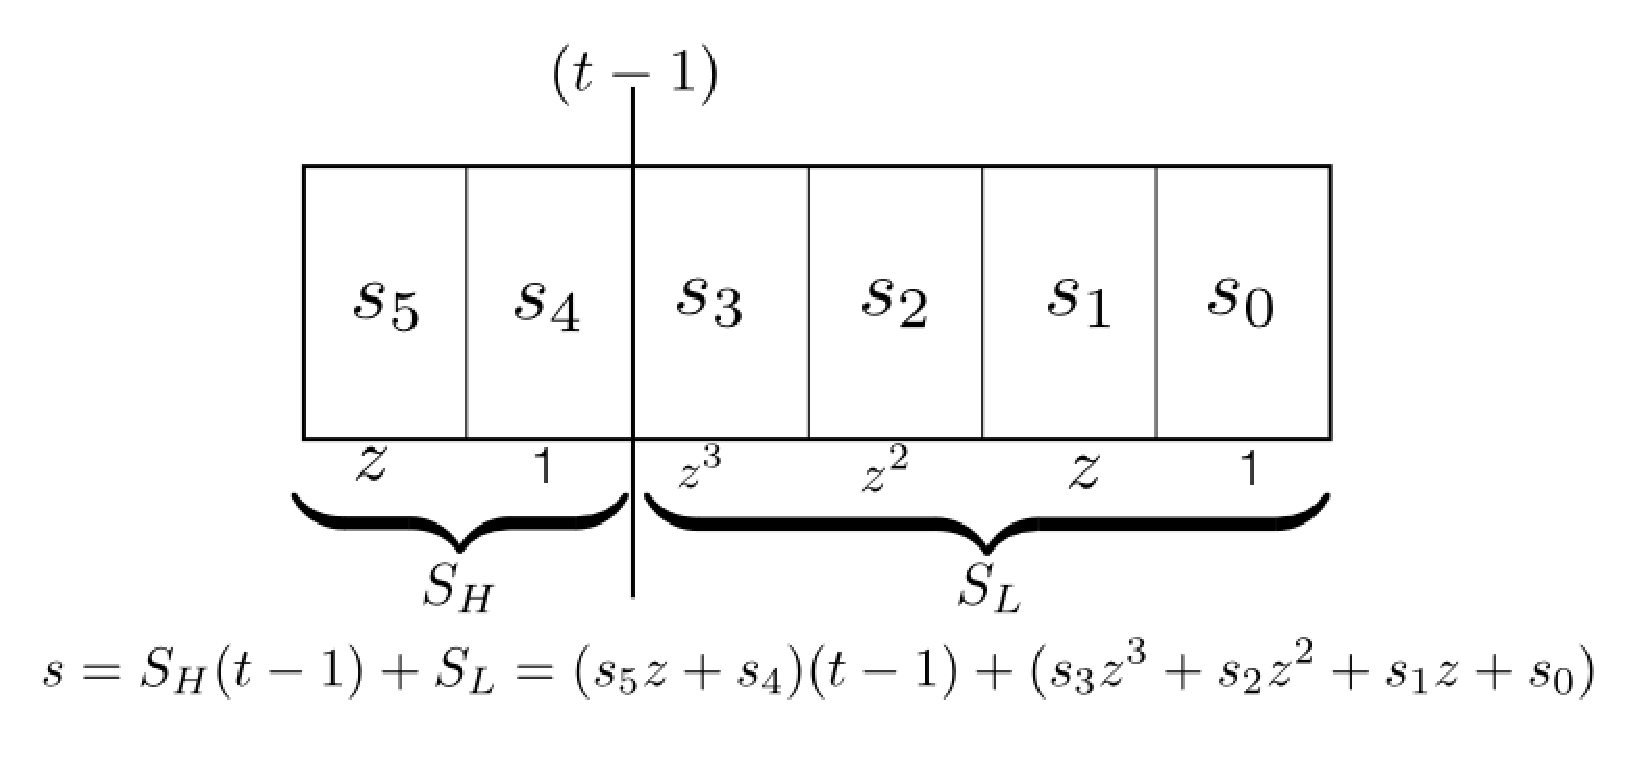
\includegraphics[width=\linewidth, height=\textheight, keepaspectratio]{z_adic.eps}
	\caption{$z$-adic and $(t-1)$-adic representation of scalar $s$.}
	\label{fig:z_adicl_chapter_g2scm_kss18}
\end{figure}

Figure \ref{fig:z_adicl_chapter_g2scm_kss18} shows the  $z$-adic representation of scalar $s$. 
In the previous work on Optimal-Ate pairing, Aranha et al. \cite{PAIRING:AFKMR12} derived a relation from the parameter setting of KSS-18 curve as follows:
\begin{equation}\label{eq:aranha_relationkss18_chapter_g2scm_kss18}
z+3p-p^4 \equiv 0 \bmod {r},
\end{equation}
where $z$ is the \textit{mother parameter} of KSS-18 curve which is about six times smaller than order $r$. 

Since $Q$ is mapped to its ismorphic sextic twisted rational point $Q'$, therefore we can consider scalar multiplication $[s]Q'$ where $0 \leq s < r$. $[s]Q'$ will be calculated in $\FQTH$ and eventually the result will be mapped to $\FQEN$ to get the final result. From \eqref{eq:kss_degree_chapter_g2scm_kss18} we know $r$ is the order of KSS-18 curve  where $[r]Q=\cal O$. Here, the bit size of $s$ is nearly equal to $r$. In KSS-18 curve $t$ is  $4/6$ times of  $r$. Therefore, let us first consider $(t-1)$-adic representation of $s$ as follows:
\begin{equation}\label{eq:t-1_adic_chapter_g2scm_kss18}
s =  S_H(t-1)+S_L,
\end{equation}
where $s$ will be separated into two coefficients $S_H$ and $S_L$. $S_L$ will be nearly equal to the size of $(t-1)$ and $S_H$ will be about half of $(t-1)$. 
In what follows, $z$-adic representation of $S_H$ and $S_L$ is given as:
\begin{eqnarray}\label{eq:eqn_scalar_mul_chapter_g2scm_kss18_Q}
S_H & =  & s_5+ s_4,\nonumber \\
S_L & = & s_3 z^3+s_2 z^2+s_1 z+s_0.\nonumber 
\end{eqnarray}
Finally $s$ can be represented as 6 coefficients as follows:
\begin{eqnarray}\label{eq:sclar_final_rep_chapter_g2scm_kss18}
s & =  & \sum_{i=0}^{3} s_iz^i + (s_4+s_5z)(t-1),\nonumber \\
s & = & (s_0+s_1z) + (s_2 +s_3z)z^2 +(s_4+s_5z)(t-1).
\end{eqnarray}

\subsection{Reducing Elliptic Curve Doubling in \texorpdfstring{$[s]Q'$}{[s]Q}}
Let us consider a scalar multiplication of $Q' \in \g2'$ in \eqref{eq:sclar_final_rep_chapter_g2scm_kss18} as follows:
\begin{equation}\label{eq:proposed_scm_1_chapter_g2scm_kss18}
[s]Q' =  (s_0+s_1z)Q' + (s_2 +s_3z)z^2Q'  +(s_4+s_5z)(t-1)Q'.
\end{equation}
In what follows, $z^2Q'$, $(t-1)Q'$ of \eqref{eq:proposed_scm_1_chapter_g2scm_kss18} is denoted as $Q_1'$ and $Q_2'$ respectively. From \eqref{eq:aranha_relationkss18_chapter_g2scm_kss18} and \eqref{eq:Q_rel2_chapter_g2scm_kss18} we can derive the $Q_1'$ as follows:
\begin{eqnarray}\label{eq:Q1_chapter_g2scm_kss18}
Q_1'& = & z^2 Q', \nonumber \\
& = & (9p^2-6p^5+p^8)Q',\nonumber \\
& = & 9\pi'^2(Q')-6\pi'^5(Q')+\pi'^8(Q').
\end{eqnarray}
where $\pi' (Q')$ is called the \textbf{skew Frobenius mapping} of rational point $Q' \in E'(\FQTH)$.
\eqref{eq:Q1_chapter_g2scm_kss18} is simplified as follows by utilizing the properties of cyclotomic polynomial.
\begin{eqnarray}\label{eq:Q11_chapter_g2scm_kss18}
Q_1' & = & 8\pi'^2(Q')-5\pi'^5(Q'),  \nonumber\\
& = & \pi'^2(8Q')-\pi'^5(5Q'). 
\end{eqnarray}
And from the \eqref{eq:Q_rel1_chapter_g2scm_kss18} and \eqref{eq:Q_rel2_chapter_g2scm_kss18}, $Q_2'$ is derived as,
\begin{equation}\label{eq:proposed_scm_2_chapter_g2scm_kss18}
Q_2' = \pi' (Q').
\end{equation}
Substituting \eqref{eq:Q11_chapter_g2scm_kss18} and \eqref{eq:proposed_scm_2_chapter_g2scm_kss18} in \eqref{eq:proposed_scm_1_chapter_g2scm_kss18}, the following relation is obtained. 
\begin{equation}\label{eq:proposed_scm_0_chapter_g2scm_kss18}
s[Q'] =  (s_0+s_1z)Q' + (s_2 +s_3z)Q_1' +(s_4+s_5z)Q_2'.
\end{equation}
Using $z \equiv -3p + p^4$ (mod $r$) from \eqref{eq:aranha_relationkss18_chapter_g2scm_kss18}, $z(Q')$ can be pre-computed as follows:
\begin{equation}
z(Q') = \pi'(-3Q') +\pi'^4(Q').
\end{equation}

Table \ref{table:pre-compute_chapter_g2scm_kss18} shows all the pre-computed values of rational points defined over $\FQTH$ for the proposed method. 
Pre-computed rational points are denoted inside angular bracket such as $<Q'+Q_2'>$ in this chapter. 

\renewcommand{\baselinestretch}{1.5}
\begin{table}[!ht]
	\centering
	\caption{13 pre-computed values of rational points.}
	\label{table:pre-compute_chapter_g2scm_kss18}
	\begin{tabular}{|c|c|}
		\hline 
		Pre-computed rational points & Skew Frobenius mapped rational points\\ 
		\hline 
		& $z(Q')$ \\ 
		\hline 
		$Q_1'$ & $z(Q_1')$  \\ 
		\hline 
		$Q_2'$ & $z(Q_2')$ \\ 
		\hline 
		$Q_1'+Q_2'$ & \quad  $ z(Q_1')+ z(Q_2') $ \quad \\ 
		\hline 
		$Q'+Q_2'$ & $ z(Q')+ z(Q_2') $ \\ 
		\hline 
		$Q'+Q_1'$ & $  z(Q')+ z(Q_1') $ \\ 
		\hline 
		\quad $Q'+Q_1'+Q_2'$ \quad  \quad &   \quad  $ z(Q')+ z(Q_1')+ z(Q_2')$  \quad \\ 
		\hline 
	\end{tabular} 
\end{table}
\renewcommand{\baselinestretch}{1.0}

\subsection{Skew Frobenius Map of \texorpdfstring{$\g{2}$}{} Points in KSS-18 Curve}
\index{KSS-18: Skew Frobenius map}
Similar to Frobenius mapping, skew Frobenius map is the $p$-th power over the sextic twisted isomorphic rational points such as  $Q' = (x',y')$ as 
follows:
\begin{equation}
\pi' : (x',y') \mapsto  (x'^p,y'^p)
\end{equation}
The detailed procedure to obtain the skew Frobenius map of $Q' = (x',y') \in \g2' \subset E'(\FQTH)$ is given bellow:
\begin{subequations}
	\begin{eqnarray}\label{eq:skew_x_prime_chapter_g2scm_kss18}
	\pi'(x') & = & (x')^p(i)^{1-p}(v)^{p-1}(\theta)^{p-1} \nonumber \\
	& = & (x')^p(i)^{1-p}(\theta^4)^{p-1} \nonumber \\
	& = & (x')^p (i^{-1})^pi(\theta^{p-1})^4 \nonumber \\
	& = & (x')^p (i^{-1})^pi(i^{\frac{p-1}{6}})^4  \mbox{\quad where $\theta^6=i$} \nonumber \\
	& = & (x')^p (i^{-1})^pi(i^{\frac{p-1}{6} -1}i)^4  \nonumber \\
	& = & (x')^p (i^{-1})^pi(i^{3\frac{\frac{p-7}{6}}{3}})^4i^4  \nonumber \\
	& = & (x')^p (i^{-1})^pi(2^{\frac{p-7}{18}})^42i  \mbox{\quad where $i^3=2$} \nonumber \\
	& = & (x')^p (i^{-1})^pi(2^{\frac{2p-14}{9}+1})i  \nonumber \\
	& = & (x')^p (i^{-1})^pi(2^{\frac{2p-5}{9}})i,
	\end{eqnarray}
	\begin{eqnarray}\label{eq:skew_y_prime_chapter_g2scm_kss18}
	\pi'(y') & = & (y')^p(i)^{1-p}(v)^{p-1} \nonumber \\
	& = & (y')^p (i^{-1})^pi(v^{6\frac{p-1}{6}})  \nonumber \\
	& = & (y')^p (i^{-1})^pi(i^{3\frac{p-1}{6}})  \nonumber \\
	& = & (y')^p (i^{-1})^pi2^{\frac{p-1}{6}}.
	\end{eqnarray}
\end{subequations}
Here $(i^{-1})^pi$, $(2^{\frac{2p-5}{9}})i$  and $2^{\frac{p-1}{6}}$ can be pre-computed. 

\subsection{Multi-Scalar Multiplication}
Applying the the multi-scalar multiplication technique in \eqref{eq:proposed_scm_0_chapter_g2scm_kss18} we can efficiently calculate the scalar multiplication in $\FQTH$. Figure \ref{eq:fig:z_sml_chapter_g2scm_kss18} shows an example of this multiplication.
Suppose in an arbitrary index, from left to right, bit pattern of $s_1$, $s_3$, $s_5$ is 101 and at the same index $s_0$, $s_2$, $s_4$ is 111.
Therefore we apply the pre-computed points $< z(Q')+z(Q_2') >$ and $<Q'+Q_1'+Q_2'>$ as ECA in parallel.
Then we perform ECD and move to the right next bit index to repeat the process until maximum length $z$-adic coefficient becomes zero.
\begin{figure}[!ht]
	\centering
	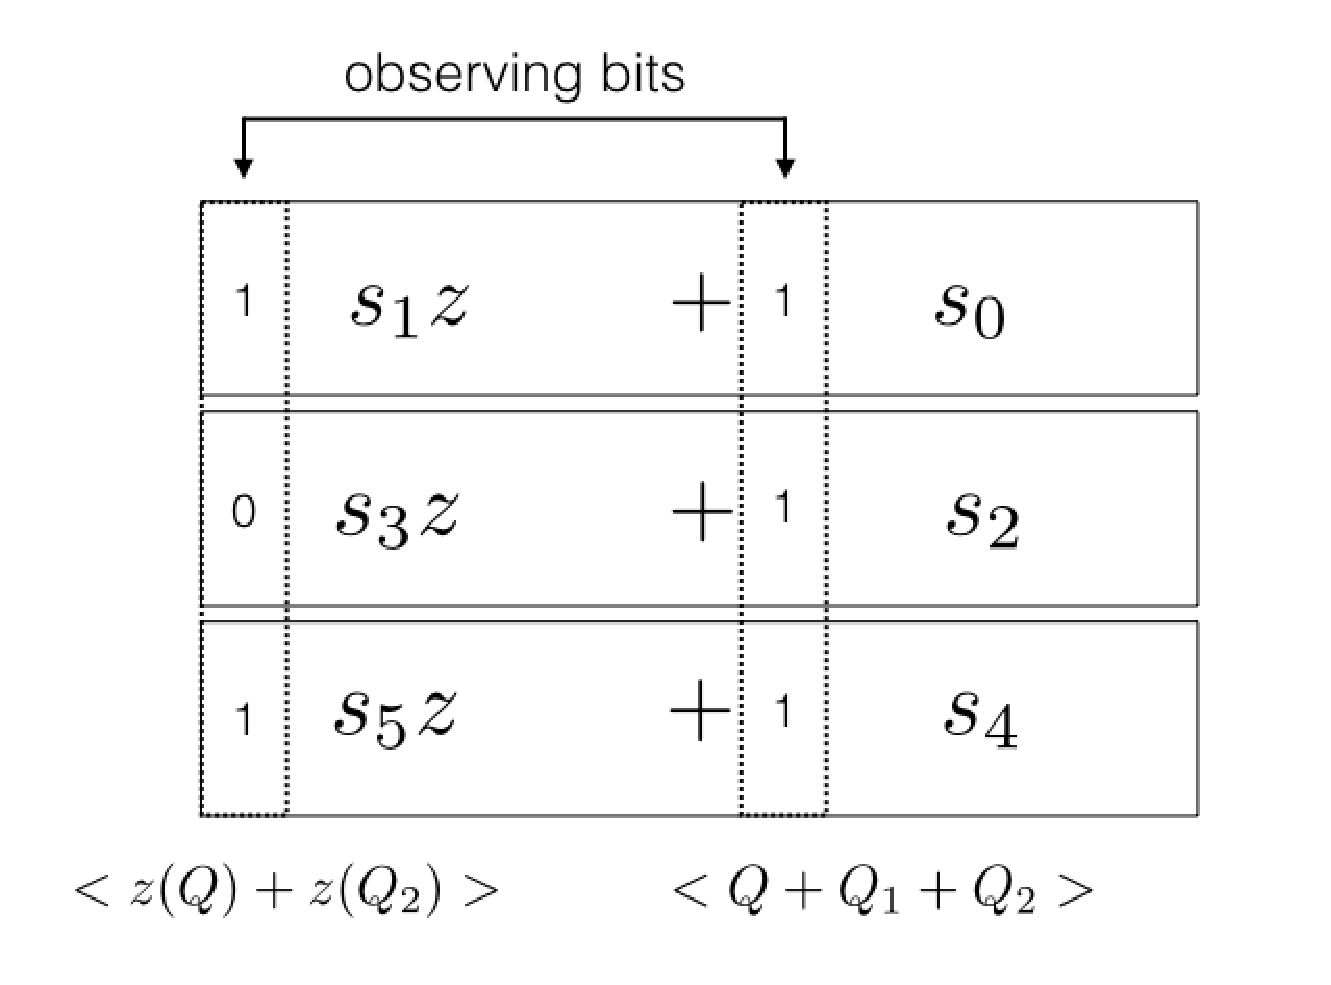
\includegraphics[width=0.8\linewidth, height=\textheight, keepaspectratio]{z_sm.eps}
	\caption{Multi-scalar multiplication of $s$ with Frobenius mapping.}
	\label{eq:fig:z_sml_chapter_g2scm_kss18}
\end{figure}

As shown in Figure \ref{eq:fig:z_sml_chapter_g2scm_kss18}, during scalar multiplication, we are considering 3 pair of coefficients of $z$-adic representation as shown in  \eqref{eq:sclar_final_rep_chapter_g2scm_kss18}. If we consider 6-coefficients for parallelization, it will require $2^6 \times 2$ pre-computed points. The chance of appearing each pre-computed point in the calculation will be once that causes redundancy.  

\subsubsection{Re-mapping Rational Points from \texorpdfstring{$E'(\FQTH)$}{} to  \texorpdfstring{$E(\FQEN)$}{}}
After the multi-scalar multiplication, we need to remap the result to $\FQEN$. For example let us consider re-mapping of $Q' =(x',y') \in E'(\FQTH)$ to $Q =(Av\theta,Bv) \in E(\FQEN)$. From \eqref{eq:thta2_4_chapter_g2scm_kss18}, \eqref{eq:thta_3_chapter_g2scm_kss18} and \eqref{eq:sextic_div_theta_chapter_g2scm_kss18} it can be obtained as follows:
\begin{subequations}
	\begin{eqnarray}
	x i^{-1}\theta^{4} & = & Av\theta, \nonumber \\
	y i^{-1}\theta^{3} & = & Bv, \nonumber
	\end{eqnarray}
\end{subequations}
which resembles that $Q= (Av\theta, Bv)$. Therefore it means that multiplying $i^{-1}$ with the $Q'$ coordinates and placing the resulted coefficients in the corresponding position of the coefficients in $Q$, will map $Q'$ to $Q$.
This mapping costs one $\FQTH$ inversion of $i$ which can be pre-computed and one $\Fp$ multiplication.

\section{Simulation Result}
This section shows the experimental result with the calculation cost.
In the experiment, we have compared the proposed method with three well-studied methods of scalar multiplication named binary method, sliding-window method, and non-adjacent form (NAF) method. 
The mother parameter $z$ is  selected according to the suggestion of Scott et al. \cite{IMA:Scott11} to obtain $p = 508 \approx 511$-bit and $r =  376 \approx 384$-bit  to simulate in 192-bit security level.
Table \ref{table:parameters_chapter_g2scm_kss18} shows the parameter settings considered for the simulation.

\renewcommand{\baselinestretch}{1.5}
\begin{table}[htb]
	\begin{center}
		\caption{Parameter settings used in the experiment.}
		%\resizebox{0.7\columnwidth}{!}{
		\begin{tabular}{|c|c|}
			\hline
			Defined KSS-18 curve & $y^2 = x^3 + 11$ \\ \hline
			Mother parameter $z$ & 65-bit \\ \hline
			Characteristics  $p(z)$ & 511-bit \\ \hline
			Order  $r(z)$ & 376-bit \\ \hline
			Frobenius trace $t(z)$ & 255-bit \\ \hline
			Persuadable security level & 192-bit \\ \hline
		\end{tabular}
		%}
		\label{table:parameters_chapter_g2scm_kss18}
	\end{center}
\end{table}
\renewcommand{\baselinestretch}{1.0}

Table \ref{table:comEnvironment_chapter_g2scm_kss18} shows the environment, used to experiment and evaluate the proposed method.  
\renewcommand{\baselinestretch}{1.5}
\begin{table}[!ht]
	\renewcommand{\arraystretch}{1.3}
	\centering
	\caption{ Computational environment.}
	\label{table:comEnvironment_chapter_g2scm_kss18}
	\resizebox{\columnwidth}{!}{
		\begin{tabular}{|c|c|c|}
			\hline 
			& PC & iPhone6s \\ 
			\hline \hline 
			CPU {\textsuperscript{*}} & \quad 2.7 GHz Intel Core i5 \quad & \quad Apple A9 Dual-core 1.84 GHz \quad \\ 
			\hline 
			Memory & 16 GB & 2 GB \\ 
			\hline 
			OS & Mac OS X 10.11.6 &  iOS 10.0 \\ 
			\hline 
			Compiler & gcc 4.2.1 & gcc 4.2.1 \\ 
			\hline 
			\quad Programming Language \quad  & C & Objective-C, C \\ 
			\hline 
			Library &  GMP 6.1.0 & GMP 6.1.0\\ 
			\hline 
			\multicolumn{3}{l}{\textsuperscript{*}\footnotesize{Only single core is used from two cores.}}\\
		\end{tabular} 
	}
\end{table}
\renewcommand{\baselinestretch}{1.0}

In experiment 100 random scalar numbers of size less than order $r$ ( 378-bit) is generated.
13  ECA counted for pre-computed rational points is taken into account while the average is calculated for the proposed method.
A window size of 4-bit is considered for the sliding-window method. 
Therefore 14 pre-computed ECA is required. 
Besides, the average execution time of the proposed method and the three other methods are also compared along with the operation count.

In what follows, ``\textit{\textbf{With isomorphic mapping}}'' refers that skew Frobenius mapping technique is applied for Binary, Sliding-window, and NAF methods. Therefore the scalar multiplication is calculated in $\FQTH$ extension field.
Moreover, for the Proposed method, it is skew Frobenius mapping with multi-scalar multiplication. 
On the other hand ``\textit{\textbf{Without isomorphic mapping}}'' denotes that Frobenius map is not applied for any of the methods.
In this case, all the scalar multiplication is calculated in $\FQEN$ extension field.

%\medskip\noindent
\renewcommand{\baselinestretch}{1.5}
\begin{table}[ht]
	\centering
	\caption{Comparison of average number of ECA and ECD for $\g{2}$ SCM in KSS-18.}
	\label{table:operationcount_chapter_g2scm_kss18}
	%\resizebox{\columnwidth}{!}{
	\begin{tabular}{l|l|l|}
		\cline{2-3}
		& \multicolumn{2}{l|}{Count of average number of ECA, ECD} \\ \hline
		\multicolumn{1}{|l|}{Methods}        & ECA      \quad     \quad       \quad \quad     \quad       \quad       & ECD                        \\ \hline
		\multicolumn{1}{|l|}{Binary}         & 186                         & 375                        \\ \hline
		\multicolumn{1}{|l|}{Sliding-window} & 102                         & 376                        \\ \hline
		\multicolumn{1}{|l|}{NAF}            & 127                         & 377                        \\ \hline
		\multicolumn{1}{|l|}{Proposed}       & 123                         & 64                         \\ \hline
	\end{tabular}
	%}
\end{table}
\renewcommand{\baselinestretch}{1.0}
In Table \ref{table:operationcount_chapter_g2scm_kss18} the operations of the \textit{Proposed} method are counted in $\FQTH$. On the other hand for Binary, Sliding-window and NAF method, the operations are counted in $\FQEN$.  The table clearly shows that in the \textit{Proposed} method requires about 6 times less ECD than any other methods.
The number of ECA has also reduced in the \textit{Proposed} method by about 30\% than binary method and the almost the same number of ECA of NAF. 

\renewcommand{\baselinestretch}{1.5}
\begin{table}[!ht]
	\centering
	\caption{Comparison of execution time in [ms] for scalar multiplication in KSS-18 curve.}
	\label{table:tab_executiontime_chapter_g2scm_kss18}
	\resizebox{\columnwidth}{!}{
		\begin{tabular}{|c|c|c|c|c|}
			\cline{2-5}
			\multicolumn{1}{c|}{} & 
			\multicolumn{4}{c|}{Execution time in [ms] }\\
			\cline{2-5}
			\multicolumn{1}{c|}{} & 
			\multicolumn{2}{c|}{With isomorphic mapping}&
			\multicolumn{2}{c|}{Without isomorphic mapping }\\
			\hline
			Methods & 
			PC &  iPhone6s &
			PC &  iPhone6s \\
			\hline
			Binary  
			&  $5.4 \times 10^1$  &  $8.4 \times 10^1$ 
			&  $1.2 \times 10^3$  &  $1.8 \times 10^3$ \\
			\hline
			Sliding-window 
			&  $4.8 \times 10^1$  &  $7.5 \times 10^1$ 
			&  $1.0 \times 10^3$  &  $1.6 \times 10^3$ \\
			\hline
			NAF
			&  $5.3 \times 10^1$  &  $7.7 \times 10^1$ 
			&  $1.6 \times 10^3$  &  $1.7 \times 10^3$ \\
			\hline
			Proposed
			&  $1.6 \times 10^1$  &  $2.4 \times 10^1$ 
			&  -  &  - \\
			\hline
			Multi-scalar  (only)
			&  -  &  -
			&  $3.4 \times 10^2$  &  $5.5 \times 10^2$ \\
			\hline
		\end{tabular}
	}
\end{table}
\renewcommand{\baselinestretch}{1.0}

Analyzing  Table \ref{table:tab_executiontime_chapter_g2scm_kss18}, we can find that when isomorphic mapping and skew Frobenius mapping is not adapted for  Binary, Sliding-window, and NAF, then the scalar multiplication of proposed method is more than 60 times faster than other methods. However when the isomorphic mapping is applied for the other methods, then our proposed technique is more than 3 times faster. Another essential comparison shows that when only multi-scalar multiplication is applied, then our proposed methods is about 20 times faster. 
In every scenario, our proposed method is faster than the other commonly used approaches.


The main focus of this experiment is to evaluate the acceleration ratio of scalar multiplication by applying the proposed approach on $\g2$ rational point group of  KSS curve of embedding degree 18. The experiment does not focus on efficiently implementing scalar multiplication for a particular environment. 

\section{Summary}
In this chapter, we have proposed an efficient method to calculate elliptic curve scalar multiplication using skew Frobenius mapping over KSS-18 curve in the context of pairing-based cryptography. 
Utilizing the skew Frobenius map along with the multi-scalar multiplication procedure, an efficient scalar multiplication method for KSS-18 curve is proposed in the chapter.
In addition to the theoretic proposal, this chapter has also presented a comparative simulation of the proposed approach with the plain binary method, sliding window method and non-adjacent form (NAF) for scalar multiplication. 
%The simulation shows that the proposed method is about 60 times faster than the plain implementation of other compared methods.
We have also applied $(t-1)$-adic and $z$-adic representation on the scalar and have applied multi-scalar multiplication technique to calculate scalar multiplication in parallel. 
We have evaluated and analyzed the improvement by implementing an experiment for the large size integer in 192-bit security level. 
According to the simulation result multi-scalar multiplication after applying skew Frobenius mapping in $\g2'$ can accelerate the scalar multiplication in $\g2 \subset E(\FQEN)$ by more than 60 times than scalar multiplication of $\g2$ rational point directly in $\FQEN$. 
 
\chapter{CANDAR 2016} 

        \title{Isomorphic Mapping for Ate-based Pairing over KSS Curve of Embedding Degree 18}

        
        

        Pairing based cryptography is considered as the next generation of security for which it attracts many researcher to work on faster and efficient pairing to make it practical. Among the several challenges of efficient pairing; efficient scalar multiplication of rational point defined over extension field of degree $k \geq 12$ is important. 
        %In Ate-based pairing, efficient arithmetic operation over the higher degree rational point groups reflects on the efficiency of the pairing calculation. Arithmetic over higher degree takes more time than arithmetic over lower degree groups. 
        However, there exists isomorphic rational point group defined over relatively lower degree extension field.
        %The important part of this process is mapping from higher degree group to lower degree isomorphic group and its reverse mapping. 
        Exploiting such property, this paper has showed a mapping technique between isomorphic rational point groups in the context of Ate-based pairing with Kachisa-Schaefer-Scott (KSS) pairing friendly curve of embedding degree $k = 18$. In the case of KSS curve, there exists sub-field sextic twisted curve that includes sextic twisted isomorphic rational point group defined over $\FQTH$. This paper has showed the mapping procedure from  certain $\FQEN$ rational point group to its sub-field isomorphic rational point group in $\FQTH$ and vice versa. This paper has also showed that scalar multiplication is about 20 times faster after applying the proposed mapping  which in-turns resembles that the impact of this mapping will greatly enhance the pairing operation in KSS curve.
        
        \section{Introduction}
         At the advent of this century, Sakai et al. \cite{sakai} and Joux et al. \cite{joux} independently proposed a cryptosystem based on elliptic curve pairing. Since then, pairing based cryptography has attracted many researchers and it has been considered as the basis of next generation security. Many researchers have proposed several innovative pairing based cryptographic applications such as ID-based encryption \cite{sakai}, broadcast encryption \cite{boradcast} and group signature authentication \cite{group_sign_1} that upsurge the popularity of pairing based cryptography.
        In such outcome, Ate-based pairings such as Ate \cite{ate}, R-ate \cite{r_ate}, Optimal-ate \cite{op_ate_p}, twisted Ate  \cite{twisted_ate} and $\chi$-Ate \cite{chibasedBN} pairings have gained much attention since they have achieved quite efficient pairing calculation. 
        There is no alternative of efficient and fast pairing calculation for deploying pairing-based cryptographic applications in practical case. 
        This paper focuses on a peripheral technique of Ate-based pairings with Kachisa-Schaefer-Scott (KSS) curve \cite{kss}. 
        
        In general, pairing is a bilinear map from two rational point group $\g1$ and $\g2$ to a multiplicative group $\g3$ \cite{Silverman}, typically denoted by $\g1 \times \g2 \rightarrow \g3$.
        In the context of Ate-based pairing, $\g1$, $\g2$ and $\g3$ are defined as follows:
        \begin{eqnarray}\label{eq:g_1}
        \g1 & = &  E(\F{p}{k}) [r] \cap \text{Ker}(\pi_p - [1]), \nonumber \\
        \g2 & = &  E(\F{p}{k}) [r] \cap \text{Ker}(\pi_p - [p]), \nonumber \\
        \g3 & = & \mF{p}{k}/(\mF{p}{k})^r, \nonumber
        \end{eqnarray}
        \begin{equation}
        \alpha : \g1 \times \g2 \rightarrow \g3,  \nonumber
        \end{equation}
        where $\alpha$ denotes Ate pairing. Pairings are often found in certain extension field $\FQK$, where $p$ is the prime number, also know as characteristics  and the minimum extension degree $k$ is called \textit{embedding} degree. 
        The rational points $E(\FQK)$ are defined over a certain pairing friendly curve $E$ of embedded extension field of degree $k$.
        This paper has considered Kachisa-Schaefer-Scott (KSS) \cite{kss} pairing friendly curves of emebdding degree $k=18$ described in \cite{taxonomy}. 
        
        %Pairing on KSS curve satisfies 192-bit security level which is considered to be the basis of next generation security. 
        In Ate-based pairing with KSS curve, where $k = 18$,  pairing computations are done in higher degree extension field $\FQEN$. However, KSS curves defined over $\FQEN$ have the sextic twisted isomorphism over $\FQTH$. Therefore we can execute computations in the sub-field $\FQTH$. Exploiting such a property, different arithmetic operation of Ate-based pairing can be efficiently performed in $\g2$. In this paper we have mainly focused on mapping $\g2$ rational point from extension field $\FQEN$ to its sextic twisted sub-field $\FQTH$ and its reverse procedure. 
        
        The advantage of such mapping is examined by performing scalar multiplication on $\g2 \subset E(\FQEN)$ rational point, since scalar multiplication is required repeatedly in cryptographic calculation. 
        We have considered sub-field sextic twisted curve of KSS curve, denoted as $E'$. It includes sextic twisted isomorphic rational point group denoted as $\g2' \subset E(\FQTH)$. In KSS curve, $\g2$ is defined over $\FQEN$ whereas its sub-field isomorphic group $\g2'$ is defined over $\FQTH$. Then the proposed mapping technique is applied to map rational points of $\g2$ to its isomorphic $\g2'$. After that the scalar multiplication in $\g2'$ performed and the resulted points are re-mapped to $\g2$ in $\FQEN$.
        The experiment result shows  that efficiency of binary scalar multiplication is increased by more than 20 times in sub-field sextic twisted curve than scalar multiplication in $\FQEN$ without applying proposed mapping. The mapping and remapping requires one bit wise shifting in $\Fp$, one $\FQTH$ inversion which can be pre-computed and one $\Fp$ multiplication; hence the mapping procedure has no expensive arithmetic operation.
        
        The rest of the paper is organized as follows. 
        The fundamentals of elliptic curve arithmetic, scalar multiplication along with KSS curve over $\FQEN$ extension field and \textit{sextic twist} of KSS curve are described in section \Romannum{2}.
        In section \Romannum{3}, this paper describes the isomorphic mapping between the rational point $Q$ and $Q'$ in details. The experimental result is presented in section \Romannum{4} which shows that our scalar multiplication on $\g2$ point can be accelerated by 20 times by applying the proposed mapping technique in KSS curve. Finally section \Romannum{5} draws the conclusion with some outline how this work can be enhanced more as a future work.
        
        \section{Preliminaries}
        In this section this paper briefly overviews the fundamentals of elliptic curve operations. Elliptic curve scalar multiplication is reviewed briefly. Pairing friendly curve of embedded degree $k=18$, i.e., KSS curve and its properties are introduced in combination  with its construction procedure by towering.
        % Rational point groups for Ate-based pairing is introduced briefly. 
        \subsection{Elliptic curve}
        Let $\Fp$ be a prime field and $\Fq$ be its extension field. An elliptic curve \cite{ecc_book} defined over $\Fp$ is generally represented by \textit{affine coordinates} \cite{Silverman} as follows;
        \begin{equation}\label{ec_curve}
        E/\Fp : y^2=x^3+ax+b,
        \end{equation}
        where $ 4a^3+27b^2 \neq 0$ and $a,b \in \Fp$. A pair of coordinates $x$ and $y$ that satisfy \eqref{ec_curve} are known as \textit{rational points} on the curve. 
        
        $E(\F{q}{k})$ denotes an elliptic curve group where the definition field is $\F{q}{k}$ and $\#E(\F{q}{k})$ denotes its order. When the definition field is prime field $\Fp$ then $\#E(\Fp)$ can be represented as,
        \begin{equation}\label{order}
        \#E(\Fp) = p+1-t,
        \end{equation} 
        where $t$ is called the Frobenius trace of $E(\Fp)$.
        
        Let $E(\f{p})$ be the set of all rational points on the curve defined over $\Fp$ and it includes the point at infinity denoted by $\mathcal{O}$. 
        The order of $\EFP$ is denoted by $\SEFP$ where $\EFP$ forms an additive group for the elliptic addition. The set of rational points over $\Fq$, including $\mathcal{O}$ satisfying \eqref{ec_curve} is denoted by $E(\Fq)$. The order of $E(\Fq)$ is denoted by $\#E(\Fq)$.
        
        Let us consider two rational points using affine coordinates as $P_1= (x_1, y_1)$, $P_2 = (x_2, y_2)$, and their addition $R = P_1 + P_2$, where $\textit{R} = (x_3, y_3)$ and $P_1, P_2, R \in E(\Fq)$. Then the $x$ and $y$ coordinates of $R$ are calculated as follows:
        
        \begin{subequations}
        \begin{eqnarray}\label{eq:point_add}
        x_3 & = & \lambda^2-x_1-x_2 ,\\
         y_3 & = &(x_1-x_3)\lambda - y_1, 
        \end{eqnarray}
        where \mbox{$\lambda$} is given as follows:
        \begin{equation}\label{eq:point_solpe}
        \textstyle \lambda = 
        \begin{cases}
         \textstyle \frac{y_2 - y_1}{ x_2 -x_1}; \quad \mbox{$P_1 \neq P_2$},\\
         \textstyle \frac{3x_1^2+a}{2y_1}; \quad  \mbox{$P_1 = P_2$},\\
        \end{cases}
        \end{equation}
        \end{subequations}
        $\lambda$ is the tangent at the point on the curve and $\cal O$ is the additive unity in $E(\f{q})$. When $P_1 \neq P_2$ then $P_1+P_2$ is called elliptic curve addition (ECA). If $P_1=P_2$ then $P_1+P_2=2P_1$, which is known as elliptic curve doubling (ECD). 
        %\subsubsection{Scalar multiplication.}
        
        Let $[s]P_1$ be the scalar multiplication for the rational point $P_1$ with scalar $s$ as,
        
        \begin{equation}\label{scalar_mul}
        [s]P_1 = \sum_{i=0}^{s-1} P_1, \quad \text{$0 \leq s < r$},
        \end{equation}
        where $r$ is the order of the target rational point group. If $s = r$, where $r$ is the order of the curve then $[r]P_1 = \mathcal{O}$. When $[s]P_1 = P_2$, if $s$ is unknown, then the solving $s$ from $P_1$ and $P_2$ is known as elliptic curve discrete logarithm problem (ECDLP). The security of elliptic curve cryptography depends on the difficulty of solving ECDLP.
        
        The binary method is a widely recognized method for calculating the elliptic curve scalar multiplication. Algorithm \ref{alg:bin} shows the binary scalar multiplication algorithm. This algorithm scans the bits of scalar $s$ from  most significant bit to least significant bit. When $s[i] = 1$, it will perform ECA and ECD otherwise only ECD will be calculated. But this method is not resistant to side channel attack \cite{sca}.  
        
         \begin{algorithm}[H]
          \caption{Left-to-right binary algorithm for elliptic curve scalar multiplication}
          \label{alg:bin}
          \DontPrintSemicolon
          \hspace{-3ex}
          \KwIn{ $P$, $s$}\;
          \hspace{-3ex}
          \KwOut{$[s]P$} \;%output
          \nl $T$ $ \leftarrow$ $0$ \;
          \nl \For{$i = \lfloor \log_2 s \rfloor$ {\bf to} $0$} {\;
                  $T \leftarrow T  + T$\;
             \If{ $s[i] = 1$}{
                  $ T \leftarrow T + P$\;
                    } }\;
          \nl \text{return} $T$\;
          \end{algorithm}
        
        On the other hand Montgomery ladder algorithm is said to be resistant of side channel attack. Algorithm \ref{alg:mont} shows the Montgomery ladder algorithm for scalar multiplication. Montgomery ladder has some similarity with binary method except in each iteration it performs ECA and ECD. 
        
         \begin{algorithm}[H]
          \caption{Montgomery ladder algorithm for elliptic curve scalar multiplication}
          \label{alg:mont}
          \DontPrintSemicolon
          \hspace{-3ex}
          \KwIn{ $P$, $s$}\;
          \hspace{-3ex}
          \KwOut{$[s]P$} \;%output
          \nl $T_0$ $ \leftarrow$ $0$, $T_1$ $\leftarrow$ $P$ \;
          \nl \For{$i = \lfloor \log_2 s \rfloor$ {\bf to} $0$} {\;
         
             \If{ $s[i] =1$}{
                  $ T_0 \leftarrow T_0 + T_1$\;
                    $T_1 \leftarrow T_1 + T_1$\;
                    }
                    {\ElseIf{$s[i] = 0$}{ 
                    $T_1 \leftarrow T_0 + T_1$\;
                           $T_0 \leftarrow T_0 + T_0$\;}
                }
          }\;
          \nl \text{return} $T_0$\;
        \end{algorithm}
        This paper has considered left-to-right binary scalar multiplication for evaluating the efficiency of the proposed mapping operation. But from the view point of security binary method is vulnarable to side channel attack. Therefore this paper has also experimented with Montgomery ladder \cite{Silverman} for scalar multiplication evaluation.
        
        \subsection{KSS curve}
        Kachisa-Schaefer-Scott (KSS) curve \cite{kss} is a non super-singular pairing friendly elliptic curve of embedding degree 18, defined over $\FQEN$ as follows: 
        \begin{equation}\label{eq:KSS_curve}
        E/\FQEN:Y^2=X^3+b, \quad \mbox{$b \in \Fp$},
        \end{equation}
        where $b \neq 0$ and $X,Y \in \FQEN$. Its characteristic $p$, Frobenius trace $t$ and order $r$ are given systematically by using an integer variable $u$ as follows:
        \begin{subequations}
        \begin{eqnarray}
        p(u) &= & (u^8 +5u^7 +7u^6 +37u^5 +188u^4 +259u^3 \nonumber \\
        & & + 343u^2 +1763u+2401)/21,\\\label{eq:kss_char}
        r(u) &= &(u^6 + 37u^3 + 343)/343,\label{eq:kss_degree}  \\
        t(u) &=& (u^4 + 16u + 7)/7, \label{eq:kss_trace} 
        \end{eqnarray}
        \end{subequations} 
        
        where $u$ is such that $u \equiv 14$ (mod $42$) and the $\rho$ value is $\rho = (\log_2 p/\log_2 r) \approx 1.33$.
        
        %The order of rational points $\#E(\FQEN)$ on KSS curve can be obtained by the following relation.
        %\begin{equation}\label{eq:order_relation}
        %\#E(\FQEN) = p^{18}+1-t_{18},
        %\end{equation}
        %where $t_{18} = \alpha^{18}+\beta^{18}$ and $\alpha$, $\beta$ are complex numbers such that $\alpha+\beta = t$ and $\alpha\beta=p$.
        
        
        \subsection{$\FQEN$ extension field arithmetic}
        In pairing, arithmetic  operations are performed in higher degree extension fields, such as $\FQK$  for moderate value of $k$ \cite{Silverman}. Concequently, such higher extension field needs to be constructed as tower of extension fields \cite{const_ext} to perform arithmetic operation cost effectively.
        
        This paper has  represented extension field $\FQEN$ as a tower of sub-field to improve arithmetic operations. It has also used irreducible binomials introduced by Bailey et al. \cite{JC:BaiPaa01}. In what follows, this paper considers $3|(p-1)$ and $c$ is a quadratic and cubic non residue in $\Fp$. In context  of KSS-curve \cite{kss}, where $k=18$, $\FQEN$ is constructed as tower field with irreducible binomial as follows:
        \begin{equation}\label{eq:KSS_towering}
        \begin{cases}
        \F{p}{3} = \F{p}{}[i]/(i^3-c),  \\ 
        \F{p}{6} = \F{p}{3}[v]/(v^2-i),  \\ 
        \F{p}{18} = \F{p}{6}[\theta]/(\theta^3-v), \\ 
        \end{cases}
        \end{equation}
        where $c = 2$ is considered to be the best choice for efficient arithmetic.
        From the above towering construction we can find that $i=v^2=\theta^6$, where $i$ is the basis element of the base extension field $\FQTH$. 
        In the previous work of Aranha et al. \cite{PAIRING:AFKMR12}, explained the base extension field $\FQTH$ for the \textit{sextic twist} of KSS curve.
        
        \subsection{\g1, \g2 and \g3 groups.} In the context of pairing-based cryptography, especially on KSS curve, three groups $\g1, \g2$ and $\mathbb{G}_3$ are considered. From \cite{mori}, we define $\g1$, $\g2$ and $\g3$ as follows:
        \begin{eqnarray}\label{eq:g1}
        \g1 & = &  E(\F{p}{18}) [r] \cap \text{Ker}(\pi_p - [1]), \nonumber \\
        \g2 & = &  E(\F{p}{18}) [r] \cap \text{Ker}(\pi_p - [p]), \nonumber \\
        \g3 & = & \mF{p}{18}/(\mF{p}{18})^r, \nonumber
        \end{eqnarray}
        \begin{equation}
        \alpha : \g1 \times \g2 \rightarrow \g3,
        \end{equation}
        where $\alpha$ denotes Ate pairing. In the case of KSS curve, $\g1, \g2$ are rational point groups and $\mathbb{G}_3$ is the multiplicative group in $\FQEN$. They have the same order $r$. 
        
        \subsection{Sextic twist of KSS curve}
        %When the embedding degree $k = 2e$, where $e$ is positive integer, from \eqref{ec_curve} the quadratic twisted elliptic curve $E'_2$ is given as follows:
        %\begin{equation}\label{eq:quad_twist}
        %E'_2:y^2=x^3+az^{-2}+bz^{-3}, \quad a,b \in \F{p},
        %\end{equation}
        %where $z$ is a quadratic non residue in $\F{p}{e}$. Then, between $E'_2(\F{p}{e})$ and $E(\F{p}{2e})$, the following isomorphism is given.
        %\begin{eqnarray}
        %\psi_2 : \begin{cases}
        %E'_2(\F{p}{e}) \rightarrow E(\F{p}{2e}),\\
        %(x,y) \quad \mapsto (xz,yz^{3/2}),
        %\end{cases}
        %\end{eqnarray}
        %where $x, y$ are the coordinates of rational point. In this case, $E'_2$ is called \textit{quadratic-twisted} curve. In the same, 
        
        When the embedding degree $k = 6e$, where $e$ is positive integer, \textit{sextic} twist is given as follows:
        \begin{eqnarray}
        E:  \quad y^2 & = & x^3+b, \quad b \in \Fp, \\
        E'_6: \quad y^2 & =  & x^3+bz^{-1},
        \end{eqnarray}  
        where $z$ is a quadratic and cubic non residue in $E(\F{p}{e})$ and $3|(p^e-1)$.  Isomorphism between $E'_6(\F{p}{e})$ and $E(\F{p}{6e})$, is given as follows:
        \begin{eqnarray}
        \psi_6 : \begin{cases}
        E'_6(\F{p}{e}) \rightarrow E(\F{p}{6e}),\\
        (x,y) \quad \mapsto (xz^{1/2},yz^{1/2}).
        \end{cases}
        \end{eqnarray}
        In context of Ate-based pairing for KSS curve of embedding degree 18, sextic twist is considered to be the most efficient. This papers considers mapping of sextic twisted sub-field isomorphic group of $\FQEN$. 
        
        \section{Isomorphic mapping between $Q$ and $Q'$}
        This section introduces our proposal of mapping procedure of $\g2$ rational point group to its sextic twisted isomorphic group $\g2'$ for Ate-based pairing with KSS curve. 
        
        Figure \ref{fig:sextic} shows an overview of sextic twisted curve $E'(\FQTH)$ of $E(\FQEN)$.
        \begin{figure*}
        \centering
        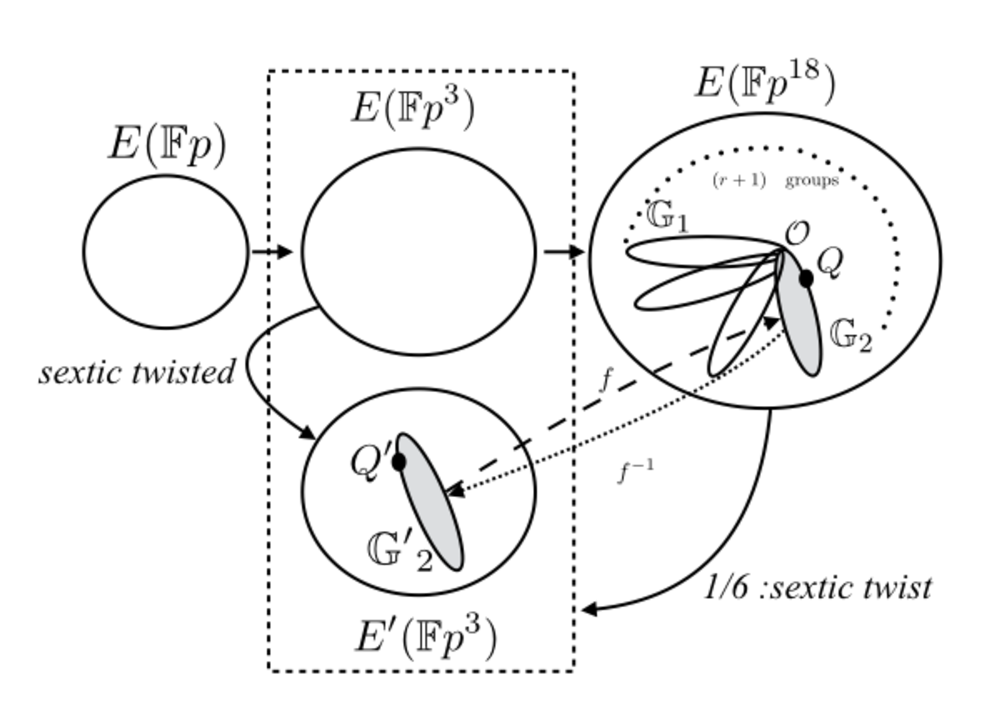
\includegraphics[width=3.5in]{twist.eps}
        \caption{\textit{sextic twist} in KSS curve.}
        \label{fig:sextic}
        \end{figure*}
        Let us consider $E$ is the KSS curve in base field $\FQTH$  and $E'$ is sextic twist of $E'$ given as follows: 
        \begin{eqnarray}
        E:y^2 & = &x^3+b,\\
        E':y^2 & = & x^3+bi, \label{eq:KSS_Twist}
        \end{eqnarray}
        where $b \in \Fp$; $x, y, i \in \FQTH$ and basis element $i$ is the quadratic and cubic non residue in $\FQTH$.
        
        In context of KSS curve, let us consider a rational point $Q\in \g2 \subset E(\F{p}{18})$.
        $Q$ has a  special vector representation with 18 $\Fp$ elements for each $x_Q$ and $y_Q$ coordinates.
        Figure \ref{fig:Q_structure} shows the structure of the coefficients of $Q \in \FQEN$ and its sextic twisted isomorphic rational point $Q' \in \FQTH$ in KSS curve.
        \begin{figure*}
        \centering
        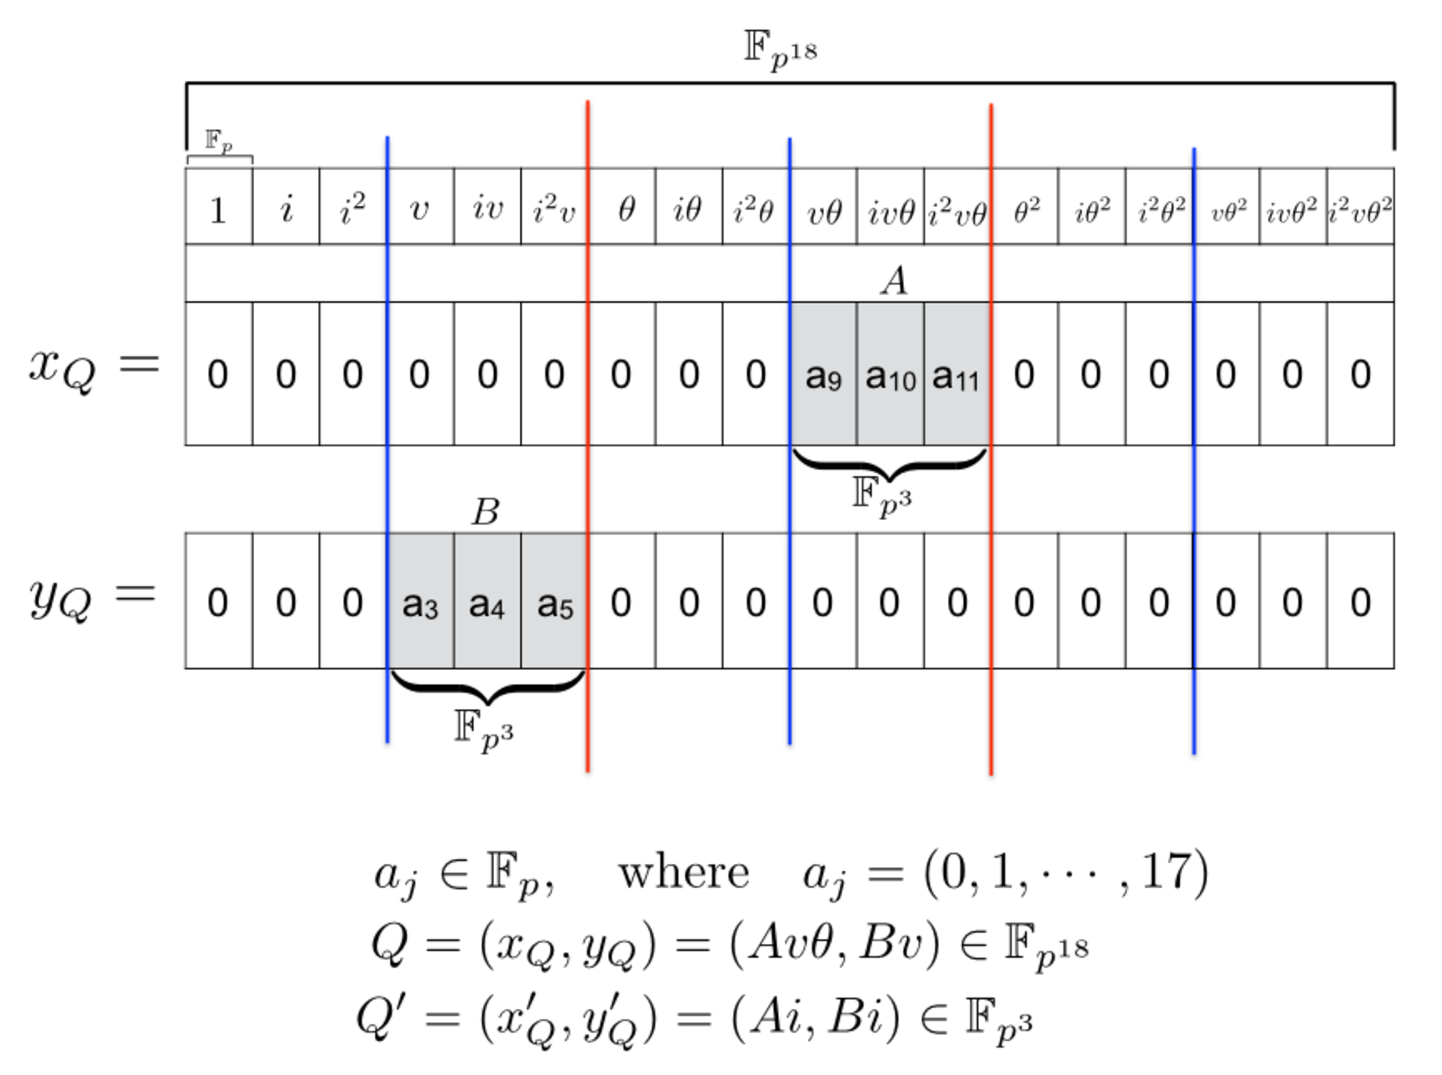
\includegraphics[width=4.5in]{structure.eps}
        \caption{ $Q \in \FQEN$ and its sextic twisted isomorphic rational point $Q' \in \FQTH$ structure in KSS curve.}
        \label{fig:Q_structure}
        \end{figure*}
        Among 18 elements, there are 3 continuous nonzero $\Fp$ elements. The others are zero.
        However the set of these nonzero elements belongs to $\FQTH$. 
        
        This paper considers the mother parameter of KSS curve $u=65$-bit and characteristics $p=511$-bit. In such consideration, $Q$ is given as $Q = (Av\theta, Bv)$,  showed in Figure \ref{fig:Q_structure}, where $A, B \in \FQTH$ and $v$ and $\theta$ are the basis elements of $\F{p}{6}$ and $\FQEN$ respectively. 
        
        Let us consider the sextic twisted isomorphic sub-field rational point of $Q$ as $Q' \in \g2' \subset E'(\F{p}{3})$.
        Considering $x'$ and $y'$ as the coordinates of $Q'$, we can map the rational point $Q = (Av\theta, Bv)$  to the rational point  $Q' = (x',y')$ as follows.
        
        Multiplying both side of \eqref{eq:KSS_Twist} with $\theta^{-6}$, where $i=\theta^6$ and $v = \theta^3$.
        \begin{equation}\label{eq.sextic_div_theta}
        E':  \Big(\frac{y}{\theta^3}\Big)^2  = \Big(\frac{x}{\theta^2}\Big)^3+ b.
        \end{equation}
         $\theta^{-2}$ of  \eqref{eq.sextic_div_theta} can be represented as follows:
         \begin{subequations}
         \begin{eqnarray}
         \theta^{-2} & = & i^{-1}i \theta^{-2}, \nonumber \\
         &  = & i^{-1}\theta^{4}, \label{thta2_4}
         \end{eqnarray}
         and multiplying $i$ with both sides.
         \begin{equation} \label{the4_2}
         \theta^4 = i\theta^{-2}.
         \end{equation}
        Similarly $\theta^{-3}$ can be represented as follows:
         \begin{eqnarray}
         \theta^{-3} & = & i^{-1}i \theta^{-3} \nonumber \\
         &   = & i^{-1}\theta^{3}.\label{thta_3} 
         \end{eqnarray}
         Multiplying $i$ with both sides of \eqref{thta_3} we get $\theta^3$ as,
         \begin{equation}\label{thta_3_3}
         \theta^3 = i\theta^{-3},
         \end{equation}
         \end{subequations}
        
        \subsubsection{$Q$ to $Q'$ mapping}
        Let us represent $Q = (Av\theta, Bv)$  as follows:
        \begin{equation}\label{18_to3}
        Q  =  (A\theta^4, B\theta^3), \quad \text{where $v=\theta^3$}.
        \end{equation}
        From \eqref{the4_2} and \eqref{thta_3_3}, we substitute $ \theta^4 = i\theta^{-2}$ and $\theta^3 = i\theta^{-3}$  in \eqref{18_to3}  as 
        follows:
        \begin{equation}\label{18_to3.1}
        Q  =  (Ai\theta^{-2}, Bi\theta^{-3}),
        \end{equation}
        where $Ai = x'$ and $Bi = y'$ are the coordinates of $Q' =(x',y') \in \FQTH$. Which implies that we can map $Q \in \FQEN$ to $Q' \in \FQTH$ by first selecting the $3$ nonzero $\Fp$ coefficients of each coordinates of $Q$. Then these nonzero $\Fp$ elements form an $\FQTH$ element. After that multiplying the basis element $i$ with that $\FQTH$ element, we get the final $Q' \in \FQTH$. From the structure of $\FQEN$, given in \eqref{eq:KSS_towering}, this mapping has required no expensive arithmetic operation.  Multiplication by the basis element $i$ in $\FQTH$ can be done by 1 bit wise left shifting since $c=2$ is considered for towering in \eqref{eq:KSS_towering}.
        
        \subsubsection{$Q'$ to $Q$ mapping}
         The reverse mapping $Q' =(x',y') \in \FQTH$ to $Q =(Av\theta,Bv) \in \FQEN$ can be obtained as from \eqref{thta2_4}, \eqref{thta_3} and \eqref{eq.sextic_div_theta} as follows:
         \begin{subequations}
         \begin{eqnarray}
         x i^{-1}\theta^{4} & = & Av\theta, \nonumber \\
         y i^{-1}\theta^{3} & = & Bv, \nonumber
         \end{eqnarray}
         \end{subequations}
          which resembles that $Q= (Av\theta, Bv)$. Therefore it means that multiplying $i^{-1}$ with the $Q'$ coordinates and placing the resulted coefficients in the corresponding position of the coefficients in $Q$, will map $Q'$ to $Q$.
        This mapping costs one $\FQTH$ inversion of $i$ which can be pre-computed and one $\Fp$ multiplication.
        
        
        \section{Result Analysis}
        In order to determine the advantage of the proposal, first we have applied the proposed mapping technique to map rational point $Q \in \g2 \subset E(\F{p}{18})$ to its isomorphic point $Q' \in \g2' \subset E'(\F{p}{3})$. After that we performed the scalar multiplication of $Q'$. Then the resulted points are re-mapped to $\g2$ in $\FQEN$. On the other hand we performed scalar multiplication of $Q$ without mapping. In the experiment, 100 scalar numbers of size (about 377-bit) less than order $r$ is generated randomly and then scalar multiplication is calculated for both case. Average value of execution time is considered for comparison.
        The comparative result is shown in Table \ref{tab_opeation}.
        
        In the experiment, mother parameter $u$ is also selected accordingly to find out $\g2$ rational point $Q$. In addition $p=511$-bit is considered, since Scott et al. \cite{kss_param} has proposed the size of the characteristics $p$ to be 508 to 511-bit with order $r$ of 384-bit for 192-bit security level.
        
        In the experiment, KSS curve over $\FQEN$ is given as $y^2 = x^3 + 11$, considering the following parameters
        \begin{eqnarray}
        u & = & 65   \mbox{-bit},  \nonumber \\ 
        p  & = & 511 \mbox{-bit},  \nonumber \\ 
        r  & = & 378 \mbox{-bit} ,\nonumber \\ 
        t  & = & 255  \mbox{-bit}. \nonumber
        \end{eqnarray}
        
        Table \ref{tab1} shows the experiment environment, used to evaluate usefulness of the proposed mapping.  
        \renewcommand{\baselinestretch}{1.5}
        \begin{table*}
        \renewcommand{\arraystretch}{1.3}
        \centering
        \caption{ Computational Environment}
        \label{tab1}
        \begin{tabular}{|c|c|c|}
        \hline 
        • & PC & iPhone6s \\ 
        \hline \hline 
        CPU {\textsuperscript{*}} & \quad 2.7 GHz Intel Core i5 \quad & \quad Apple A9 Dual-core 1.84 GHz \quad \\ 
        \hline 
        Memory & 16 GB & 2 GB \\ 
        \hline 
        OS & Mac OS X 10.11.4 &  iOS 9.3.1 \\ 
        \hline 
        Compiler & gcc 4.2.1 & gcc 4.2.1 \\ 
        \hline 
        \quad Programming Language \quad  & C & Objective-C, C \\ 
        \hline 
        Library & GNU MP \cite{gmp} & GNU MP \\ 
        \hline 
        \multicolumn{3}{l}{\textsuperscript{*}\footnotesize{Only single core is used from two cores.}}\\
        \end{tabular} 
        \end{table*}
        \renewcommand{\baselinestretch}{1.0}
        
        \renewcommand{\baselinestretch}{1.5}
        \begin{table*}
        %\renewcommand{\arraystretch}{1.3}
        \centering
        \caption{ Comparative result of average execution time in [ms] for scalar multiplication}
        \label{tab_opeation}
        \begin{tabular}{|c|c|c|c|}
        \hline
         & \multicolumn{3}{|c|}{\quad Average execution time [ms] comparison \quad} \\ \hline
        & PC & \multicolumn{2}{|c|}{iPhone 6s}  \\ 
         \hline \hline
         & \quad Execution time \quad & \multicolumn{2}{|c|}{\quad Execution time}\\ 
         \hline
        Binary method  with mapping &  $5.4 \times 10^1 $  &  \multicolumn{2}{|c|} { $6.4 \times 10^1$}\\ \hline
        Binary method  without mapping  &  $1.1 \times 10^3$  &  \multicolumn{2}{|c|} { $1.2 \times 10^3$}\\ \hline
        Montgomery ladder  with mapping &  $6.8 \times 10^1 $  &  \multicolumn{2}{|c|} { $8.4 \times 10^1$}\\ \hline
        Montgomery ladder  without mapping  &  $1.5 \times 10^3$  &  \multicolumn{2}{|c|} { $1.6 \times 10^3$}\\ \hline
        \end{tabular} 
        \end{table*}
        \renewcommand{\baselinestretch}{1.0}
        
        Analyzing  Table \ref{tab_opeation}, we can find that scalar multiplication using the proposed  mapping technique  is more than 20 times faster than scalar multiplication without the proposed mapping. It this experiment we used binary method and Montgomery ladder for scalar multiplication in both case. In the previous work of Nogami et al. \cite{nogami}, has showed the procedure to apply Frobenious mapping on twisted elliptic curve for Ate-based pairing. This multiplication can be done more efficiently if skew Frobenius mapping is applied on sextic twisted isomorphic rational point after applying the proposed mapping. 
        
        In the experiment we have used two execution environments; such as PC and iPhone with different CPU frequencies. In both environments only one processor core is utilized. The result also shows that the ratio of execution time of PC and iPhone without mapping  of both methods is about 0.9. On the other hand the ratio of execution time with mapping  of both methods is about 0.8. But the ratio of CPU frequencies of  iPhone and PC is about $1.84 / 2.7 \approx 0.68$. Since PC and iPhone has different processor architectures therefore it's frequency ratio has no relation with the execution time ratio. 
        
        The main focus of this experiment is to evaluate the  acceleration ratio of scalar multiplication by applying the proposed mapping on $\g2$ rational point group of  KSS curve of embedding degree 18. The experiment does not focus on efficiently implementing scalar multiplication for certain environment. There are other pairing friendly curves such as BLS-12, BLS-24 \cite{taxonomy} where sextic twist is available. We will try to apply the proposed mapping on those curves as our future work.
        
        \section{Conclusion and future work}
        In this paper we have proposed mapping procedure of $\g2$ rational point group to its sextic twisted sub-field isomorphic rational point group $\g2'$  and its reverse mapping on KSS curve in context of Ate based pairing. 
        We have also presented the advantages of such mapping by applying binary scalar multiplication and Montgomery ladder on sextic twisted isomorphic rational points in $\g2'$. 
        Then result of  scalar multiplication in $\g2'$ can accelerate the scalar multiplication in $\g2 \subset E(\FQEN)$ by more than 20 times than scalar multiplication of $\g2$ rational point directly in $\FQEN$. In the previous work of Sakemi et al. \cite{sakemi_skew} has proposed skew Frobenious map for $\g1$ rational point defined over BN curve. As a future work we would like to apply such approach on $\g1$ rational point defined over KSS curve. Together with the proposed mapping and the skew Frobenius mapping of $\g1$ will remarkably accelerate scalar multiplication over KSS curve in the context of pairing based cryptography.  
        
        %As a future work we would like to enhance the scalar multiplication in  sub-field isomorphic rational point group by applying Frobenius mapping and some multi-scalar multiplication technique.  
        
        
        \section*{Acknowledgment}
        This work was partially supported by the Strategic Information and Communications R\&D Promotion Programme (SCOPE) of Ministry of Internal Affairs and Communications, Japan.
        
        
         
\chapter{ICISC 2016} 
\chapter{Improved Optimal-Ate Pairing over KSS-18 Curve} 
\label{ch:optate_kss18_icisc2016}

\section{Introduction}
\label{ch:icisc2016:intro}

\subsection{Background and Motivation}
\label{sec:ch:icisc:bac_motivation}
From the very beginning of the cryptosystems that utilizes elliptic curve pairing; proposed independently by Sakai et al. \cite{EPRINT:SakKas03} and Joux \cite{JC:Joux04}, has unlocked numerous novel ideas to researchers. 
Many researchers tried to find out security protocol that exploits pairings to remove the need for certification by a trusted authority. 
In this consequence, several original pairing-based encryption schemes such as ID-based encryption scheme by  Boneh and Franklin \cite{C:BonFra01} and group signature authentication by Nakanishi et al. \cite{AC:NakFun05} have come into the focus. 
In such outcome, Ate-based pairings such as Ate \cite{DBLP:reference/crc/2005ehcc}, Optimal-Ate \cite{DBLP:journals/tit/Vercauteren10}, twisted Ate \cite{EPRINT:MKHO07},  R-ate \cite{r_ate}, and $u$-Ate \cite{PAIRING:NASKM08} pairings and their applications in cryptosystems have caught much attention since they have achieved quite efficient pairing calculation.
However, it has always been a challenge for researchers to make pairing calculation more efficient for being used practically as pairing calculation is regarded as a quite time-consuming operation. 

\subsection{General Notation}
\label{sec:ch:icisc:notation}
As aforementioned, pairing is a bilinear map from two rational point groups $\g1$ and $\g2$ to a multiplicative group $\g3$ \cite{Silverman}.
Bilinear pairing operation consists of two predominant parts,  named as Miller's algorithm and final exponentiation.
In  the case of  Ate-based pairing using KSS-18 pairing-friendly elliptic curve of embedding degree $k=18$,  the bilinear map is denoted by $\g1 \times \g2 \rightarrow \g3$,
The groups $\g1 \subset E(\FQ)$, $\g2 \subset E(\FQEN)$ and $\g3  \subset \mathbb{F}^*_{p^{18}}$ and  $p$ denotes the characteristic of $\Fp$.
The elliptic curve $E$ is defined over the extension field $\FQEN$. 
The rational point in $\g2 \subset E(\FQEN)$ has a unique vector representation where out of 18 $\Fp$ coefficients, continuously 3 of them are non-zero, and the others are zero. 
By utilizing such representation along with the sextic twist and isomorphic mapping in the subfield of $\FQEN$, this chapter has computed the elliptic curve doubling and elliptic curve addition in the Miller's algorithm as $\FQTH$ arithmetic without any explicit mapping from $\FQEN$ to $\FQTH$.

\subsection{Contribution}
\label{sec:ch:icisc:contriv_outline}
This chapter proposes \textit{pseudo 12-sparse multiplication} in affine coordinates for line evaluation in the Miller's algorithm by because multiplying or dividing the result of Miller's loop calculation by an arbitrary non-zero $\Fp$ element does not change the result as the following final exponentiation cancels the effect of multiplication or division. 
Following the division by a non-zero $\Fp$ element, one of the 7 non-zero $\Fp$ coefficients (which is a combination of 1 $\Fp$ and 2 $\FQTH$ coefficients) becomes 1 that yields calculation efficiency.
The calculation overhead caused by the division is canceled by isomorphic mapping with a quadratic and cubic residue in $\Fp$.
This chapter does not end by giving only the theoretic proposal of improvement of Optimal-Ate pairing by pseudo 12-sparse multiplication.
In order to evaluate the theoretic proposal, this chapter shows some experimental results with recommended parameter settings. 

\subsection{Related Works}
\label{sec:ch:icisc:related_works}
Finding pairing friendly curves \cite{EPRINT:FreScoTes06} and construction of efficient extension field arithmetic are the ground work for any pairing operation.
Many research has been conducted for finding pairing-friendly curves \cite{SCN:BarLynSco02, JC:DupEngMor05} and efficient extension field arithmetic \cite{JC:BaiPaa01}.
Some previous work on optimizing the pairing algorithm on pairing-friendly curve such Optimal-Ate pairing by Matsuda et al. \cite{EPRINT:MKHO07} on Barreto-Naehrig (BN) curve \cite{SAC:BarNae05} is already carried out.
The previous work of Mori et al. \cite{PAIRING:MANS13} has shown the \textit{pseudo 8-sparse multiplication} to calculate Miller's algorithm defined over BN curve efficiently. Apart from it, Aranha et al. \cite{PAIRING:AFKMR12} has improved Optimal-Ate pairing over KSS-18 curve for 192 bit security level by utilizing the relation $t(u) - 1 \equiv u + 3p(u) \bmod r(u)$ where $t(u)$ is the Frobenius trace of KSS-18 curve, $u$ is an integer also known as \textit{mother parameter}, $p(u)$ is the prime number and $r(u)$ is the order of the curve. This chapter has exclusively focused on efficiently calculating the Miller's loop of Optimal-Ate pairing defined over KSS-18 curve \cite{EPRINT:KacSchSco07} for 192-bit security level by applying\textit{ pseudo 12-sparse multiplication} technique along with other optimization approaches. The parameter settings recommended in \cite{PAIRING:AFKMR12} for 192-bit security on KSS-18 curve is used in the simulation implementation. However, in recent work, Kim et al. \cite{C:KimBar16} has suggested updating the key sizes associated with pairing-based cryptography due to the development new algorithm to solve discrete logarithm problem over the finite field. The parameter settings of \cite{PAIRING:AFKMR12} does not end up at the 192-bit security level according to \cite{C:KimBar16}. However the parameter settings of \cite{PAIRING:AFKMR12}  is primarily adapted in this chapter in order to show the resemblance of the proposal with the experimental result.

\section{Preliminaries}
\label{sec:ch:icisc:preliminaries}
This section briefly reviews the fundamentals of towering extension field with irreducible binomials \cite{JC:BaiPaa01}, sextic twist, pairings and sparse multiplication \cite{PAIRING:MANS13} with respect to KSS-18 curve \cite{EPRINT:KacSchSco07}.
%-----------------------------------------------------------------------------------------------------------------------------------
\subsection{KSS Curve \index{KSS Curve} of Embedding Degree \texorpdfstring{$k=18$}{k=18}} \index{KSS-18}
\label{sec:ch:icisc:kss18curve}
Kachisa-Schaefer-Scott (KSS) curve \cite{EPRINT:KacSchSco07} is a non supersingular pairing friendly elliptic curve of embedding degrees $k = \left\lbrace16, 18, 32, 36, 40\right\rbrace$. 
This chapter considers the KSS curve of embedding degree $k=18$, in short, KSS-18 curve.
The equation of KSS-18  \index{KSS-18} curve defined over $\FQEN$ is given as follows: 
\begin{equation} \label{eqn_KSS_18}
E:y^2=x^3+b,\;\;\;b\in\Fp
\end{equation}
together with the following parameter settings,
\begin{manyeqns} \label{eqn_kss18_curve}
	p(u)\!&=&\!(u^8\!\!+\!5u^7\!\!+\!7u^6\!\!+\!37u^5\!\!+\!188u^4\!\!+\!259u^3\!\!+\!343u^2\!\!+\!1763u\!\!+\!2401)/21,\\
	r(u)\!&=&\!(u^6\!\!+\!37u^3\!\!+\!343)/343,\\
	t(u)\!&=&\!(u^4\!\!+\!16u\!\!+\!7)/7,
\end{manyeqns}
where $b \neq 0$, $x,y \in \FQEN$ and characteristic $p$ (prime number), Frobenius trace $t$ and order $r$ are obtained systematically by using the integer variable $u$, such that $u \equiv 14$ (mod $42$).
%-----------------------------------------------------------------------------------------------------------------------------------
\subsection{Towering Extension Field  \index{KSS-18: towering} \index{KSS-18: extension field}} 
\label{sec:ch:icisc:towering_optate_KSS18}
In extension field arithmetic, higher level computations can be improved by towering. In towering, higher degree extension field is  constructed as a polynomial of lower degree extension fields. Since KSS-18 curve is defined over $\FQEN$, this chapter has represented extension field  $\FQEN$ as a tower of sub-fields to improve arithmetic operations.
In some previous works, such as Bailey et al. \cite{JC:BaiPaa01}  explained tower of extension by using irreducible binomials. In what follows, let $(p-1)$ be divisible by 3, and $c$ is a certain quadratic and cubic non-residue in $\Fp$. Then for KSS-18-curve \cite{EPRINT:KacSchSco07}, where $k=18$, $\FQEN$ is constructed as tower field with irreducible binomial as follows:
\begin{eqnarray}\label{eqn_towering_kss18}
\left\{
\begin{array}{ll}
\Fpiii&= \Fp[i]/(i^3-c),\\
\Fpvi&= \Fpiii[v]/(v^2-i),\\
\Fpxviii&=\Fpvi[\theta]/(\theta^3-v).
\end{array}
\right.
\end{eqnarray}
Here isomorphic sextic twist of KSS-18 curve is available in the base extension field  $\FQTH$ where the original curve is defined over $\FQEN$ 
%-----------------------------------------------------------------------------------------------------------------------------------
\subsection{Sextic Twist of KSS-18 Curve \index{KSS-18: sextic twist}}
\label{sec:ch:icisc:sextictwist_KSS18}
Let $z$ be a certain quadratic and cubic non residue in  $\Fpiii$. 
The sextic twisted curve $E'$ of KSS-18 curve $E$ (\eqref{eqn_KSS_18}) and  their isomorphic mapping $\psi_6$ are given as follows:
\begin{eqnarray}
E'&:&y^2=x^3+bz,\;\;\;b\in\Fp\nonumber\\
\psi_6&:&E'(\Fpiii)[r] \longmapsto E(\Fpxviii)[r]\cap {\rm Ker}(\pi_p-[p]),\nonumber\\
&&(x,y)\longmapsto (z^{-1/3}x,z^{-1/2}y)\label{kss18_twisted_map1}
\end{eqnarray}
where Ker($\cdot$) denotes the kernel of the mapping. Frobenius mapping $\pi_p$ for rational point is given as
\begin{equation}
\pi_p : (x,y) \longmapsto (x^p,y^p).
\end{equation}
The order of the sextic twisted isomorphic curve $\#E'(\FQTH)$  is also divisible by the order of KSS-18 curve $E$ defined over $\Fp$ denoted as $r$. Extension field arithmetic by utilizing the sextic twisted subfield curve $E'(\Fpiii)$ based on the isomorphic twist can improve pairing calculation. In this chapter, $E'(\Fpiii)[r]$ shown in \eqref{kss18_twisted_map1} is denoted as $\mathbb{G}_2'$.

\subsection{Isomorphic Mapping  between \texorpdfstring{$E(\Fp)$ and $\hat{E}(\Fp)$} {}} \index{KSS-18: isomorphic mapping }
%\subsection{Isomorphic Mapping  between $E(\Fp)$ and $\hat{E}(\Fp)$}
Let us consider $\hat{E}(\Fp)$  is isomorphic to $E(\Fp)$ and $\hat{z}$ as a quadratic and cubic residue in $\Fp$. Mapping between $E(\Fp)$ and $\hat{E}(\Fp)$ is given as follows:
\begin{eqnarray}
\hat{E}&:&y^2=x^3+b\hat{z},\nonumber\\
&&\hat{E}(\Fp)[r]\longmapsto E(\Fp)[r],\nonumber\\
&&(x,y)\longmapsto (\hat{z}^{-1/3}x,\hat{z}^{-1/2}y),\nonumber
\end{eqnarray}
where $$\hat{z}, \hat{z}^{-1/2},\hat{z}^{-1/3} \in \Fp$$ \label{isisc16_kss18_isomap}.
%-----------------------------------------------------------------------------------------------------------------------------------
\subsection{Pairing over KSS-18 Curve \index{KSS-18: pairing}}
As described earlier bilinear pairing requires two rational point groups to be mapped to a multiplicative group. In what follows,  Optimal-Ate pairing over KSS-18 curve of embedding degree $k = 18$ is described as follows.
\subsubsection{Ate Pairing} \index{Ate Pairing}
Let us consider the following two additive groups as $\g1$ and $\g2$ and multiplicative group as $\g3$. The Ate pairing $\alpha$ is defined as follows:
\begin{eqnarray}
\g1&=&E(\Fpk)[r]\cap {\rm Ker}(\pi_p-[1])\nonumber,\\
\g2&=&E(\Fpk)[r]\cap {\rm Ker}(\pi_p-[p])\nonumber.
\end{eqnarray}
\begin{eqnarray}
\alpha:\g2\times\g1\longrightarrow\Fpk'/(\Fpk^*)^r.
\end{eqnarray}
where $\g1 \subset E(\FQ)$ and $\g2 \subset E(\FQEN)$  in the case of KSS-18 curve.

Let $P \in \g1$ and $Q\in\g2$, Ate pairing $\alpha(Q,P)$ is given as follows:
\begin{equation}
\alpha(Q,P)=f_{t-1,Q}(P)^{\frac{p^k-1}{r}},
\end{equation}
where $f_{t-1,Q}(P)$ symbolize the output of Miller's algorithm. The bilinearity of Ate pairing is satisfied after calculating the final exponentiation. It is noted that the improvement of final exponentiation is not the focus of this chapter. Several works \cite{EPRINT:ShiTakOka06, PAIRING:SBCDK09a} have been already done for efficient final exponentiation.

\subsubsection{Optimal-Ate Pairing \index{KSS-18: Optimal-Ate}}
The previous work of Aranha et al. \cite{PAIRING:AFKMR12} has mentioned about the relation  $t(u) - 1 \equiv u + 3p(u) \bmod r(u)$ for Optimal-Ate pairing. Exploiting the relation, Optimal-Ate pairing on the KSS-18 curve is defined by the following representation.
\begin{equation}
(Q,P)=(f_{u,Q}\cdot f_{3,Q}^p\cdot l_{[u]Q,[3p]Q})^{\frac{p^{18}-1}{r}},
\end{equation}
where $u$ is the mother parameter. The calculation procedure of Optimal-Ate pairing is shown in \algref{ch3_optimalalgo_kss18}. In what follows, the calculation steps from 1 to 5 shown in \algref{ch3_optimalalgo_kss18} is identified as Miller's loop. Step 3 and 5 are line evaluation along with elliptic curve doubling and addition. These two steps are key steps to accelerate the loop calculation. As an acceleration technique  \textit{pseudo 12-sparse multiplication} is proposed in this chapter.
%-----------------------------------------------------------------------------------------------------------------------------------
\subsection{Sparse multiplication \index{sparse multiplication}}
In the previous work, Mori et al. \cite{PAIRING:MANS13} have substantiated the pseudo 8-sparse multiplication for BN curve. 
Adapting affine coordinates for representing rational points, we can apply Mori's work in the case of KSS-18 curve. The doubling phase and addition phase in Miller's loop can be carried out efficiently by the following calculations. Let $P=(x_P,y_P)$, $T=(x,y)$ and $Q=(x_2,y_2)\in E'(\Fpiii)$ be given in affine coordinates, and let $T+Q=(x_3,y_3)$ be the sum of $T$ and $Q$.
\subsubsection{Step 3: Elliptic curve doubling phase \texorpdfstring{($T = Q$)}{}}
\begin{eqnarray}
&A=\frac{1}{2y}, B=3x^2, C=AB, D=2x, x_3=C^2-D,\nonumber\\
&E=Cx-y, y_3=E-Cx_3, F=C\overline{x}_P,\nonumber\\
&l_{T,T}(P)=y_P+Ev+F\theta=y_P+Ev-Cx_P\theta,\label{icisc16_kss18_sparse_dbl}
\end{eqnarray}
where $\overline{x}_P=-x_P$ will be pre-computed. Here $l_{T,T}(P)$ denotes the tangent line at the point $T$.
\subsubsection{Step 5: Elliptic curve addition phase \texorpdfstring{($T\neq Q$)}{}}
\begin{eqnarray}
&A=\frac{1}{x_2-x}, B=y_2-y, C=AB, D=x+x_2, x_3=C^2-D,\nonumber\\
&E=Cx-y, y_3=E-Cx_3, F=C\overline{x}_P,\nonumber\\
&l_{T,Q}(P)=y_P+Ev+F\theta=y_P+Ev-Cx_P\theta,\label{icisc16_kss18_sparse_add}
\end{eqnarray}
where $\overline{x}_P=-x_P$ will be pre-computed. Here $l_{T,Q}(P)$ denotes the tangent line between the point $T$ and $Q$.

Analyzing \eqref{icisc16_kss18_sparse_dbl} and \eqref{icisc16_kss18_sparse_add}, we get that  $E$ and $Cx_P$ are calculated in $\FQTH$. After that, the basis element 1, $v$ and $\theta$ identifies the position of $y_P$, $E$ and $Cx_P$ in $\Fpxviii$ vector representation. Therefore vector representation of $l_{\psi_6(T),\psi_6(T)}(P)\in \Fpxviii$ consists of 18 coefficients. Among them at least 11 coefficients are equal to zero. In the other words, only 7 coefficients $y_P\in \Fp$, $Cx_P\in \Fpiii$ and $E\in \Fpiii$ are perhaps to be non-zero.
$l_{\psi_6(T),\psi_6(Q)}(P)\in \Fpxviii$ also has the same vector structure. Thus, the calculation of multiplying $l_{\psi_6(T),\psi_6(T)}(P)\in \Fpxviii$ or $l_{\psi_6(T),\psi_6(Q)}(P)\in \Fpxviii$ is called sparse multiplication. In the above mentioned instance especially called 11-sparse multiplication. This sparse multiplication accelerates Miller's loop calculation as shown in  \textbf{Algorithm}.\ref{ch3_optimalalgo_kss18}. This chapter comes up with pseudo 12-sparse multiplication.
%
%
\begin{algorithm}[ht]  \index{ KSS-18: Optimal-Ate}
	\caption{Optimal-Ate pairing on KSS-18 curve.}
	\label{ch3_optimalalgo_kss18}
	\DontPrintSemicolon
	
	%    \hspace{-3ex}
	\KwIn{$u,P\in\g1,Q\in\g2'$}%input
	%    \hspace{-3ex}
	\KwOut{$(Q,P)$} %output
	%
	$f \leftarrow 1,T \leftarrow Q$\;
	\For{$i = \lfloor \log_2 (u)\rfloor $ {\bf downto} $1$} {
		$f\leftarrow f^2\cdot l_{T,T}(P)$, $T\leftarrow [2]T$\;
		
		\If{$u[i]=1$} {
			$f\leftarrow f\cdot l_{T,Q}(P)$, $T\leftarrow T+Q$}}
	
	$f_1\leftarrow f_{3,Q}^p$, $f\leftarrow f\cdot f_1$\;
	$Q_1\leftarrow [u]Q$, $Q_2\leftarrow [3p]Q$\;
	$f\leftarrow f\cdot l_{Q_1,Q_2}(P)$\;
	$f\leftarrow f^{\frac{p^{18}-1}{r}}$\;
	{\bf return} $f$\;
\end{algorithm}
%\vspace{-0.6em}
%-----------------------------------------------------------------------------------------------------------------------------------


\section{Improved Optimal-Ate Pairing for KSS-18 Curve} \index{KSS-18: Optimal-Ate}
In this section, we describe the main proposal. Before going to the details, at first, we give an overview of the improvement procedure of Optimal-Ate pairing in KSS-18 curve. The following two ideas are proposed in order to apply 12-sparse multiplication on Optimal-Ate pairing on KSS-18 curve efficiently. 
\begin{enumerate}
	\item In \eqref{icisc16_kss18_sparse_dbl} and \eqref{icisc16_kss18_sparse_add} among the 7 non-zero coefficients, one of the non-zero coefficients is $y_P \in \Fp$. And $y_P$ remains uniform through Miller's loop calculation. Thereby dividing both sides of those \eqref{icisc16_kss18_sparse_dbl} and \eqref{icisc16_kss18_sparse_add} by $y_P$, the coefficient becomes 1 which results in a more efficient sparse multiplication by $l_{\psi_6(T),\psi_6(T)}(P)$ or $l_{\psi_6(T),\psi_6(Q)}(P)$. This chapter calls it \textit{pseudo 12-sparse multiplication}.
	\item Division by $y_P$ in \eqref{icisc16_kss18_sparse_dbl} and \eqref{icisc16_kss18_sparse_add} causes a calculation overhead for the other non-zero coefficients in the Miller's loop. To cancel this  additional cost in Miller's loop, the map introduced in \eqref{isisc16_kss18_isomap} is applied.
\end{enumerate}
It is to be noted that this chapter doesn't focus on making final exponentiation efficient in Miller's algorithm since many efficient algorithms are available.
From \eqref{icisc16_kss18_sparse_dbl} and \eqref{icisc16_kss18_sparse_add} the above mentioned ideas are introduced in details.
\subsection{Pseudo 12-sparse Multiplication}
As said before $y_P$ shown in \eqref{icisc16_kss18_sparse_dbl} is a non-zero elements in $\Fp$. Thereby, dividing both sides of \eqref{icisc16_kss18_sparse_dbl} by $y_P$ we obtain as follows:
\begin{equation}\label{line_2}
y_P^{-1}l_{T,T}(P)=1+Ey_P^{-1}v-C(x_Py_P^{-1})\theta.
\end{equation}
Replacing $l_{T,T}(P)$ by the above $y_P^{-1}l_{T,T}(P)$, the calculation result of the pairing does not change, since  $final\;exponentiation$ cancels $y_P^{-1}\in \Fp$. One of the non-zero coefficients becomes 1 after the division by $y_P$, which results in more efficient vector multiplications in Miller's loop. This chapter calls it $pseudo\;12-sparse\;multiplication$. \algref{algokss18sparsemul}  introduces the detailed calculation procedure of pseudo 12-sparse multiplication.
\begin{algorithm}[ht]
	\caption{Pseudo 12-sparse multiplication.}
	\label{algokss18sparsemul}
	\DontPrintSemicolon
	
	%    \hspace{-3ex}
	\KwIn{$a,b\in \Fpxviii$\\
		$a=(a_0+a_1\theta+a_2\theta^2)+(a_3+a_4\theta+a_5\theta^2)v$, $b=1+b_1\theta+b_3v$\\
		{\bf where} $a_i,b_j, c_i\in \Fpiii(i=0,\cdot\cdot\cdot,5,j=1,3)$}%input
	%    \hspace{-3ex}
	\KwOut{$c=ab=(c_0+c_1\theta+c_2\theta^2)+(c_3+c_4\theta+c_5\theta^2)v\in \Fpxviii$} %output
	%
	$c_1\leftarrow a_0\times b_1,c_5\leftarrow a_2\times b_3,t_0\leftarrow a_0+a_2,S_0\leftarrow b_1+b_3$\;
	$c_3\leftarrow t_0\times S_0-(c_1+c_5)$\;
	$c_2\leftarrow a_1\times b_1,c_6\leftarrow a_3\times b_3,t_0\leftarrow a_1+a_3$\;
	$c_4\leftarrow t_0\times S_0-(c_2+c_6)$\;
	$c_5\leftarrow c_5+a_4\times b_1,c_6\leftarrow c_6+a_5\times b_1$\;
	$c_7\leftarrow a_4\times b_3,c_8\leftarrow a_5\times b_3$\;
	$c_0\leftarrow c_6\times i$\;
	$c_1\leftarrow c_1+c_7\times i$\;
	$c_2\leftarrow c_2+c_8\times i$\;
	$c\leftarrow c+a$\;
	return $c=(c_0+c_1\theta+c_2\theta^2)+(c_3+c_4\theta+c_5\theta^2)v$
\end{algorithm}
\vspace{-0.6em}

\subsection{Line Calculation in Miller's Loop} \index{KSS-18: line-evaluation}
The comparison of \eqref{icisc16_kss18_sparse_dbl} and \eqref{line_2} shows that the calculation cost of \eqref{line_2} is little bit higher than \eqref{icisc16_kss18_sparse_dbl} for $Ey_P^{-1}$. The  cancellation process of $x_Py_P^{-1}$ terms by utilizing isomorphic mapping is introduced next. The $x_Py_P^{-1}$ and $y_P^{-1}$ terms are pre-computed to reduce execution time complexity.
The map introduced in \eqref{isisc16_kss18_isomap} can find a certain isomorphic rational point $\hat{P}(x_{\hat{P}},y_{\hat{P}})\in \hat{E}(\Fp)$ such that
\begin{equation}
x_{\hat{P}}y_{\hat{P}}^{-1}=1.
\end{equation}
Here the twist parameter $z$ of  \eqref{kss18_twisted_map1} is considered to be $\hat{z}=(x_Py_P^{-1})^6$ of \eqref{isisc16_kss18_isomap}, where $\hat{z}$ is a quadratic and cubic residue in $\Fp$ and $\hat{E}$ denotes the KSS-18 curve defined by  \eqref{isisc16_kss18_isomap}. From the isomorphic mapping \eqref{kss18_twisted_map1}, such $z$ is obtained by solving the following equation considering the input $P(x_P,y_P)$.
\begin{equation}
z^{1/3}x_P=z^{1/2}y_P,
\end{equation}
Afterwards the $\hat{P}(x_{\hat{P}},y_{\hat{P}})\in \hat{E}(\Fp)$ is given as
\begin{equation}
\hat{P}(x_{\hat{P}},y_{\hat{P}})=(x_P^3y_P^{-2},x_P^3y_P^{-2}).
\end{equation}
As the $x$ and $y$ coordinates of $\hat{P}$ are the same, $x_{\hat{P}}y_{\hat{P}}^{-1}=1$. Therefore, corresponding to the map introduced in \eqref{isisc16_kss18_isomap}, first mapping not only $P$ to $\hat{P}$ shown above but also $Q$ to $\hat{Q}$ shown below.
\begin{equation}
\hat{Q}(x_{\hat{Q}},y_{\hat{Q}})=(x_P^2y_P^{-2}x_Q,x_P^3y_P^{-3}y_Q).
\end{equation}
When we define a new variable $L=(x_P^{-3}y_P^2)=y_{\hat{P}}^{-1}$, the line evaluations, \eqref{icisc16_kss18_sparse_dbl} and \eqref{icisc16_kss18_sparse_add} become the following calculations.
In what follows, let $\hat{P}=(x_{\hat{P}},y_{\hat{P}})\in E(\Fp)$, $T=(x,y)$ and $Q=(x_2,y_2)\in E'(\Fpiii)$ be given in affine coordinates and let $T+Q=(x_3,y_3)$ be the sum of $T$ and $Q$.
\subsubsection{Step 3: Doubling Phase \texorpdfstring{($T=Q$)}{}}
\begin{eqnarray}
&A=\frac{1}{2y}, B=3x^2, C=AB, D=2x, x_3=C^2-D,\nonumber\\
&E=Cx-y, y_3=E-Cx_3,\nonumber\\
&\hat{l}_{T,T}(P) = y^{-1}_Pl_{T,T}(P)=1+ELv-C\theta,\label{pseudo_dbl}
\end{eqnarray}
where $L=y_{\hat{P}}^{-1}$ will be pre-computed.
\subsubsection{Step 5: Addition Phase \texorpdfstring{($T\neq Q$)}{}}
\begin{eqnarray}
&A=\frac{1}{x_2-x}, B=y_2-y, C=AB, D=x+x_2, x_3=C^2-D,\nonumber\\
&E=Cx-y, y_3=E-Cx_3,\nonumber\\
&\hat{l}_{T,Q}(P) = y^{-1}_Pl_{T,Q}(P)=1+ELv-C\theta,\label{pseudo_add}
\end{eqnarray}
where $L=y_{\hat{P}}^{-1}$ will be pre-computed.

As we compare the above equation with to \eqref{icisc16_kss18_sparse_dbl} and \eqref{icisc16_kss18_sparse_add}, the third term of the right-hand side becomes simple since $x_{\hat{P}}y_{\hat{P}}^{-1}=1$.\\
In the above procedure, calculating $\hat{P}$, $\hat{Q}$ and $L$ by utilizing $x_P^{-1}$ and $y_P^{-1}$ will create some computational overhead. Despite that, the calculation becomes efficient as it is performed in the isomorphic group together with pseudo 12-sparse multiplication in the Miller's loop. Experimental results in the next section present improvement of Miller's loop calculation. 


\section{Cost Evaluation and Experimental Result}
This section shows some experimental results with evaluating the calculation costs in order to the signify efficiency of the proposal.
It is to be noted here that in the following discussions ``Previous method'' means Optimal-Ate pairing with no use the sparse multiplication, ``11-sparse multiplication'' means Optimal-Ate pairing with 11-sparse multiplication and ``Proposed method'' means Optimal-Ate pairing with Pseudo 12-sparse multiplication.
%----------------------------------------------------------------------------------
\subsection{Parameter Settings and Computational Environment}
In the experimental simulation, this chapter has considered the 192-bit security level for KSS-18 curve. Table \ref{table_kss18_parameters} shows the  parameters settings suggested in \cite{PAIRING:AFKMR12} for 192 bit security over KSS-18 curve. However, this parameter settings does not necessarily comply with the recent suggestion of key size by Kim et al. \cite{C:KimBar16} for 192-bit security level. The sole purpose to use this parameter settings in this chapter is to compare the literature with the experimental result.
%\renewcommand{\baselinestretch}{2}
\renewcommand{\arraystretch}{1.5}{
	\begin{table}[ht]
		\begin{center}
			\caption{Parameters for Optimal-Ate pairing over KSS-18 curve.}
			% \resizebox{12.2cm}{!}{
			\begin{tabular}{|c|c|c|c|c|}
				\hline
				Security level & $u$  & $p(u)$ [bit] & $\;c\;$ \eqref{eqn_towering_kss18} & $\;b\;$ \eqref{eqn_KSS_18}\\ \hline
				192-bit & $-2^{64}-2^{51}+2^{46}+2^{12}$ & $508$& $2$ & $2$\\ \hline
			\end{tabular}
			% }
			\label{table_kss18_parameters}
		\end{center}
	\end{table}
}
%\renewcommand{\baselinestretch}{1.0}

To evaluate the operational cost and to compare the execution time of the proposal based on the recommended parameter settings, the following computational environment is considered. Table \ref{table_environment_KSS18} shows the computational environment.
\renewcommand{\baselinestretch}{1.5}
\begin{table}[ht]
	\begin{center}
		\caption{Computing environment of Optimal-Ate pairing over KSS-18 curve.}
		\begin{tabular}{|c|c|}
			\hline
			CPU & Core i5 6600\\ \hline
			Memory & 8.00GB\\ \hline
			OS & \quad Ubuntu 16.04 LTS \quad \\ \hline
			Library & GMP 6.1.0 \cite{gmp}\\ \hline
			Compiler & gcc 5.4.0 \\ \hline
			\quad Programming language \quad & C \\ \hline
		\end{tabular}
		\label{table_environment_KSS18}
	\end{center}
\end{table}
\renewcommand{\baselinestretch}{1.0}
%----------------------------------------------------------------------------------
\subsection{Cost Evaluation}
Let us consider $m, s, a$ and $i$ to denote the times of multiplication, squaring, addition and inversion $\in \Fp$. Similarly, $\tilde{m},\tilde{s},\tilde{a}$ and $\tilde{i}$ denote the number of multiplication, squaring, addition and inversion $\in \Fpiii$ and $\hat{m},\hat{s},\hat{a}$ and $\hat{i}$ to denote the count of multiplication, squaring, addition and inversion $\in \Fpxviii$ respectively.
Table \ref{table_cost_line_KSS18} and Table \ref{cost_mul} show the calculation costs with respect to operation count.
\renewcommand{\arraystretch}{1.5}{
	\begin{table}[ht]
		\begin{center}
			\caption{Operation count of line evaluation.}
			\resizebox{\columnwidth}{!}{
				\begin{tabular}{|c|c|c|c|}
					\hline
					$\EFp{18}$ Operations & Previous method & 11-sparse multiplication & Proposed method\\ \hline\hline
					Precomputation &-& $\tilde{a}$ & $6\tilde{m}+2\tilde{i}$\\ \hline
					Doubling + $l_{T,T}(P)$ & $9\hat{a}+6\hat{m}+1\hat{i}$ & $7\tilde{a}+6\tilde{m}+1\tilde{i}$ & $7\tilde{a}+6\tilde{m}+1\tilde{i}$\\ \hline
					Addition + $l_{T,Q}(P)$ & $8\hat{a}+5\hat{m}+1\hat{i}$ & $6\tilde{a}+5\tilde{m}+1\tilde{i}$ & $6\tilde{a}+5\tilde{m}+1\tilde{i}$\\ \hline
				\end{tabular}
			}
			\label{table_cost_line_KSS18}
		\end{center}
	\end{table}
}

\renewcommand{\arraystretch}{1.5}{
	\begin{table}[ht]
		\begin{center}
			\caption{Operation count of multiplication.}
			\resizebox{\columnwidth}{!}{
				\begin{tabular}{|c|c|c|c|}
					\hline
					$\Fpxviii$ Operations & Previous method & 11-sparse multiplication & Proposed method\\ \hline\hline
					Vector Multiplication & $30\tilde{a}+18\tilde{m}+8a$ & $1\hat{a}+11\tilde{a}+10\tilde{m}+3a+\textbf{18m}$ & $1\hat{a}+11\tilde{a}+10\tilde{m}+3a$\\ \hline
				\end{tabular}
			}
			\label{cost_mul}
		\end{center}
	\end{table}
}

By analyzing the Table \ref{cost_mul} we can find that  11-sparse multiplication requires $18$ more multiplication in $\Fp$ than pseudo 12-sparse multiplication.
%----------------------------------------------------------------------------------
\subsection{Experimental Result}
Table \ref{result_192} shows the calculation times of Optimal-Ate pairing respectively. In this execution time count, the time required for the final exponentiation is excluded. The results (time count) are the averages of 10000 iterations on PC respectively. According to the experimental results, pseudo 12-sparse contributes to a few percent accelerations of 11-sparse.
\renewcommand{\baselinestretch}{1.5}
\begin{table}[ht]
	\begin{center}
		\caption{Calculation time of Optimal-Ate pairing at the 192-bit security level.}
		\resizebox{\textwidth}{!}{
			\begin{tabular}{|c|c|c|c|}
				\hline
				Operation & Previous method & 11-sparse multiplication & Proposed method\\ \hline\hline
				Doubling$+\;l_{T,T}(P)$ [$\mu s$] & 681 & 44 & 44\\ \hline
				Addition$+\;l_{T,Q}(P)$ [$\mu s$] & 669 & 39 & 37\\ \hline
				Multiplication [$\mu s$] & 119 & 74 & 65\\ \hline
				Miller's Algorithm [$ms$] & 524 & 142 & 140\\ \hline
			\end{tabular}
		}
		\label{result_192}
	\end{center}
\end{table}
\renewcommand{\baselinestretch}{1.0}

\section{Summary}
This chapter has proposed pseudo 12-sparse multiplication for accelerating Optimal-Ate pairing on KSS-18 curve. 
According to the calculation costs and experimental results are shown in this chapter, the proposed method can calculate Optimal-Ate pairing more efficiently. 

Acceleration of a pairing calculation of an Ate-based pairing such as Optimal-Ate pairing depends not only on the optimization of Miller algorithm's loop parameter but also on efficient elliptic curve arithmetic operation and efficient final exponentiation. 
This chapter has proposed a \textit{pseudo 12-sparse multiplication} to accelerate Miller's loop calculation in KSS-18 curve by utilizing the property of rational point groups.
Besides, this chapter has shown an enhancement of the elliptic curve addition and doubling calculation in Miller's algorithm by applying implicit mapping of its sextic twisted isomorphic group. 
Moreover, this chapter has implemented the proposal with recommended security parameter settings for KSS-18 curve at the 192-bit security level.
The simulation result shows that the proposed \textit{pseudo 12-sparse multiplication} gives more efficient Miller's loop calculation of an Optimal-Ate pairing operation along with recommended parameters than pairing calculation without sparse multiplication.


 
%\include{Chapters/Chapter5} 


%----------------------------------------------------------------------------------------
%	THESIS CONTENT - APPENDICES
%----------------------------------------------------------------------------------------

\appendix % Cue to tell LaTeX that the following "chapters" are Appendices

% Include the appendices of the thesis as separate files from the Appendices folder
% Uncomment the lines as you write the Appendices

% Appendix A

\chapter{Frequently Asked Questions} % Main appendix title

\label{AppendixA} % For referencing this appendix elsewhere, use \ref{AppendixA}

\section{How do I change the colors of links?}

The color of links can be changed to your liking using:

{\small\verb!\hypersetup{urlcolor=red}!}, or

{\small\verb!\hypersetup{citecolor=green}!}, or

{\small\verb!\hypersetup{allcolor=blue}!}.

\noindent If you want to completely hide the links, you can use:

{\small\verb!\hypersetup{allcolors=.}!}, or even better: 

{\small\verb!\hypersetup{hidelinks}!}.

\noindent If you want to have obvious links in the PDF but not the printed text, use:

{\small\verb!\hypersetup{colorlinks=false}!}.

%\include{Appendices/AppendixB}
%\include{Appendices/AppendixC}

%----------------------------------------------------------------------------------------
%	BIBLIOGRAPHY
%----------------------------------------------------------------------------------------

\printbibliography[heading=bibintoc]
%\bibliography{cryptobib/abbrev3,cryptobib/crypto}
\addcontentsline{toc}{chapter}{Biography}
\newpage
\pagestyle{plain}
\textbf{\huge Biography}
\vspace{10mm}\\

{\bf Md. Al-Amin Khandaker}{ was born on September 11, 1990, in a beautiful village of Bangladesh. He completed his high school in 2007. In 2008, admitted to Jahangirnagar University, Bangladesh. In 2011, he graduated majoring in Computer Science and Engineering. After that, he joined in a Holland-based off-shore software development company in Dhaka. In 2015 he awarded Japan Govt. Scholarship (MEXT) to pursue Doctor’s course in the field of cryptography in Okayama University under the supervision of Professor Yasuyuki NOGAMI. His main fields of research are optimization and efficient implementation techniques for the elliptic curve, pairing-based cryptography and its application for IoT security. He is a graduate student member of IEEE.}
 
%----------------------------------------------------------------------------------------

\end{document}  
